
\documentclass[journal]{IEEEtran}
%
% If IEEEtran.cls has not been installed into the LaTeX system files,
% manually specify the path to it like:
% \documentclass[journal]{../sty/IEEEtran}

\usepackage{graphics} % for pdf, bitmapped graphics files
\usepackage{epsfig} % for postscript graphics files
%\usepackage{mathptmx} % assumes new font selection scheme installed
%\usepackage{times} % assumes new font selection scheme installed
\usepackage{amsmath} % assumes amsmath package installed
\usepackage{amssymb}  % assumes amsmath package installed
\usepackage{amsfonts} % assumes amsfonts package installed
\usepackage{epstopdf}
\usepackage{color}
\usepackage{comment}
\usepackage{algorithm}
\usepackage{bbding}
\usepackage{algorithmic}
%\usepackage{algpseudocode}
\renewcommand{\algorithmicrequire}{\textbf{Input:}}  % Use Input in the format of Algorithm  
\renewcommand{\algorithmicensure}{\textbf{Output:}} % Use Output in the format of Algorithm  


% *** PDF, URL AND HYPERLINK PACKAGES ***
%
%\usepackage{url}
% url.sty was written by Donald Arseneau. It provides better support for
% handling and breaking URLs. url.sty is already installed on most LaTeX
% systems. The latest version and documentation can be obtained at:
% http://www.ctan.org/pkg/url
% Basically, \url{my_url_here}.

\newtheorem{example}{Example}
\newtheorem{remark}{Remark}
\newtheorem{definition}{Definition}
\newtheorem{theorem}{Theorem}
\newtheorem{lemma}{Lemma}
\newtheorem{proof}{Proof}
\newtheorem{proposition}{\bf Proposition}

\newcommand{\tl}[1]{\textcolor{blue} {TL: #1 :TL} }
\newcommand{\ly}[1]{\textcolor{red} {LY: #1 :LY} }

% *** Do not adjust lengths that control margins, column widths, etc. ***
% *** Do not use packages that alter fonts (such as pslatex).         ***
% There should be no need to do such things with IEEEtran.cls V1.6 and later.
% (Unless specifically asked to do so by the journal or conference you plan
% to submit to, of course. )

\def \BN {{\em BN}}
\def \BNs {{\em BNs}}
\def \BCN {{\em BCN}}
\def \BCNs {{\em BCNs}}
\def \STP {{\em STP}}
\def \Pe {{\tt Pe}}
\def \Pv {{\tt Pv}}
\def \Spe {{\tt Spe}}
\def \Ce {{\tt Ce}}
\def \Cv {{\tt Cv}}
\def \Lce {{\tt Lce}}
\def \Ded {{\tt Df}}

\newcommand{\rev}[1]{{\color{red}{#1}}}

\graphicspath{{figures/}}

% correct bad hyphenation here
\hyphenation{op-tical net-works semi-conduc-tor}


\begin{document}

\title{Online Observability of Boolean Control Networks}
\author{Guisen~Wu,
	Liyun~Dai\Envelope,
	Zhiming~Liu,
	Taolue~Chen,
	Jun~Pang,
	Hongyang~Qu
	\thanks{Guisen Wu, Liyun Dai and Zhiming Liu are with the School of Computer and Information Science, Southwest University
Chongqing, 400715 China. E-mail: \{wgs233,~dailiyun,~zhimingliu88\}@swu.edu.cn.}
	 \thanks{Taolue Chen is with the Department of Computer Science and Information Systems, Birkbeck, University of London. E-mail: taolue@dcs.bbk.ac.uk.}
	 \thanks{Jun Pang is with the Faculty of Science, Technology and Communication, University of Luxembourg e-mail: jun.pang@uni.lu.}
	 \thanks{Hongyang Qu was with the Department of Automatic Control and Systems Engineering, University of Sheffield. E-mail: h.qu@sheffield.ac.uk.}
}
%Michael~Shell(\Envelope),~\IEEEmembership{Member,~IEEE,}
 %       John~Doe,~\IEEEmembership{Fellow,~OSA,}
  %      and~Jane~Doe,~\IEEEmembership{Life~Fellow,~IEEE}% <-this % stops a space
%\thanks{M. Shell was with the Department
%of Electrical and Computer Engineering, Georgia Institute of Technology, Atlanta,
%GA, 30332 USA e-mail: (see http://www.michaelshell.org/contact.html).}% <-this % stops a space
%\thanks{J. Doe and J. Doe are with Anonymous University.}% <-this % stops a space
%\thanks{Manuscript received April 19, 2005; revised August 26, 2015.}
% note the % following the last \IEEEmembership and also \thanks - 
% these prevent an unwanted space from occurring between the last author name
% and the end of the author line. i.e., if you had this:
% 
% \author{....lastname \thanks{...} \thanks{...} }
%                     ^------------^------------^----Do not want these spaces!
%
% a space would be appended to the last name and could cause every name on that
% line to be shifted left slightly. This is one of those "LaTeX things". For
% instance, "\textbf{A} \textbf{B}" will typeset as "A B" not "AB". To get
% "AB" then you have to do: "\textbf{A}\textbf{B}"
% \thanks is no different in this regard, so shield the last } of each \thanks
% that ends a line with a % and do not let a space in before the next \thanks.
% Spaces after \IEEEmembership other than the last one are OK (and needed) as
% you are supposed to have spaces between the names. For what it is worth,
% this is a minor point as most people would not even notice if the said evil
% space somehow managed to creep in.



% The paper headers
%\markboth{Journal of \LaTeX\ Class Files,~Vol.~14, No.~8, August~2015}%
%{Shell \MakeLowercase{\textit{et al.}}: Bare Demo of IEEEtran.cls for IEEE Journals}
% The only time the second header will appear is for the odd numbered pages
% after the title page when using the twoside option.
% 
% *** Note that you probably will NOT want to include the author's ***
% *** name in the headers of peer review papers.                   ***
% You can use \ifCLASSOPTIONpeerreview for conditional compilation here if
% you desire.




% If you want to put a publisher's ID mark on the page you can do it like
% this:
%\IEEEpubid{0000--0000/00\$00.00~\copyright~2015 IEEE}
% Remember, if you use this you must call \IEEEpubidadjcol in the second
% column for its text to clear the IEEEpubid mark.



% use for special paper notices
%\IEEEspecialpapernotice{(Invited Paper)}

 
\maketitle

% As a general rule, do not put math, special symbols or citations
% in the abstract or keywords.
\begin{abstract}
Four types of observability of Boolean control networks (\BCNs) have been proposed to study the initial state of \BCNs. However, all of them are offline observability meaning that
the input sequence is given before  determining the \BCN's initial state and the input sequence  remains unchanged during the process of determining.
 %once the input sequence is determined, it remains unchanged during the process of determining the \BCN's initial state. 
 Employing the present four observabilities,  we can not determine initial state of some biological systems.
 %It makes us can not find the input sequence to determine the initial state of some biological systems. 
   In order to solve this problem and choose a best input sequence by given measure, we  propose  a new observability which called  online observability. In online observability,
    we deriving and deciding input sequence one by one based on the feedback from output in every time step.  %which represents the discrete time. 
Moreover, we also propose determination algorithms and applications of the online observability to further illustrate its advantages.
\end{abstract}

% Note that keywords are not normally used for peerreview papers.
%\begin{IEEEkeywords}
%IEEE, IEEEtran, journal, \LaTeX, paper, template.
%\end{IEEEkeywords}


\IEEEpeerreviewmaketitle


% !Mode\dots ``TeX:UTF-8''
% !TEX root = ../root.tex
\section{Introction}
\label{sec:intro}
In 1960s, Nobel Prize winners Jacob and Monod found that  ``Any cell contains a number of `regulatory' genes that act as switches and can turn one another on and off. If genes can turn one another on and off, then you can have genetic circuits.'' \cite{Waldrop1992Complexity,cheng2009controllability}. Inspired by these Boolean-type actions in genetic circuits, the Boolean networks (\BNs) is firstly proposed by Kauffman \cite{Kauffman1968Metabolic} for modeling nonlinear and complex biological systems. Some general descriptions of the \BNs\ and its applications to biological systems can be found in Kauffman. Since then research interests in  \BNs\ have been motivated by the large number of natural and artificial systems. These natural and artificial systems describing variables display only two distinct configurations, and hence these describing variables take only two values, i.e., $\{0,1\}$  \cite{Akutsu2000Inferring, Shmulevich2002From, Faur2006Dynamical,Green2007The,Lou2010Multi,Fornasini2013Observability}.


When extenal regulation or perturbation is considered, \BNs\ are naturally extended to Boolean control networks (\BCNs) \cite{Ideker2001A}. The \BCNs\ can be used to solve various important realistic problems. For instance, \BCNs\ can be used to do structural and functional analysis of  signaling and regulatory networks \cite{Kaufman1999A, Klamt2006A} and \BCNs\ can be used for abduction based drug target discovery \cite{Biane2017Abduction}, furthermore \BCNs\ also can be used for pursuit evasion problems in polygonal environments \cite{Thunberg2011A}. For a better understanding, we make a brief introduction about how  \BCNs\ can be used to do structural and functional analysis of signaling and regulatory networks. Evolution has equipped cells with exquisite signaling systems which allow them to sense their environment. The immune system is a very important part of the signaling system, it can identify and eliminate foreign invading antigens. T-cells known as lymphocytes are a type of white blood cells, they play a central role in the immune system. T-cells can recognize protentially dangerous agents for cells and initiate an reaction against these agents. T-cells do so by T-cell receptors to detect foreign antigens bound to major histocompatiblity complex molecules, and then activate, through a signaling cascade, several transcription factors. As the interaction of the antigen-specific receptor of T-cells with its antigenic ligand can lead either to cell activation (1) or to a state of profound unresponsiveness (0). We would like to apply the \BCNs\ to study the T-cell receptor kinetics model better \cite{Kaufman1999A, Klamt2006A}. The network graph of the \BCN\ T-cell receptor kinetics model given in \cite{Klamt2006A} is shown in Fig.\ref{fig:6}. For more details, we refer the reader to read \cite{Klamt2006A}. Furthermore there is a approach to study large-scale \BCNs\ via network aggregations \cite{Zhang2017Observability}. However, in order to further improve the performance of systems, we make some optimizations about the definition of observability of \BCNs.
 \begin{figure}[thpb]
      \centering
      \framebox{\parbox{3in}{
		\centerline{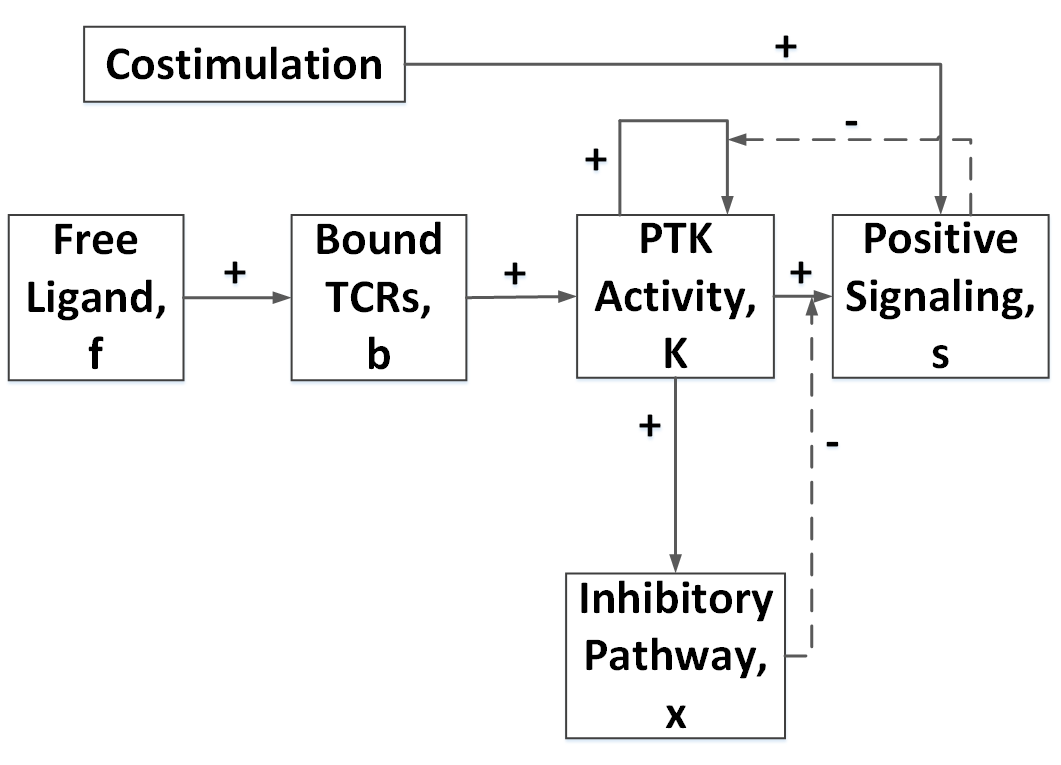
\includegraphics[scale=0.275]{figures/Fig6.png}}
	}}
      
      \caption{Network graph of the T-cell receptor kinetics model, where rectangles denote input nodes, the other nodes denote state nodes, particularly the nodes with shadows are chosen to be observed.}
      \label{fig:6}
  \end{figure}

As the wide application of \BCNs, it is important to research the control-theoretic problems of \BCNs. The study on control-theoretic problems of \BCNs\ can date back to 2007 \cite{Akutsu2007Control}. The work above also proves that the problem of determining the controllability of \BCNs\ is {\em NP}-hard in the number of nodes. Furthermore, it points out that ``One of the major goals of systems biology is to develop a control theory for complex biological systems.'' Since then, the study on control-theoretic problems in the areas of \BNs\ and \BCNs\ has drawn great attention \cite{cheng2009controllability, Zhao2010Input, Cheng2011Identification, Cheng2011Analysis,Fornasini2013Observability}. Besides controllability, observability is an another  basic control-theoretic problems and it also attract many attentions.  Among these studies, \emph{semi-tensor product} (STP) of matrices is one of useful tool to deal with  both \BNs\ and \BCNs\  related problems \cite{cheng2009controllability}.  Moreover,  \cite{cheng2009controllability} gives equivalent conditions for controllability of \BCNs\ and observability of controllable \BCNs. To date, there are four types of observability have been proposed. 

\begin{enumerate}
	\item The first type of observability proposed in 2009 \cite{cheng2009controllability} means that every initial state can be determined by an input sequence.
	
	\item 
	The second observability proposed in 2010 \cite{Zhao2010Input} stands that for every two distinct initial states, there exists an input sequence which can distinguish them, and this observability is determined in \cite{Li2015Controllability}.
	
	\item The third observability proposed in 2011 \cite{Cheng2011Identification} states that there is an input sequence that determines the initial state.
	
	\item  The fourth observability proposed in 2013 \cite{Fornasini2013Observability} is essentially the observability of linear control systems, i.e., every sufficient long input sequence can determine the initial state.
\end{enumerate}
 

%\tl{can you state the four types observability clearly and formally here?}

%\rev{****input s equence***}

In above mentioned definitions an input is not the value of an input-node, but it represents the values of all input-nodes of the \BCN\ on a time step. Therefore, an input can be seen as a vector of the values of all input-nodes of the \BCN\ on a time step. An input sequence consists of several inputs in sequential time steps.
     A output can also be seen as a vector of the values of all output-nodes of the \BCN\ on a time step. In every time step, there is a pair of input and output of \BCN. A output sequence also consists of several outputs in sequential time steps. In the following, we will list the informal definition of four offline  observabilities as well as the formal definition of four observabilities.% in the following pages.
 
The four  types of observability  have many nice properties that they can be used in some useful applications. However, all of four  types of observability of \BCNs\ are offline observabilities which means that they can not adjust the input sequence by observing the output sequence in the process of determining the initial state of \BCNs. Therefore, we propose the online observability that we can determine the initial state of \BCNs\ dynamically. In other words,  the online observability decides the input sequence in each time step by observing the out sequence. In the  online observability, we infer the possible  initial states set by observe the  first $k$ time steps output of \BCN. Through the  possible  initial states, we can choose one of input to refine the possible initial states set in the time step $k+1$. Repeat above procedure until the cardinality of initial states set turns into be one. We call this process is a dynamic process. 

\subsubsection*{Contribution}
Firstly, we propose the concept of the online observability of \BCNs. Compared with four existing observabilities, the online observability can help us to determine the initial state of some biological systems which can be checked at most once. Secondly, in addition to theoretical research, we also provide two algorithms to determine the online observability for \BCNs. Finally, we introduce some applications of the online observability of \BCNs. Including takes less observation costs, methods to find shortest path and approaches to avoid entering critical states when we use it to determine the initial state of \BCNs.  These applications will explain the advantages of online observability of \BCNs\ comparing with offline observabilities. %\rev{No important points}%\rev{***Compare with offline observabilities****} 
\subsubsection*{Structure}
The remainder of this paper is organized as follows. {\em Section \ref{sec:pre}} introduces necessary preliminaries about \BCNs, algebraic forms of \BCNs\ and the four existing kinds of observability of  \BCNs. {\em Section \ref{sec:online}} presents the definition of deduction function, $k$ steps determinability and online observability of \BCNs. {\em Section \ref{sec:deter}} presents how to determine the online observability of \BCNs\ by super tree and directed graph. {\em Section \ref{sec:app}} talks about some applications of the online observability of \BCNs. We also compare the online observability with offline observabilities in this section. {\em Section \ref{sec:con}} ends up  with the introduction of some future works.

%\tl{I will try to rewrite the intro.}

%==============================================================================================================
% !Mode\dots ``TeX:UTF-8''
% !TEX root = ../root.tex
\section{Preliminaries} 
\label{sec:pre}
In this section we introduce the definition of \BCNs\ and their algebraic form as well as the four existing kinds of observability of {\em BCNs}.



\subsection{Boolean Control Networks}

A Boolean control network can be described as a directed graph together with logical equations to describe the updating rules of the nodes of this directed graph, the definition of \BCN\ is as follows. 

\begin{definition}
(\cite{Ideker2001A}) A \BCN\ consists of input-nodes, state-nodes, output-nodes, and directed edges which connect nodes. A node in \BCN\ can take a logic value from $\{0,1\}$ at a discrete time $0, 1, 2,\ldots$ For one directed edge from a state-node $s_1$ (or an input-node $i_1$) to a state-node $s_2$ means that the logic value of $s_2$ at time step $t+1$ is affected by the value of $s_1$ (or $i_1$)  at time step $t$. For one directed edge from a state-node $s_1$ to a output-node $o_1$ means that the logic value of $o_1$ at time step $t$ is affected by the value of $s_1$  at time step $t$. 
\end{definition}


Note that one can only know that whether a node is affected by another node from the network graph. Different \BCNs\ may have the same structure, in order to determine a \BCN\ uniquely, logical equations are also needed to describe the specific updating rules of \BCNs.

 
 \begin{figure}[thpb]
      \centering
      \framebox{\parbox{3in}{
		\centerline{\includegraphics[scale=0.23]{figures/Fig1.png}}
	}}
      
      \caption{A Boolean control network with two input-nodes $A$ and $B$, four state-nodes $C$, $D$, $E$ and $F$, and two output-nodes $G$, $W$. We use blue, black and orange, to distinguish three kinds of nodes and three kinds of edges.}
      \label{fig:1}
  \end{figure}

To better illustrate the concept of {\em BCNs}, we give a simple example to describe it.

\begin{example}
	In Fig.\ref{fig:1} we have a \BCN\ with two input-nodes $A$ and $B$, four state-nodes $C$, $D$, $E$ and $F$, and two output-nodes $G$, $W$. The \BCN\ is shown in Fig.\ref{fig:1}, and the updating rules of this \BCN\ are described as truth table Fig.\ref{fig:2}. The reason why we use truth table to describe the updating rules of the \BCN\ is that this form of updating rules will be more convenient for \BCN\ to be converted into its aglebraic form. What's more, for instance, the updating rule of state-node $G$ is that,
	\[G(t)=C(t)\wedge \neg(\neg{D(t)}\wedge \neg E(t)\wedge \neg F(t))\]
	
	For convenience, we will use this example in the whole paper to explain various concepts we introduce.
  \begin{figure}[thpb]
      \centering
      \framebox{\parbox{3in}{
		\centerline{\includegraphics[scale=0.26]{figures/Fig2.png}}
	}}
      
      \caption{The truth table which describe the updating rules of the \BCN\ shown in {\em Fig.\ref{fig:1}}.}
      \label{fig:2}
   \end{figure}
\end{example}   


%==============================================================================================================
\subsection{The algebraic forms of \BCNs}
To better illustrate the concept of algebraic forms, in this paper, we investigate the \BCN\ in the following. And we suppose that this \BCN\ has $n$ state-nodes, $m$ input-nodes and $q$ output-nodes. Then the updating rules of the \BCN\ can be described as following formulas:
\begin{equation}
\begin{split}
s(t+1)=&f(i(t),s(t))\\
o(t)=&h(s(t))
\end{split}
\label{equ:1}
\end{equation}
$s(t)\in \mathbb{B}^n$ are state-nodes; $i(t)\in \mathbb{B}^m$ are input-nodes; $o(t)\in \mathbb{B}^q$ are output-nodes; $f:\mathbb{B}^{n+m}\mapsto \mathbb{B}^n$ and $h:\mathbb{B}^n\mapsto \mathbb{B}^q$ are logical functions that represent the updating rules of {\em BCNs}. Where $\mathbb{B}$ : the set $\{0,1\}$; $t=0,1,\ldots$ represents the discrete time. 

Therefore in the previously mentioned example, we have that $C(t), D(t), E(t), F(t)\in s(t)$; $A(t), B(t)\in i(t)$ and $G(t), W(t)\in o(t)$; $n=4$, $m=2$ and $q=2$; $f$ and $h$ are described in the truth table ({\em Fig.\ref{fig:2}}). 

Furthermore, the {\em STP} of matrices can be used to represent the algebraic forms of \BCNs\ \cite{cheng2009controllability}, the definition of {\em STP} is as follows.

\begin{definition}[STP] 
	\cite{Cheng2011Analysis} Let $X\in\mathbb{R}_{m\times n}$, $Y\in\mathbb{R}_{p\times q}$ and $\alpha=lcm(n,p)$ be the least common multiple of $n$ and $p$. The STP of $X$ and $Y$ is defined as \[X\ltimes Y=(X\otimes I_{\alpha/n})(Y\otimes I_{\alpha/p}),\] where $\otimes$ denotes the Kronecker product. 
\end{definition}

After introducing the definition of {\em STP} of matrices,  we introduce some related notations at first \cite{Zhang2016Observability}:
\begin{itemize}
  \item $\delta^i_n$: the $i$-th column of the identity matrix $I_n$;
  \item $\Delta_n$: the set $\{\delta^1_n,\ldots,\delta^n_n \}$; 
  \item $\delta_n \left[i_1,\ldots,i_s\right]$: $\left[\delta^{i_1}_n,\ldots,\delta^{i_s}_n\right]\left(i_1,\ldots,i_s\in\left\{1,2,\ldots,n\right\}\right)$ the logical matrix;
  \item  $L_{n\times s}$: the set of $n\times s$ logical matrices.
\end{itemize}


Using {\em STP} of matrices, the formula (\ref{equ:1}) can be quivalently represented in the following algebraic form:
\begin{equation}
\begin{split}
s(t+1)=&L\ltimes{i(t)}\ltimes{s(t)}\\
o(t)=&H\ltimes{s(t)}
\end{split}
\label{equ:2}
\end{equation}
where $s(t)\in\Delta_N$, $i(t)\in\Delta_M$, and  $o(t)\in\Delta_Q$ denote the states, inputs and outputs respectively the same as in formula {\em (\ref{equ:1})}, but $s(t)$, $i(t)$ and $o(t)$ in formula {\em (\ref{equ:2})} would be written in special vector forms; $L\in L_{N\times\left(NM\right)}$ and $H\in L_{Q\times N}$ denote the relation matrices; that $N=2^n$, $M=2^m$, and $Q=2^q$. Since {\em STP} keeps most properties of the conventional product \cite{Cheng2011Analysis}, the associative law, the distributive law, etc., we usually omit the symbol ``$\ltimes$'' hereinafter. For instance, the 
formula ``$s(t+1)=L\ltimes{i(t)}\ltimes{s(t)}$'' will be written as ``$s(t+1)=L{i(t)}{s(t)}$'' in the following pages.

To construct algebraic form (\ref{equ:2}) we give a mapping $\tau:\{0,1\}\mapsto \{\delta_2^1, \delta_2^2\}$ where $\tau(0)=\delta_2^2$, $\tau(1)= \delta_2^1$. 
%each logical value a vector form as: $1 \scriptsize{\sim} \delta_2^1$, $0 \scriptsize{\sim} \delta_2^2$. 
Therefore, the logical variable $A(t)$ takes value from these two vectors, i.e., $A(t)\in \{\delta_2^1, \delta_2^2\}$. Using the {\em STP} of matrices, we have 
\[i(t)=i_1(t){\ldots}i_m(t);\] 
\[s(t)=s_1(t){\ldots}s_n(t);\] 
\[o(t)=o_1(t){\ldots}o_q(t).\] 
And according to \cite{Cheng2003Semi}, each logical function $f_p$ of state-nodes can be found in the updating rules (\ref{equ:1}). The form of  $f_p$ as:
\[f_p(i_1(t),\ldots,i_m(t),s_1(t),\ldots,s_n(t))\] 
and there exists a structure matrix $L_p\in L_{2\times {NM}}$ such that
\begin{equation}
\begin{split}
\tau(f_p(i_1(t),\ldots,i_m(t),s_1(t),\ldots,s_n(t)))= L_pi(t)s(t)
\end{split}
\end{equation}
%where the left side of equation calculate the truth value and the  right side of equation calculate the vector in $\{\delta_2^1, \delta_2^2\}$. 
For state-nodes $s_1,\ldots,s_n$, we have $n$ logical matrices $L_1,\ldots,L_n$ for them, respectively. 
%We have that
%when\\
If for each state-node $s_p$ the logical matrix has its form
\[L_p=[\delta_2^{p_1},\ldots,\delta_2^{p_{NM}}],\] 
then we have that %for the set of all state-nodes $s(t)$ the logical matrix 
\[L=[\delta_N^{R_1},\ldots,\delta_N^{R_{NM}}]\]  where 
\[\delta_N^{R_1}=\delta_2^{1_1}\ldots\delta_2^{n_1};\ldots; \delta_N^{R_{NM}}=\delta_2^{1_{NM}}\ldots\delta_2^{n_{NM}}.\] 
%then 
By this relationship we can construct the $L$ for the algebraic forms of \BCNs. What's more we can also construct the logical matrix $H$ in the similar way. To better illustrate the concept of algebraic forms, we give a simple example to describe it.
\begin{example}
For instance, the \BCN\ whose structure is depicted in Fig.\ref{fig:1}, and the updating rules of this \BCN\ is described as truth table in Fig.\ref{fig:2}. We have that the updating rules of this \BCN\ can be represented with the algebraic form:
\begin{equation}
\begin{split}
s(t+1) =&\delta_{16}[\alpha]i(t)s(t)\\
o(t) =&\delta_4[\beta]s(t)\\
\end{split}
\label{equ:4}
\end{equation}
where $\alpha=\{10,4,11,16,9,5,1, 7,15,2,3,12,7,6,8,13,8,9,\\15,10,14,4,3,16,1,14,12,13,5,7,2,6,7,2,3,13,13,9,5,1,\\16,13 ,6,14,11,10,4,15,1,14 ,7,6,9 ,8,11,12,5,5,13,3,10,\\12,16,16\}$, $\beta=\{1,1,1,2,2,2,2,3,3,3,3,4,4,4,4,4\}$, $t\in \mathbb{N}$, $s\in \Delta_{16}$, $i\in \Delta_4$ and $o\in \Delta_4$.
\end{example}   
\subsection{Four existing observability of \BCNs}
In this subsection we introduce four existing kinds of observability of \BCNs. Let $\Delta_N$, $\Delta_M$, $\Delta_Q$ be three alphabets, for all $s_0\in \Delta_N$ and all $p\in \mathbb{Z}_+$; $\infty$ is the infinite natural numbers. In order to introduce four existing kinds of observability of {\em BCNs}, we define the mappings \cite{Zhang2016Observability}:
\begin{equation}
\begin{split}
L^p_{s_0} &: (\Delta_M)^p\mapsto(\Delta_N)^p, i_0\ldots i_{p-1} \mapsto s_1 \ldots\, s_p\\
L^{\infty}_{s_0} &: (\Delta_M)^{\infty}\mapsto(\Delta_N)^{\infty}, i_0 i_1 \ldots  \mapsto s_1 s_2 \ldots
\end{split}
\end{equation}
\begin{equation}
\begin{split}
(HL)^p_{s_0} &: (\Delta_M)^p\mapsto(\Delta_Q)^p, i_0\ldots i_{p-1} \mapsto o_1\ldots\, o_p\\
(HL)^{\infty}_{s_0} &: (\Delta_M)^{\infty}\mapsto(\Delta_Q)^{\infty}, i_0 i_1 \ldots  \mapsto o_1 o_2\ldots
\end{split}
\end{equation}

For all  $p\in \mathbb{Z}_+$, all $I=i_1 \ldots i_p \in(\Delta_M)^p$, and all $1\ge p \ge j \ge |I|$, we use I[p,j] to denote the word $i_p \ldots i_j$ as a input sequence. Then four existing kinds of observability of BCNs can be define as: 
\begin{definition}
The first kind of observability is that, \BCN\ is called observable, if for every initial state $s_0 \in \Delta_N$, there exists an input sequence $I\in(\Delta_M)^p$ for some $p\in \mathbb{Z}_+$ such that for all states $s_0\neq {s'}_0\in \Delta_N$, $Hs_0=H{s'}_0$ implies $(HL)^p_{s_0}(I)\neq (HL)^p_{{s'}_0}(I)$ \cite{cheng2009controllability}.
\end{definition}

Hence the first observability means that if a \BCN\ is observable then every initial state of the \BCN\ can be determined by an input sequence. But we can only use the corresponding input sequence of a state to check whether this state is the initial state of the {\em BCN} or not.
\begin{definition}
	The second kind of observability is that a \BCN\ is called observable if for any distinct states $s_0$, ${s'}_0 \in \Delta_N$, there exists an input sequence $I\in(\Delta_M)^p$ for some $p\in \mathbb{Z}_+$, such that $Hs_0=H{s'}_0$ implies $(HL)^p_{s_0}(I)\neq (HL)^p_{{s'}_0}(I)$ \cite{Zhao2010Input}.
\end{definition}

The second observability means that a \BCN\ is called observable if for every two distinct initial states of the {\em BCN}, there exists an input sequence which can distinguish them. 
\begin{definition}
	The third kind of observability is that, a \BCN\ is called observable, if there exists an input sequence $I\in(\Delta_M)^p$ for some $p\in \mathbb{Z}_+$, such that for any distinct states $s_0$, ${s'}_0 \in \Delta_N$, $Hs_0=H{s'}_0$ implies $(HL)^p_{s_0}(I)\neq (HL)^p_{{s'}_0}(I)$ \cite{Cheng2011Identification}.
\end{definition}

The third observability means that a \BCN\ is called observable if there is an input sequence that determines the initial state of the {\em BCN}.
\begin{definition}
	The fourth kind of observability is that, \BCN\ is called observable, if for any distinct states $s_0$, ${s'}_0 \in \Delta_N$, for any input sequence $I\in(\Delta_M)^{\infty}$, $Hs_0=H{s'}_0$ implies $(HL)^{\infty}_{s_0}(I)\neq (HL)^{\infty}_{{s'}_0}(I)$ \cite{Fornasini2013Observability}.
\end{definition}

The fourth observability means that a \BCN\ is called observable if every sufficient long input sequence can determine the initial state of the \BCN.

Then from the definitions of  four existing kinds of observability, we know that \cite{Zhang2016Observability}:
\begin{itemize}
  \item the first one implies the second one;
  \item the third one implies the second one and first one;
  \item the fourth one implies the third one, second one and first one.
\end{itemize} 
%, when we don't presuppose the initial state of {\em BCNs}
 
We can not use the first one and second one to determine the initial state of \BCNs\ which can be checked at most once. For example, in the first kind observability we need to assume the initial state of a \BCN, and then check it by corresponding input sequence of this state. If the state we assume is correct, then we can determine the initial state. But if the the assumption is not correct, we can not determine the initial state of the \BCN. Therefore we need to check several test cases (with the same initial state) of this \BCN\ untill we can determine the initial state of it. However we can use the third existing observability and fourth existing observability to determine the initial state of \BCNs\ through one test case. And we need not to presuppose the initial state of \BCNs\ when we use the third observability and fourth observability. But the requirements for \BCNs\ are very harsh when we use the third observability and fourth observability.
 
In some biological systems, the initial states of them can be checked at most once, i.e., we have only one test case for them. Therefore, we can not use the first observability and second observability to determine the initial states of them in real time. And in some biological systems, it would takes many costs to check these biological systems. Hence we will spend a lot of overhead to determine the initial states of them by the first observability and second observability. Furthermore, we also can not use the third observability and fourth observability to determine the initial states of some biological systems when they can not satify the requirements of the third observability and fourth observability. With these disadvantages of four existing observabilities, we propose the online observability of \BCNs\ to solve this problem.
 \subsubsection*{Problem}
Finding the necessary and sufficient condition of determine the initial state of \BCNs\ in real time.
% !Mode\dots ``TeX:UTF-8''
% !TEX root = ../root.tex
\section{The online observability of \BCNs}
\label{sec:online}
In this paper we propose the online observability, the informal definition of it is as follows. 

\begin{definition}
	A \BCN\ is called online observable, if every initial state $s_0 \in \Delta_N$ can be determined in one time by dynamically deciding input sequence and observing output sequence at every step without presupposing the  initial state of \BCN. And this process can be accomplished in finite steps.
\end{definition}

%\tl{maybe I did not understand this, but I think you are confusing two things: the observability and the algorithm (approach) to determine the initial state. It seems to me that you are describing a new approach (the online approach), but does this change the observability? if yes, how? Is this a stronger notion or a weaker notion or incomparable?}

In this section, firstly we present the definition of deduce function, secondly we present the definition of $K$ steps deterministic. We take them as the preparations for defining online observability. Finally, we give the formal definition of online observability of \BCNs. 
\subsection{Deduce function}
Different from four existing types, the observability we propose can determine the initial state online. Because in the process of determining the initial state every input of the input sequence is decided by the output we observe at every time step. At the beginning, we can observe the output of \BCNs, so that we can infer the possible values of state-nodes and treat them as possible states set $S_0$. Then as we can know the possible states set, we need to decide the input $i_0$. The input $i_0$ will make sure any different possible states $s_i, s_j \in S_0$ will not turn into the same state after affected by input $Ls_i i_0\neq Ls_j i_0$. After decided input, we can observe the new output, and then we can infer the new possible states set. The cardinal number of possible states set after we inputted will not lager than the cardinal number of possible states set before we input. If the cardinal number of possible states set turn into be $1$ then we can determine the state and the initial state of {\em BCN}. To simulate this deduction process, we give the definition of deduce function that.
\begin{definition}[Deduce Function] The deduce function can be defined as $D\left(S, I, O\right)$. Based on deduction process, we have for any \[s_i(t+1)\in D\left(S, I, O\right)\] there exists the corresponding $s_i(t)\in S$ of $s_i(t+1)$ that \[s_i(t+1)=LIs_i(t)\] and \[O=Hs_i(t+1).\]
\end{definition}
where   
\begin{itemize}
  \item $S\in 2^{\Delta_N}$ is the possible states set;
  \item $I\in\Delta_M$ represents the input;
  \item $O\in\Delta_Q$ represents the output; 
  \item $D\left(S, I, O\right)\in 2^{\Delta_N}$ is the possible states set after deduction.
\end{itemize} 
 
 From the definition of deduce, we have some equations for this function that
\begin{equation}
\begin{split}
D\left(\varnothing,I_i,O_i\right)=\varnothing\\
%D\left(\varnothing,I_i,O_i\right)=D\left(\varnothing,\varepsilon,O_i\right)= &D\left(\varnothing,\varepsilon,\varepsilon\right)=\varnothing\\
\end{split}
\label{equ:7}
\end{equation}

Equation (\ref{equ:7}) represents that if the possible states set is an empty set $\varnothing$, no matter what we do we can only deduce the possible set is $\varnothing$. 
\begin{equation}
\begin{split}
D\left(S_i,\varepsilon,\varepsilon\right)=&S_i\\
\end{split}
\label{equ:8}
\end{equation}

If the possible states set is $S_i$ and we neither input anything and nor observe the output. In this case we can only deduce that the possible states set is $S_i$ shown in equation (\ref{equ:8}).
\begin{equation}
\begin{split}
D\left(\Delta_N,\varepsilon,\delta_4^1\right)=&\{\delta_{16}^1,\delta_{16}^2,\delta_{16}^3\}\\
\end{split}
\label{equ:9}
\end{equation}
 
 Using the example mentioned before, when the possible states set $S_i=\Delta_N$, and  we observe that the outputs of \BCN\ is $\delta_4^1$ before we decide input. In this case we can deduce that the possible states would be $\delta_{16}^1$, $\delta_{16}^2$ or  $\delta_{16}^3$ shown in equation (\ref{equ:9}).
\begin{equation}
\begin{split}
D\left(\{\delta_{16}^1,\delta_{16}^2,\delta_{16}^3\},\delta_4^1,\varepsilon\right)=&\{\delta_{16}^{10},\delta_{16}^4,\delta_{16}^{11}\}\\
\end{split}
\label{equ:10}
\end{equation}

If the possible states set $S_i=\{\delta_{16}^1$, $\delta_{16}^2$, $\delta_{16}^3\}$ we input $\delta_4^1$. Before we observe the output of \BCN\ we can only deduce the possible states would be   $\delta_{16}^{10}$, $\delta_{16}^4$ or  $\delta_{16}^{11}$ shown in equation (\ref{equ:10}).
\begin{equation}
\begin{split}
D\left(\{\delta_{16}^1,\delta_{16}^2,\delta_{16}^3\},\delta_4^1,\delta_4^3\right)=&\{\delta_{16}^{10},\delta_{16}^{11}\}\\
\end{split}
\label{equ:11}
\end{equation}

But if we observe that the output of \BCN\ is $\delta_4^3$, then we can deduce that the possible state can be $\delta_{16}^{10}$ or  $\delta_{16}^{11}$ shown in equation (\ref{equ:11}); 
\begin{equation}
\begin{split}
D\left(\{\delta_{16}^4,\delta_{16}^5,\delta_{16}^6\},\delta_4^3,\varepsilon\right)=&\{\delta_{16}^9,\delta_{16}^{13}\}
\end{split}
\label{equ:12}
\end{equation}

 Finally if the set of states is $\{\delta_{16}^4,\delta_{16}^5,\delta_{16}^6\}$ and the inputs is $\delta_4^3$. Before we observe the output of \BCN\ we can deduce that the possible state values can be $\delta_{16}^9$ or  $\delta_{16}^{13}$ shown in equation (\ref{equ:12}), as  the cardinality number of the possible states set decreased, we can't deduce the initial state any more. 

\subsection{$K$ steps deterministic}
After we difined the deduce function, we can present the definition of $K$ steps deterministic of the states set of \BCNs\ and the range of $K$ is the set of natural numbers. It may easier to difine online observability by programming language. But we would like to define its mathematical form for preciseness of concepts. Therefore, before defining the online observability of \BCNs, we need to difine the $K$ steps deterministic of the states set of \BCNs at first.
\begin{definition}[$K$ Steps Deterministic] 
When $K=0$, 
 if for a set of states $S'$ and $|S'|=1$, then $S'$ is $K$ step deterministic. When $K>0$, 
 if for a set of states $S'$ ($|S'|>1$), there exists $I'$ in $\Delta_M$ implies \[|D\left(S',I',\varepsilon\right)|=|S'|, \]and implies ``For every $O'$ in $\Delta_Q$, \[|D\left(S',I',O'\right)|\neq 0\] implies $D\left(S',I',O'\right)$ is {\em$K'$ (${K'}<K$)} stepes deterministic.', then $S'$ is $K$ steps deterministic.
\end{definition}

From the definition of {\em$K$} steps deterministic we know $K=0$ means that we can determine the state without any input and observing output. Because if we know the cardinality number of possible states set is $1$, then we can know the state of \BCNs. We can only discuss the case of $K=0$ when $|S'|=1$. If $K>0$, then the definition of $K$ steps deterministic is defined recursively, and it need to use the definition of $K$ ($K=0$) steps. When we talk that a states set of \BCNs\ is $k$ steps deterministic we default $k\ge0$.

Furthermore, if $S'$ is $k_1$ steps deterministic and $k_1\leq k_2$, then $S'$ is $k_2$ steps deterministic. But if $S'$ is $k_1$ steps deterministic and $k_1\geq k_2$, we can not make sure whether $S'$ is $k_2$ steps deterministic or not. Therefore you can consider the ``$S'$ is $k_i$ steps deterministic'' as ``We can determine the state of a \BCN\ with possible states set $S'$ in $k_i$ steps. And we finish this process by deciding input sequence and observing out sequence at each time step''. 
\subsection{Online Observability}
After the previous preparation, we present the formal definition of the online observability. The formal definition of the online observability of {\em BCNs} is as follows.
\begin{definition}[Online Observability of  BCNs]
If for every  $O'$ in $\Delta_Q$ and $|D\left(\Delta_N,\varepsilon, O'\right)|\neq 0$, there exists a $ k \ge 0$ implies $D\left(\Delta_N,\varepsilon,O'\right)$ is $k$ stepes deterministic, then this \BCN\ is online observable. We even can define it simpler, if there exists $k \ge 0$ implies $\Delta_N$ is $k$ stepes deterministic, then this \BCN\ is online observable. 
\end{definition}

The difference between the second definition and the first definition is that whether we observe the corresponding output of the initial state of \BCN\ at first. For better performance, we use the first definition of online observability.

After defining online observability of \BCNs, we discuss the comparison of online observability with the four existing observability. In the second existing kind of observability, we presuppose the initial state of \BCNs, and then try to find the input sequence to distinguish it from other kinds of initial states. But the input sequence determined by the presupposed initial state may make other kinds of initial states turn into be the same state, so that other kinds of initial states can't be determined anymore. This problem has to be considered in the online obervability of \BCNs. Hence the online observability implies the first existing kind of observability, and then the online observability implies the second existing kind of observability. In the third existing kind of observability, there has to exist an input sequence that can distinguish any distinct states. However in online observability we can use different input sequences to distinguish any distinct states in different states sets. These different states sets are classified by their corresponding output. Therefore, we have the third existing kind of observability implies the online observability of \BCNs, then the fourth existing kind of observability implies the online observability.

When I learn the existing four kinds of observability of \BCNs, I find that if we want determine the initial state of a \BCNs\ by first kind of observability, we need to guess the initial state of the \BCN\ and then check it by its corresponding input sequence, if the initial state we guess is right, we can determine it, but if not, we need to guess again and input the corresponding input sequence untill we determine the initial state of the \BCN. But if we can't repeat this process, we may can't determine the initial state of the \BCN\ any more. Then I turn my gaze to the third observability, this kind of observability makes we can determine the initial state without presupposing the initial state. But I think if we can determine the possible states set of the \BCN\ by observing the output at first, why can't we try to find corresponding input sequence for them? And then my teacher and I talk about this thinkness and expand it into the original idea of the online observability of \BCNs. 

From the informal definition and formal definition of online observability, we can know that the necessary and sufficient condition of determine the initial state of \BCNs\ without presuppose the initial state is the online observability of \BCNs. By this definition we can build \BCNs\ with least output-nodes when we want to determine the initial state of \BCNs.
%==============================================================================================================
% !Mode\dots ``TeX:UTF-8''
% !TEX root = ../root.tex
\section{Determining the online observability of \BCNs}
\label{sec:deter}
In this paper, we propose two approaches to determine the online observability of \BCNs. The first way is by using supertree and the second way is by using directed graph. The construction process of supertree and directed graph simulate deduction process mentioned before. We check the super tree based on the definition of online observability of \BCNs\ depth first or breadth first. When we find enough leaf nodes, we can make sure the \BCN\ is online observable. But when we used the super tree to determine the online observability of \BCNs, we need to check the existence of loops when we build the super tree. And many nodes in the tree are repeated, these nodes will take a lot of time overhead and space overhead when we check the super tree. Therefore, we proposed the second way to determine the online observability of \BCNs\ by using directed graph. By this way we can avoid checking the existence of loop and avoid checking repeated nodes. There are also other advantages which help us select the input smarter when we use the second way. All of these advantages will reduce time and space overhead to determine the initial state of a \BCN. If a \BCN\ seems to be online observable we would check it earlier by using supertree. But if a  \BCN\ not seems to be online observable we prefer to check it earlier by using directed graph. If we just want to find a path to determine the initial state of a \BCN\ we would check it by using supertree. But if we want find all paths to determine the initial state of a \BCN\ and make some optimizations in the process of determine the initial state we prefer to check it by using directed graph.

\subsection{Algorithm implemented by supertree} As we mentioned before, we can use the deduction function to determine the initial state of \BCNs. According to the definition of online observability we will alternately observe the output and decide the input. When the  cardinal number of the states set comes into be $1$ we can determine the initial state, and stop deducing the initial state of \BCNs. According to this process, we can define the supertree for \BCNs. For convenience, we use the states set inside the node to represent the node, and output in the edge to represent the edge.
\begin{definition}[Super Tree]
The root node of the super tree is $\Delta_N$, the leaf nodes of the super tree are the nodes with cardinal number $1$ ($|S_i|=1$). In addition to the leaf nodes, if a node $S_i$ in the $2k + 1$ ($k\in \mathbb{N}$) layer of the supertree and 
\[|\Ded\left(S_i,\varepsilon, o_j\right)|>0,\]
 then $\Ded\left(S_i,\varepsilon, o_j\right)$ is one of its son nodes, and $o_j$ is the edge from $S_i$ to $\Ded\left(S_i,\varepsilon, o_j\right)$. If a node $S_i$ in the $2k+2$ layer of the supertree and  
\[|\Ded\left(S_i,i_p,\varepsilon\right)|=|S_i|,\] 
then $\Ded\left(S_i,i_p,\varepsilon\right)$ is the son node of $S_i$ and $i_p$ is the edge from $S_i$ to $\Ded\left(S_i,i_p,\varepsilon\right)$. 
\end{definition}

  \begin{figure}[thpb]
      \centering
      \framebox{\parbox{3in}{
		\centerline{\includegraphics[scale=0.067]{figures/Fig3.png}}
	}}
      
      \caption{Branch of the super tree which represents $\{\delta_{16}^1,\delta_{16}^2,\delta_{16}^3\}$. The blue edges and orange edges show the observing output processes and deciding input processes, respectively. The yellow nodes are leaf nodes.}
      \label{fig:3}
   \end{figure}

At the beginning we infer that the possible states set is $\Delta_N$, thus the root node of the super tree is $\Delta_N$. When the cardinal number of the possible states set turns into $1$, we can determine the state of \BCN. Therefore, the leaf nodes of the super tree are the nodes with cadinal number $1$. We observe the output of \BCN\ to infer the possible states set of \BCN\ at first. After that, we decide the input and infer the new possible states set. We alternately observe the output and decide the input untill we can determine the state of {\em BCN}. Therefore we use $\Ded\left(S_i,\varepsilon, o_j\right)$ to find son nodes for every $S_i$ in $2k+1$ layer, and using $\Ded\left(S_i,i_p,\varepsilon\right)$ to find son nodes for every $S_i$ in $2k+2$ layer. The formula $|\Ded\left(S_i,\varepsilon, o_j\right)|>0$ ensures the node $\Ded\left(S_i,\varepsilon, o_j\right)$ has meaning. The formula $|\Ded\left(S_i,i_p,\varepsilon\right)|=|S_i|$ guarantee we can determine the state of \BCN\ in the end. 
\begin{example}
For example, the \BCN\ whose structure is depicted in Fig.\ref{fig:1}, and the updating rules of this \BCN\ is described as truth table in Fig.\ref{fig:2}. The Fig.\ref{fig:3} show branch of the tree which represents $\{\delta_{16}^1,\delta_{16}^2,\delta_{16}^3\}$ and its deduction process. The nodes represent the states sets, the blue edges represent the observing output processes, and the orange edges represent the deciding input processes. This branch is not completed, because only the yellow nodes are the leaf nodes. If we want to find all of the ways to determine the initial state of \BCN, we have to build the complete tree for \BCN. This process takes many additional time and space overhead. Especially when there are loops in the tree, like the $\{\delta_{16}^2,\delta_{16}^3\}$ in fourth layer and the $\{\delta_{16}^2,\delta_{16}^3\}$ in fifth layer that will form a loop. In this case we can never build the complete tree, thus we need to check the existence of loops and omit it. There are also some nodes take the same states set which will also take additional overhead. For instance there are two nodes take the same states set $\{\delta_{16}^1,\delta_{16}^{16}\}$ in the fifth layer. However, it would be a lot easier if we only need to find a way to determine the initial state. For instance, when we find the leaf nodes $\delta_{16}^1$, $\delta_{16}^7$ and  $\delta_{16}^{14}$ in third layer by breadth-first algorithm, we can make sure that the states set $\{\delta_{16}^1,\delta_{16}^2,\delta_{16}^3\}$ is 1 step deterministic. After that, we use this conclusion to determine the initial state of \BCN. 
\end{example}   
\subsection{Algorithm implemented by directed graph}
To improve the shortcomings of the way by using supertree, we proposed the way by derected graph wich may takes less time and space overhead. The most difference between supertree and derected graph is that supertree is built from the root node to leaf nodes. However, the derected graph is built from smaller nodes (contain fewer states) to larger nodes (contain more states). There is not any repeated node in the derected graph because any node only appears once in the graph. And even there are some loops in the derected graph, the loops would not influence us to build the directed graph completely.

The construction algorithm of derected graph is shown in the Algorithm.\ref{alg:1}. The algorithm to build nodes used in the Algorithm.\ref{alg:1} is shown in the Algorithm.\ref{alg:2}.

\begin{algorithm}[h]
\caption{Algorithm to construct the directed graph of \BCNs}
\begin{algorithmic}[1]
\REQUIRE 
The algebraic forms of \BCN
\ENSURE  
The directed graph of \BCN
\STATE  $k=1$ (The number of states in the nodes)\
\STATE  $Ob=$ false (The online observability of \BCN)\
\STATE  $N_i$ (Node)\
\STATE  $i_p$ (Input)\
\STATE  $NodesArray$ (Nodes array)\
\STATE  $Sis$ (The suitable inputs set of $N_i$)\
\STATE {\sf buildnode}(k)
\STATE $k= k+1$
\WHILE {NodesArray={\sf buildnode}(k)!=Null}
\STATE NodesArray={\sf buildnode}(k)
\FOR{each $N_i\in NodesArray$}
\IF{$k==2$}
\STATE $Sis$ = $\Delta_M$ 
\ELSE

\STATE Find $Sis$ by other nodes

\ENDIF
\FOR{each $i_p \in Sis$}
\STATE Check $N_i$ by $i_p$
\STATE Build edges for $N_i$ 
\ENDFOR
\IF {$N_i$ has not any edge.}
\STATE $Ob=0$ 
\STATE return Null
\ENDIF
\ENDFOR

\STATE $k= k+1$
\ENDWHILE
\STATE $Ob=1$ 
%\STATE return $Ob$
\STATE return $NodesArray$
\end{algorithmic}
 \label{alg:1}
\end{algorithm}
 The algorithm to build nodes used in the Algorithm.\ref{alg:1} is shown in the Algorithm.\ref{alg:2}.
\begin{algorithm}[h!]
\caption{{\sf buildnode}(int k)}
\begin{algorithmic}[1]
\REQUIRE 
The number of states in the nodes $k$
\ENSURE  
The nodes with $k$ states whose corresponding outputs are the same%, and the outputs of $p$ states inside one node are the same.
%\STATE {\sf buildnode}(int p)
%\STATE  \{ 
%\dfSTATE $p=p+1$\
\STATE  Build all nodes with $p$ states %(whose outputs are the same)\

\IF{Failed to build} 
\STATE  return Null
\ELSE 
\STATE  Classify these nodes
\STATE Sort the states in these nodes
\STATE Sort these nodes%(For example, the nodes $\{\delta_{16}^1,\delta_{16}^2\}$, $\{\delta_{16}^1,\delta_{16}^3\}$ and $\{\delta_{16}^2,\delta_{16}^3\}$ shown in {\em Fig.\ref{fig:4}}. )
\STATE return nodes
\ENDIF 
%\STATE \}
\end{algorithmic}
 \label{alg:2}
\end{algorithm}

Some details in Algorithm.\ref{alg:1} and Algorithm.\ref{alg:2} are as follows:
\begin{itemize}
\item Build all nodes with $k$ states: Firstly, we classify all states by their corresponding outputs, then we have all of states sets. The states set contains all states have the same corresponding outputs. Secondly, we compare $k$ with the cardinal number $Car$ of each states set $S_i$ we built before. If $k$ greater than $Car$, then we could not get $k$ states from this states set $S_i$. Else we can get $C_{Car}^k$ sets with $k$ states from this states set. Finally, we use all of states sets to build nodes we need. 
 \item Sort the states in these nodes and sort these nodes: For example, the nodes $\{\delta_{16}^1,\delta_{16}^2\}$, $\{\delta_{16}^1,\delta_{16}^3\}$ and $\{\delta_{16}^2,\delta_{16}^3\}$ shown in Fig.\ref{fig:4}. 
  \item Find $Sis$ by other nodes: The node $N_i$ with $k$ sorted states inside it, then we can use the first $k-1$ states, the last $k-1$ states and the first and last two states to find the nodes we need. And then use these three nodes to find $Sis$ for $N_i$. For example, we can search right inputs sets which make $\{\delta_{16}^4,\delta_{16}^5,\delta_{16}^6\}$, $\{\delta_{16}^5,\delta_{16}^6,\delta_{16}^7\}$ and $\{\delta_{16}^4,\delta_{16}^7\}$ $k$-step deterministic at first. After that, take the intersection of these sets to be the suitable inputs set of $\{\delta_{16}^4,\delta_{16}^5,\delta_{16}^6,\delta_{16}^7\}$. 
  \item Check $N_i$ (with states set $S_i$ in it) by $i_p$: According to the order determined in previous steps, we check every node in order. If for one input $i_p$ (which belongs to suitable inputs set $Sis$) implies $|\Ded\left(S_i,i_p,\varepsilon\right)|<|S_i|$, we can make sure the $i_p$ is a wrong input. Else if for each $O_j \in \Delta_Q$, $|\Ded\left(S_i,i_p,o_j\right)|>0$ and $\Ded\left(S_i,i_p,o_j\right)$ is $k$-step deterministic then $I_j$ is a right input. Therefore, we can connect the node $S_i$ to each node $\Ded\left(S_i,i_p,o_j\right)$ with directed edge. The colour of directed edges represent its corresponding input. Else if there exist $o_j \in \Delta_Q$ and we can not make sure whether $\Ded\left(S_i,i_p,o_j\right)$ is $k$-step deterministic, we check it in the next round. 
\end{itemize} 

According the construction process, we have the definition of directed graph.
\begin{definition}[Directed Graph]
Every node $S_i$ in the directed graph is $k$-step deterministic, and there are no duplicate nodes in the graph. For every distinct two $s_a, s_b \in S_i$ we have $Hs_a=Hs_b$. If $|S_i|=1$, then there are not edge from it to other nodes, else if there are exist one edge $i_p$ from it to one nodes then there exist $z$ ($z\ge 1)$ edges contain $i_p$ from it to nodes $S_1,\ldots,S_z$ that \[|S_i|= |S_1|+,\ldots,|S_z|\] and \[\Ded\left(S_i,i_p,\varepsilon\right)=S_1\vee,\ldots,\vee S_z.\]
\end{definition}

When we trying to build the directed graph for a \BCN, we check whether the nodes with fewer states are $k$-step deterministic first and then check whether the nodes with more states are $k$-step deterministic.  As the the nodes with fewer states are not $k$-step deterministic, the nodes with more states would not be $k$-step deterministic. Therefore, once we can find a node is not $k$-step deterministic we can know that $\Delta_N$ is not $k$-step deterministic and this \BCN\ is not online observable. Moreover, we can use the nodes with fewer states that are $k$-step deterministic to help us check the nodes with more states. For instance, if the node $S$ has two edges from it to two nodes $S_1$ and $S_2$, and we have $S_1$ and $S_2$ are $k$-step deterministic. In this case, we can make sure that the node $S$ is $k$-step deterministic.

Based on the definitions of existing four kinds of observability, we can also use the directed graph to determine the existing second and fourth kinds of observability. When we trying to build bottom layer and penultimate layer of the directed graph, if there are exist some nodes in penultimate layer has no edges from it to other nodes. In this case this \BCN\ is not satisfied existing second observability. When we trying to build edges for every layer, and if there exist one node whose right inputs set is not $\Delta_M$, then this BCN is not satisfied existing fourth observability.
\begin{figure}[thpb]
      \centering
      \framebox{\parbox{3in}{
		\centerline{\includegraphics[scale=0.090]{figures/Fig4.png}}
	}}
      
      \caption{Part of the directed graph which represents $\{\delta_{16}^1,\delta_{16}^2\}$, $\{\delta_{16}^1,\delta_{16}^3\}$ and $\{\delta_{16}^2,\delta_{16}^3\}$. The green, black, orange, blue edges show the inputs $\delta_4^1$, $\delta_4^2$, $\delta_4^3$ and $\delta_4^4$ respectively.}
      \label{fig:4}
   \end{figure}
\subsection{Complexity analysis}
The way by the directed graph is better than by supertree, thus we analyze the complexity of it. We classify the states with their corresponding output. After that form the set of states set $\{S_1, S_2,\ldots,S_M\}$,  and every element in a states set has the same corresponding output. That is to say, for each $S_i\in\{S_1, S_2,\ldots,S_M\}$ then for every $s_k\in S_i$ we have $Hs_k=\delta_{M}^i$.

Firstly, we need to calculate the upper bound of the number of the states in the directed graph nodes $k$ we have.
\begin{equation}
\begin{split}
k_{upb}= \max(|S_1|,|S_2|,\ldots,|S_M|)
\end{split}
\end{equation}
The $ k_{upb}$ is the maximum value of $|S_1|,|S_2|,\ldots,|S_M|$, because the states in the directed graph nodes should have the same corresponding output.

Secondly, we need to calculate the number of nodes with $k$ states:
\begin{equation}
\begin{split}
k_{non}= C_{|S_i|}^k+\ldots +C_{|S_p|}^k
\end{split}
\end{equation}
where $S_i\ldots,S_p\in\{S_1, S_2,\ldots,S_M\}$ and $|S_i|,\ldots,|S_p|\ge k$.

Thirdly we need to calculate the cardinal number of suitable inputs set of each node. Finally we need to calculate the time used to check each input is a right input for a node.

After completing the previous steps, calculate the complexity by layer by layer. But the cardinal number of suitable inputs set of a node depends on the cardinal number of it and the other three nodes used to find the suitable inputs set for it. And the time used to check whether an input is a right input for a node also depends on the updating rules of {\em BCNs}.

Moreover, instead of taking $\Delta_M$ as the suitable inputs set for every node in thedirected graph. We would use the other three nodes like $\{\delta_{16}^4,\delta_{16}^5,\delta_{16}^6\}$, $\{\delta_{16}^5,\delta_{16}^6,\delta_{16}^7\}$ and $\{\delta_{16}^4,\delta_{16}^7\}$ that are $k$-step deterministic to find the suitable inputs set for a node $\{\delta_{16}^4,\delta_{16}^5,\delta_{16}^6,\delta_{16}^7\}$ with more than $2$ states. By this way we can  reduce the cardinal number of the suitable inputs set for every nodes with more than 2 states, and then reduce the time cost. 

The reason why we can use this method is that only the input which make the subset of $\{\delta_{16}^4,\delta_{16}^5,\delta_{16}^6,\delta_{16}^7\}$ $k$-step deterministic will make the $\{\delta_{16}^4,\delta_{16}^5,\delta_{16}^6,\delta_{16}^7\}$ $k$-step deterministic. Furthermore, using these three nodes will be a good way to cover all the subset with cardinal number $2$ of $\{\delta_{16}^4,\delta_{16}^5,\delta_{16}^6,\delta_{16}^7\}$. That is to say every subset $s_i$ with cardinal number $2$ included in $\{\delta_{16}^4,\delta_{16}^5,\delta_{16}^6,\delta_{16}^7\}$ will included in $\{\delta_{16}^4,\delta_{16}^5,\delta_{16}^6\}$, $\{\delta_{16}^5,\delta_{16}^6,\delta_{16}^7\}$ or $\{\delta_{16}^4,\delta_{16}^7\}$. This conclusion can help us to select the nodes we need when we seek the suitable inputs set for a node. But it is hard to analyze the complexity of this method, and it makes the complexity analysis of the way by directed graph harder.

Therefore, it is hard to give a accurate complexity of the algorithm without the complete imformation of \BCNs. We may finish this job in the furture, and we will try to use real example to do complexity analysis.
%Because the states in a nodes will have the same corresponding output, so we have the upper bound of the number of the states in a directed graph nodes $k$: We classify the states with their corresponding output and form the set of states with the same corresponding output, the greatest cardinal number of these set would be the upper bound of $k$. 
% !Mode\dots ``TeX:UTF-8''
% !TEX root = ../root.tex
\section{Applications}
\label{sec:app}
If we research the systems described by \BCNs\ which are online observable but not satisfy the existing third and fourth observability, we can only use the online observability to determine their initial state in real time. If we have built the corresponding directed graphs for them, we can use the online observability to determine the initial state of these \BCNs. In addition, online observibility requires less observation costs for us to determine the initial state of some systems described by  \BCNs\ in real time. Furthermore we can also use the online observability to find the shortest path or avoid entering critical states in the process of determining the initial state of \BCNs. %Because the output we observe is not sure, we use expected value and variance of the length of path and the times of entering critical states to help us to choose the input.

\subsection{Determining initial state}

If a system described by \BCN\ is online observable but not satisfy the existing third and fourth observability. And the directed graph of a it has been built, then we can determine the initial state of this system (or \BCN) in real time by online observability. To illustrate the process of determining the initial state of a \BCN, we give one example is as follows.
\begin{example}
The \BCN\ whose structure is depicted in Fig.\ref{fig:1}, and the updating rules of this \BCN\ is described as truth table in Fig.\ref{fig:2}. The process of determining its initial state is as {\em Fig.\ref{fig:5}} shows. 
\begin{itemize}
  \item Firstly, we observe the output of the \BCN\ mentioned before. If we observe the output is $\delta_4^1$ then we can infer that the possible states set should be $\{\delta_{16}^1,\delta_{16}^2,\delta_{16}^3\}$, and we record them as initial states and current states in the table. 
  \item After that we input  $\delta_4^1$ and observe the output is $\delta_4^3$ then we can infer that the possible states set should be $\{\delta_{16}^{10},\delta_{16}^{11}\}$, and we record them as current states set in the corresponding position. 
 \item Repeat the second step untill the cardinal number of the possible states set turns into $1$. In that time we can determine the current state ($\delta_{16}^{6}$) and the corresponding initial state  ($\delta_{16}^{3}$) of the {\em BCN}.
\end{itemize} 
\end{example}   
%Input and output again and again 

\begin{figure}[thpb]
      \centering
      \framebox{\parbox{3in}{
		\centerline{\includegraphics[scale=0.266]{figures/Fig5.png}}
	}}
      
      \caption{The process of determing the initial state of BCNs, we change the values of current states by input and the output we observe. }
      \label{fig:5}
   \end{figure}
%\subsection{Less observation costs}
In addition, it takes less observation costs for us to determine the initial state of some systems described by \BCNs. There are some biological systems depicted by \BCNs, such as the immune systems which can be depicted as the \BCN\ T-cell receptor kinetics model \cite{Klamt2006A}. And there exist $3$ input-nodes, and $37$ state-nodes in this model, therefore the model has $2^3$ inputs and $2^{37}$ states. For the purpose of obtain the initial state of this \BCN, we must select some state-nodes to be observe at first, and it would take many costs for us to observe the state-node values. However, if we use the online observability of \BCNs\ to determine the initial state of the \BCN\ T-cell receptor kinetics model in real time. It needs less observation costs than the existing third and fourth observability. Because compared with the existing third and fourth kind of observability the online observability needs weakest preconditions to determine the initial state of \BCNs\ in real time. In other words, we need fewer output-nodes (or state nodes to be observed) of the \BCN\ T-cell receptor kinetics model to determine its initial state. We need fewer state-nodes to be observe, then it will takes less ovservation costs in this \BCN\ T-cell receptor kinetics model. In addition, there are also some other advantages of the online observability of \BCNs.

\subsection{Finding shortest path}
When we need to determine the initial state of a \BCN, an important aspect that we will consider is to find the shortest path to determine the initial state. In general, we can not find the shortest path definitely.  Fortunately, we can use the directed graph to make the best decision. For the path, we introduce two functions $\Pe(S, i_p)$ and $\Pv(S, i_p)$ to describe its expected value and variance, respectively. In order to better explain our idea, we define some functions in the following.

%We introduce two functions $Spe(S_i, I_i)$ and $Spv(S_i, I_i)$ to describe the expected value of the shortest path and variance of shortest path , $S_i$ is the possible states set and $I_i$ is the input we chose, the definition of $Spe(S_i, I_i)$ is as follows:\\
%With the $Spe(S_i, I_i)$ and $Spv(S_i, I_i)$ we can make the decision we like.


Some necessary statements before defining the functions $\Pe(S, i_p)$ and $\Pv(S, i_p)$:
\begin{itemize}
  \item $S$: the set of states.
  \item $\{i_1,i_2,\ldots, i_z\}$ : the right inputs set of $S$;
  \item $\{S_p^1,S_p^2,\ldots, S_p^k\}$ : the set of state sets, and its elements corresponding to the possible outputs $\{o_1,o_2,\ldots,o_k\}$. As we choose the input $i_p$ to determine initial state by $S$, for each $i_p$ in $\{i_1,i_2,\ldots, i_z\}$.
 % \item the fourth one implies the third one, second one and first one.
\end{itemize} 
\begin{definition}[$\Spe(S)$] \label{lspe}
 \[\Spe(S)= \min(\Pe(S, i_1),\Pe(S, i_2),\ldots,\Pe(S, i_z)).\] 
\end{definition}

\begin{definition}[$\Pe(S, i_p)$] 
When the $|S|=1$, we have that
$\Pe(S, i_p)=0$  for every $i_p$ in $\{i_1,i_2,\ldots, i_z\}$. According {\em Definition \ref{lspe}}, $\Spe(S)=0$ if $|S|=1$. But when the $|S|>1$, 
%and the $\{I_1,I_2,\cdots, I_p\}$ is the right inputs set of $S_i$. For every $I_i$ in $\{I_1,I_2,\cdots, I_p\}$ the $\{S_i^1,S_i^2,\cdots, S_i^k\}$ is a set of state sets whose elements corresponding to the possible outputs after input $I_i$, then 
we have that  
\[\Pe(S, i_p)=1 +\frac{\sum_{j=1}^k \Spe(S_p^j)|S_p^j|}{ |S|}\] 
%and 
%\[{\tt Spe}(S_i)= \min({\tt Pe}(S_i, I_1),{\tt Pe}(S_i, I_2),\cdots,{\tt Pe}(S_i, I_p))\]
\end{definition}

The function shortest path  expected value $\Spe(S)$ is to find the $i_p$ from $\{i_1,i_2,\ldots, i_z\}$ to calculat least $\Pe(S, i_p)$ for $S$. From the definition of $\Pe(S, i_p)$ we can know that if $|S|=1$ then we can make sure the state of \BCNs, that we need not choose the input anymore to determine the state of \BCNs. Therefore, for any input the path expected value $\Pe(S, i_p)$ would be $0$ and the shortest path expected value $\Spe(S)$ also would be $0$. But if $|S|>1$ we still need to choose input and observe the output. Only by this way we can determine the state of of \BCNs. Therefore, we can recursively define the $\Pe(S, i_p)$ and $\Spe(S)$ for each input $i_p$ in the right inputs set. The $\Pv(S, i_p)$ is defined in the similar way. Hence we omit the details of the definition of $\Pv(S, i_p)$ in this paper. \\

If we want to find the shortest path to determine the initial state of a \BCN, we can choose an input $i_p$ with least $\Pe(S, i_p)$. This input $i_p$ may help us find the shortes path to determine the initial state. But the output of \BCNs\ is uncertain after we choose the input $i_p$, hence selecting the $i_p$ which with least $\Pe(S, i_p)$ may leads to a very long path to determine the initial state of \BCNs. For better performce, we the can use the $\Pv(S, i_p)$ to avoid this risk. If the $\Pv(S, i_p)$ of input $i_p$ with is not very large, the risk after choosing $i_p$ would be not great too.
\subsection{Avoiding entering critical states}
In biological systems, some states of the genes may corresponding to unfavorable or dangerous situations \cite{Li2014Controllability}. So another important aspect that we consider is to avoid entering critical states in the process of determining the \BCN's initial state. Therefore, we construct two functions $\Ce(S, i_p)$ and $\Cv(S, i_p)$ to describe expected value and variance of the times of entering critical states too, the definition of $\Ce(S, i_p)$ is as follows.\\
\begin{definition}[$\Lce(S)$] \label{lce}
\[\Lce(S)= \min(\Ce(S, i_1),\Ce(S, i_2),\ldots,)\Ce(S, i_z)\]
\end{definition}
\begin{definition}[$\Ce(S, i_p)$] 
When the $|S|=1$, and for every $i_p$ in $\Delta_M$, we have: \[\Ce(S, i_p)=|S \cap S_{cri} |\] 
According {\em Definition \ref{lce}}, %{\tt Spe}$(S_i)=0$ if $|S_i|=1$ 
\[\Lce(S)=\Ce(S, i_p)=|S \cap S_{cri} |\] 
But when the $|S|>1$ 
%and the $\{I_1,I_2,\cdots, I_p\}$ is the right inputs set of $S_i$. For every $ I_i$ in $\{I_1,I_2,\cdots, I_p\}$ the $\{S_i^1,S_i^2,\cdots, S_i^k\}$ is a set of state sets whose elements corresponding to the possible outputs after input $I_i$, then 
we have that 
\[\Ce(S, i_p)=|S \cap S_{cri} | +\frac{\sum_{j=1}^k \Lce(S_p^j)|S_p^j|}{ |S|} \] 
%and 
%\[{\tt Lce}(S_i)= \min({\tt Ce}(S_i, I_1),{\tt Ce}(S_i, I_2),\cdots,){\tt Ce}(S_i, I_p)\]
\end{definition}

Where $S_{cri}$ is the critical states set of the \BCN\ we research. The definition of $\Ce(S, i_p)$ has some difference with $\Pe(S, i_p)$, because we need to use the critical states set $S_{cri}$. So that  we can analyze the possibility of entering the  critical states when we infer the possible states set of \BCNs, and we can get the definitions of $\Cv(S, i_p)$ in similar ways. We omit the details of the definition of $\Cv(S, i_p)$ in this paper as well. 

The use of $\Ce(S, i_p)$ and $\Cv(S, i_p)$ are similar to $\Pe(S, i_p)$ and $\Pv(S, i_p)$ respectively. They help us avoid entering critical states of \BCNs\ in the process of determining the initial state of \BCNs. With these four functions $\Ce(S, i_p)$, $\Cv(S, i_p)$, $\Ce(S, i_p)$ and $\Cv(S, i_p)$, we can make the best decision we like. 

In the four existing kinds of observability, they have not property {\em interactivity}. We can not analyze the state of \BCNs\ dynamically, hence it would be hard to find the best path we like in the process of determining the initial state of \BCNs. However, this problem can be solved by the online observability of \BCNs\ better.
% !Mode\dots ``TeX:UTF-8''
% !TEX root = ../root.tex
\section{Conclusions}
\label{sec:con}
In this paper, firstly we proposed the online observability of {\em BCNs} and define its mathematical form. Secondly we use the super tree and directed graph to determine the online observability. After introduced the ways to determine the online observability we present some applications of the online observability of {\em BCNs} and talk about some advantages of it. 
%use it to try to find the shortest path and avoid entering critical states when we determining the initial state of {\em BCNs}. 

But even we use the directed graph, it is still hard to determine the  the online observability of a \BCN\ with a large number of nodes. Therefore, in the future we will try to separate the {\em BCNs}, and then determine their online observability respectively. Furthermore, we also want to try to use some knowledge about formal methods to earn scalability for {\em BCNs}. In addition to the theoretical aspect, the realistic application is also very important. Hence we will also try to find some realistic example which can be modeled by {\em BCNs}. So that we can research these realistic examples well and determine the online observability their models for better performance.

\begin{comment}
% !Mode\dots ``TeX:UTF-8''
% !TEX root = ../bare_jrnl.tex
\section{Introduction}
\label{sec:intro}

Before introducing the Boolean control networks, we introduce the Boolean networks at first. In 1960s, Nobel Prize winners Jacob and Monod found that ``Any cell contains a number of `regulatory' genes that act as switches and can turn one another on and off. If genes can turn one another on and off, then you can have genetic circuits.'' \cite{Jacob1961Genetic}. Inspired by these Boolean-type actions in genetic circuits, the Boolean networks (\BNs) is firstly proposed by Kauffman \cite{Kauffman1968Metabolic} for modeling nonlinear and complex biological systems. \BNs\ is a type of discrete systems which based on a directed graph. In a Boolean network, each node has only two states ``0" and ``1", and
the state of   node can change in different  time step.  For a node $n$, we use $n(k)$ to denote the state of $n$ at time step $k$.

The value of each node $n_i(k+1)$ is decided by logical function of  set of  values  $n_j(k)$  where  there is a directed edge from $n_j$ to $n_i$. We call nodes as $n_j$ is the neighboring nodes of $n_i$ \ly{and the values of these neighboring nodes is the input. And then a new value of the node $n_i$ is obtained through a series of logical operations.} 

 The logical operators used in  logical function include: AND, OR, NO, XOR, and so on. Some general descriptions of the \BNs\ and their applications to biological systems can be found in \cite{Kauffman1968Metabolic}. Since then research interests in \BNs\ have been motivated by the large number of natural and artificial systems \cite{Akutsu2000Inferring, Shmulevich2002From, Faur2006Dynamical,Green2007The,Lou2010Multi}. That these systems' describing variables display only two distinct configurations, then these describing variables take only two values, i.e., $\{0,1\}$.

        Then \BNs\ are naturally extended to Boolean control networks (\BCNs) when external regulation or perturbation is considered \cite{Ideker2001A}. Different from \BNs, there are three kinds of nodes in \BCNs, \ly{they are input-nodes ($n^i$), state-nodes ($n^s$) and output-nodes ($n^o$).} In \BCNs, we can only control the value of the input-nodes and observe the value of the output-nodes.  There is no edge with target in input-nodes.
However,  the value of node $n_i$ can be reflected by the value of  node $n_j$ if there exists a 
path from $n_j$ to $n_i$. Therefore,  the value of node $n_i(k)$  is decided by initial state of state nodes and the value of input-nodes  at time step $0,\cdots, k$.


{\textcolor{blue}{ Too many words, delete?}}\ly{  the value of each state-node $s$ can be reflected by the value of an output-node $o$ if there exists a directed edge from $s$ to $o$. And the value of each state node $s_i$ at the next time step is affected by the value of a state-node $s_j$ (or an input-node $i$) if there is a directed edge from $s_j$ (or $i$) to $s_i$, where $s_j$ and $s_i$ can be the same node. Therefore, there are also a series of logical operations (updating rules) to obtain the new values of the state nodes and output nodes of \BCNs. } \BCNs\ can be used to solve various real problems, for instance, %first \BCNs\ have been used to do 
structural and functional analysis of signaling and regulatory networks \cite{Kaufman1999A, Klamt2006A}, 
%. Second \BCNs\ have been used for 
abduction based drug target discovery \cite{Biane2017Abduction}, %. Furthermore, \BCNs\ also have been used for 
and pursuiting evasion problems in polygonal environments \cite{Thunberg2011A}. %For a better understanding, we make a brief introduction about how to use \BCNs\ to do signaling and regulatory networks' structural and functional analysis. Evolution has equipped cells with exquisite signaling systems which allow them to sense their environment. The immune system is a very important part of the signaling system, it can identify and eliminate foreign invading antigens. T-cells known as lymphocytes are a type of white blood cells, they play a central role in the immune system. T-cells can recognize protentially dangerous agents for cells and initiate an reaction against these agents. T-cells do so by T-cell receptors to detect foreign antigens bound to major histocompatibility complex molecules, and then activate, through a signaling cascade, several transcription factors. As the interaction of the antigen-specific receptor of T-cells with its antigenic ligand can lead either to cell activation (1) or to a state of profound unresponsiveness (0). There are some work  apply the \BCNs\ to study the T-cell receptor kinetics model better \cite{Kaufman1999A, Klamt2006A}. The events of T-cell receptor sianaling system can be depicted as nodes in the \BCN. Except the state-nodes, the input-nodes represent the controllable events, the output-nodes represent the events to be observed. And the updating rules of the \BCN\ represent the interation of these events. The example given in \cite{Kaufman1999A} is as follows.
 %\begin{example}The model shown in Fig.\ref{fig:6} consists of a series of events, each event requires a time step to be realized. For example, the event positive signaling is depicted as a state-node (Positive signaling, s). The input-node (Free ligand, f) of this \BCN\ is the controllable node, as we can control the event free ligand. The output-node is the node to be observed (PTK activity, k), as we would observe the event protein tyrosine kinase (PTK) activation. The positive action (influence) of the protein tyrosine kinase (PTK) activation on itself is depicted as the directed edge from the node (PTK activity, k) to itself. And the updating rule of the node (PTK activity, k)  
% \[k(t+1)=b(t)\vee (k(t)\wedge\neg s(t) )\] 
 %describes all influence to the event protein tyrosine kinase activation. The influence come from the events binding of free ligand to T cell receptors, positive signaling and protein tyrosine kinase activation itself. For more details, we refer the readers to read \cite{Kaufman1999A, Klamt2006A}. 
%\end{example}  


%By this method, we can study the properties of the 

 %\begin{figure}[thpb]
    %  \centering
      %\framebox{\parbox{3in}{
	%	\centerline{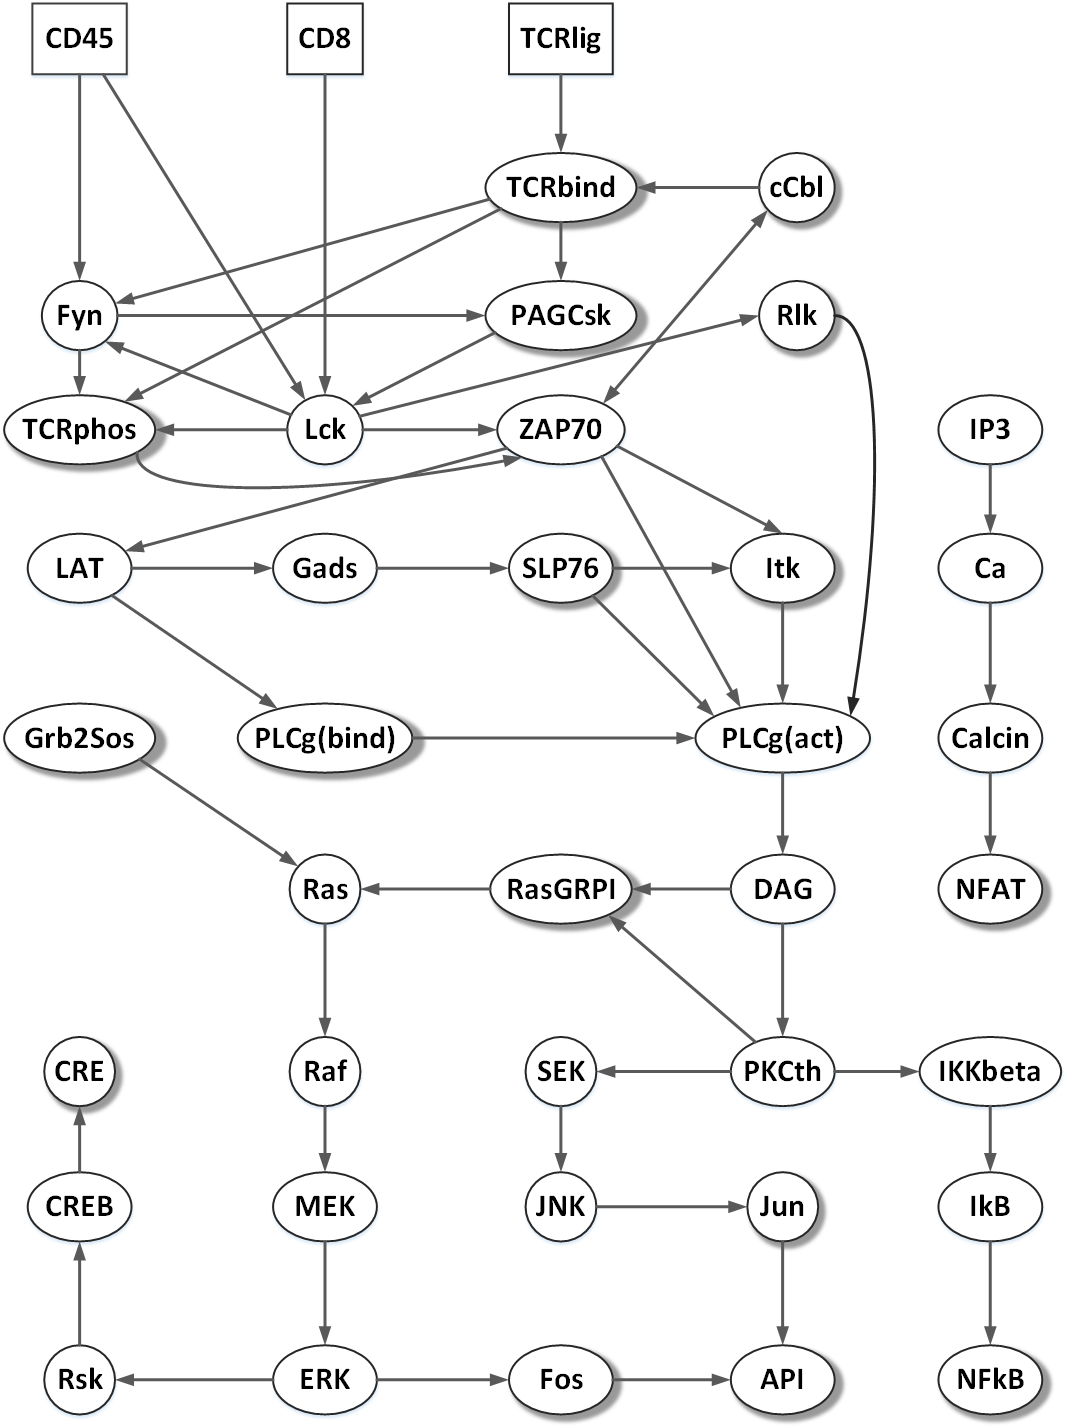
\includegraphics[scale=0.277]{/Fig6.png}}
	%}}
      
     % \caption{Schematic interaction diagram. f = free ligand; b = TCRs
%bound to ligand; k = receptor-associated PTK activity; x = tyrosine
%kinase-dependent inhibitory pathway; s = metabolic and mitogenic
%response. Positive and negative interactions are indicated by a plus and
%minus sign, respectively.}
  %    \label{fig:6}
  %\end{figure}

As the wide application of \BCNs, there are a lot of research work about the control-theoretic problems of \BCNs. The work in \cite{Akutsu2007Control} proves that the problem of determining the controllability of \BCNs\ is {\em NP}-hard in the number of nodes. In addition, it points out that ``One of the major goals of systems biology is to develop a control theory for complex biological systems.'' Since then, the study on control-theoretic problems in the areas of \BNs\ and \BCNs\ has drawn great attention \cite{cheng2009controllability, Zhao2010Input, Cheng2011Identification, Cheng2011Analysis,Fornasini2013Observability}. What is more, the controllability and observability are the basic control-theoretic problems of \BCNs. % Among these studies, \emph{semi-tensor product} (\STP) is one of useful tools to deal with  both \BNs\ and \BCNs\  related problems \cite{cheng2009controllability}.  We will refer to \STP\ in the {\em Section \ref{sec:pre}}. Moreover,  the concept of \BCN\'s observability was proposed firstly in \cite{cheng2009controllability}. 

However, in this paper we research the observability of the \BCNs. The concept of observability was proposed firstly in \cite{cheng2009controllability}. To date, there are four types of observability have been proposed. And they are mainly about how to get some information of the initial value of the state-nodes of the \BCNs\ by the value of their input-nodes and output-nodes. Because the value of state-nodes can be reflected by the value of output-nodes. Moreover, the value of state-nodes at the next time step is affected by the value of state-nodes and input-nodes. Such that we can control and predict the new value of the state-nodes by the value of input-nodes. Therefore, with the updating rules of \BCNs\ we get some information about the initial value of state-nodes of \BCNs\ by the value of input-nodes and output-nodes. Then based on actual application needs, different types of observability are defined to get different kinds of information about the initial value of state-nodes%Therefore, we can get some information about the initial state $s_0$ by the output of the \BCN.
%If there are multipal type of initial state $s_0$ of a \BCN\ with the same output $o_0$, then we can not determine the initial state by the initial output. 
% Then, we can use the input to control the state of \BCNs, and then get more information about the new state by the new output we observed. So that, we can get more information about the initial state of \BCN\ by controlling the input.

For convenience, we use the vectors input $i$, state $s$ and output $o$ to represent the value of the input-nodes, state-nodes and output-nodes of a \BCN\ respectively. Then an input sequence $i_0, i_1,\ldots, i_{p-1}$ consists of several inputs in sequential time steps, a state sequence $s_0, s_1,\ldots, s_{p-1}$ consists of several states in sequential time steps, and an output sequence $o_0, o_1,\ldots, o_{p-1}$ consists of several outputs in sequential time steps. Such that, for the initial state $s_0$ of a \BCN\ and its input sequence $i_0, i_1,\ldots, i_{p-1}$, we have a corresponding state sequence $s_0, s_1,\ldots, s_{p}$ and a corresponding output sequence $o_0, o_1,\ldots, o_{p}$ for this \BCN.

As we mentioned before, there are four types of observability have been proposed. The four existing observability of \BCNs\ are as follows.
%A output can be seen as a vector of the values of all output-nodes of the \BCN\ in a time step as well. Therefore a output sequence also consists of several outputs in sequential time steps. 
%Moreover,  \cite{cheng2009controllability} gives equivalent conditions for controllability of \BCNs\ and observability of controllable \BCNs. 
\begin{enumerate}
	\item The first type of observability proposed in 2009 \cite{cheng2009controllability}, and it means that every initial state $s_0$ can be determined by an input sequence $i_0, i_1,\ldots, i_{p-1}$. Such that, as we inputing $i_0, i_1,\ldots, i_{p-1}$, the corresponding output sequence ($o_0, o_1,\ldots, o_{p}$) of $s_0$ is different from the corresponding output sequence of any other types of initial state. Therefore, we can distinguish the $s_0$ from other types of initial state by this input sequence, and then we can determine whether the initial state is $s_0$ by this input sequence.
	\item 
	The second observability proposed in 2010 \cite{Zhao2010Input}, and it is determined in \cite{Li2015Controllability}. It stands that for every two distinct initial states $s_0$ and $s_0'$, there exists an input sequence $i_0, i_1,\ldots, i_{p-1}$ which can distinguish them. Such that, as we inputing $i_0, i_1,\ldots, i_{p-1}$, the corresponding output sequences ($o_0, o_1,\ldots, o_{p}$, $o_0', o_1',\ldots, o_{p}'$) of them are different from each other. Therefore, we can distinguish between these two types of initial state $s_0$ and $s_0'$ by the corresponding input sequence.	
	\item The third observability proposed in 2011 \cite{Cheng2011Identification}, and it states that there is an input sequence $i_0, i_1,\ldots, i_{p-1}$ that determines the initial state $s_0$. Such that, the corresponding output sequence of all types of initial state are different. Therefore, we can determine the initial state of the \BCN\ by this input sequence for every initial state.
	
	\item  The fourth observability proposed in 2013 \cite{Fornasini2013Observability} is essentially the observability of linear control systems, i.e., every sufficient long input sequence $i_0, i_1,\ldots, i_{p-1}$ can determine the initial state $s_0$. Such that, the corresponding output sequence of any types of initial state are different. Therefore, we can determine the initial state of the \BCN\ by every sufficient long input sequence for every initial state.
\end{enumerate}
 
%\tl{can you state the four types observability clearly and formally here?}

%\rev{****input s equence***}

In {\em Section \ref{sec:pre}}, we will present the formal definition of four observability completely and introduce their implication relationship% in the following pages. What's more, there is an approach to study large-scale \BCNs\ via network aggregations \cite{Zhang2017Observability}. In order to further improve the performance of the \BCN\ model, we make some optimizations about the definition of observability of \BCNs.     which can be checked at most once

In the four existing observability, we can not determine the initail state of \BCNs\ in real time by the first and second observability. Although we can determine the initail state of \BCNs\ in real time by the third and fourth observability, the requirements for \BCNs\ to determine the initail state are very harsh. Thus, we consider that whether we can determine the initial state of some \BCNs\ which can not be determined by the third and fourth observability.

In the porcess determining the initial state, we infer the set of possible initial states $S_k$ by observing the output of \BCN\ at every time step $k$. The input $i_k$ we chose should make every two distinct states (${s_k}^i$, ${s_k}^j$ ) in the set of possible initial states will not turn into be the same state after affected by $i_k$. And the new set of possible initial states $S_{k+1}$ is derived by the input $i_k$ we chose and the new output $o_{k+1}$ we observe at the time step $k+1$, and we have $|S_{k+1}|\le|S_k|$. If $|S_{k+1}|=1$, we can determine the initial state $s_0$ of the \BCN.

What's more, in the third and fourth observability, if a \BCN\ satisfies the observability there has to exist an input sequence that determines its initial state $s_0$. But we can also determine the set of possible initial states $S_0$ by initial output $o_1$ we observe, and then we use different input sequences to determine initial state ($s_0\in S_0$) for different sets of possible initial states. In this case, the requirements for \BCNs\ to determine the initail state would be less harsh because we utilize the set of possible initial states $S_0$ to find the input sequence. Then we propose the online observability in this paper wich means that we find input sequence by the $S_k$, where $S_k$ is the set of initail states derived at every time step $k$. With the online observability, we can determine the initial state of some \BCNs\ which can not be determined before.

% With the output we observed at every time step, we can further determine the range of the initial state. As we can further determine the range, we can use different input sequence to determine the initial state. However, in the third and fourth existing observability, we have to use the same input sequence to determine the initial state without utilizing the range of the initial state. In this paper, we propose the concept of online observability which determine the initial state by making full use of the input and output of \BCNs. With the online observability, we can determine the initial state of some \BCNs\ which can not be determined before.
%we do not utilize the range of the initial state to derive the input at every time step. In the online observability, we make full use of the input and output of \BCNs\ to determine their initial state. 

In the online observability, we make full use of the input and output of \BCNs\ at every time step to determine their initial state. Therefore, a \BCN\ is online observable iff we can determine its initial state $s_0$ in real time for every initial state $s_0$. Comparing with the existing first and second observability, the online observability has the {\em real-time} property because we can determine the initial state in real time. However, comparing with the existing third and fourth observability, it has {\em interactivity} that we would make full use of the input and output of a \BCN\ to determine its initial state. With the {\em real-time} property and {\em interactivity}, we call this type of observability online observability. %In the porcess determining the initial state, we infer the set of possible initial states by observing the output of \BCN\ ar every time step. And then, we choose the input that every two distinct states in the possible initial states will not turn into be the same state after affected by this input. With the set of possible initial states, we can choose one input to refine the possible initial states set in the time step $k+1$. We repeat above procedure until the cardinality of initial states set turns into be one then we can determine the initial state of \BCNs. That is why we call this process a dynamic process. 

In order to study online observability better, we formulate the formal definition for it. Firstly, we define the derivation function to describe the derivation process of the state of \BCNs\ by their output and input at every time step. Secondly, we propose the definition of the $K$-step determinability to present that we can use a set of possible current states to determine the current state of \BCNs\ in real time in finite time steps. The derivation function and $K$-step determinability are all preparations for defining the the online observability. Thirdly, we define the online observability that for every set of possible states which derived at the time step $0$, it satisfy $K$-step determinability. By the definition, we prove that online observability is the necessary and sufficient condition of determine the initial state of \BCNs\ in real time for every initial state. Finally, we compare the online observability with existing four observability. That the online observability implies the first and second observability but not imply the third and fourth observability.

After we defined the online observability and campred it with with existing four observability, we propose two algorithms to determine it. The first one is the supertree-based algorithm, the supertree of a \BCN\ intuitively depicts how to derive the state of the \BCN\ by alternately observing the output and then deriving and deciding the input untill we can determine the state of \BCN. But there are some shortcomings in this algorithm, so we propose the algorithm based on directed graph. In the algorithm based on directed graph, we check whether the $K$-step determinability of the sets with less possible states and then check the sets with more possible states. So that, it can help us find all paths to determine the initial state of \BCNs.

Finally, in order to further illustrate the advantages of the online observability, we present how to use it to do some optimization in the process of determining the initial state. The first one is to find the shortest path and the second one is to avoid entering critical states. It because that the {\em interactivity} let the online observability has better performance than existing observability in the dynamic analysis of \BCNs.

In conclusion, in this paper we make the following contributions. 
%The four  types of observability  have many nice properties that they can be used in some useful applications. However, all of the four types of observability of \BCNs\ are offline observability which means that they can not adjust the input sequence by observing the output sequence in the process of determining the initial state of \BCNs. This property of offline observability limits the performance of \BCNs. In order to further improve the performance of \BCNs, we propose the online observability that we can determine the initial state of \BCNs\ dynamically. In other words,  the online observability decides the input sequence in each time step by observing the out sequence. In the  online observability, we infer the possible  initial states set by observe outputs of \BCN\ in the first $k$ time steps. Through the  possible  initial states, we can choose one input to refine the possible initial states set in the time step $k+1$. We repeat above procedure until the cardinality of initial states set turns into be one then we can determine the initial state of \BCNs. That is why we call this process a dynamic process. 
%In the porcess determining the initial state, we derive and decide the input in each time step by observing the out.


\subsubsection*{Contributions}
Firstly, we propose and formally define the concept of online observability of \BCNs. Comparing with existing observability, the online observability can help to determine the initial state of some biological systems. Secondly, in addition to theoretical research, we also provide two algorithms to determine the online observability for \BCNs. Finally, we present some optimization brought by the online observability of \BCNs. Including methods to find shortest path and approaches to avoid entering critical states in the process of determining the initial state of \BCNs.  These optimization further explain the advantages of online observability of \BCNs. %\rev{No important points}%\rev{***Compare with offline observabilities****} 

Then the remainder of this paper is organized as follows.
\subsubsection*{Structure}
 {\em Section \ref{sec:pre}} introduces necessary preliminaries about \BCNs, algebraic forms of \BCNs\ and the four existing types of observability of  \BCNs. {\em Section \ref{sec:online}} presents the definition of derivation function, $k$ steps determinability and online observability of \BCNs. {\em Section \ref{sec:deter}} presents how to determine the online observability of \BCNs\ by super tree and directed graph. {\em Section \ref{sec:app}} talks about some applications of the online observability of \BCNs. We also compare the online observability with offline observability in this section. {\em Section \ref{sec:con}} ends up  with the introduction of our future work.

%\tl{I will try to rewrite the intro.}

%==============================================================================================================


% !Mode\dots ``TeX:UTF-8''
% !TEX root = ../bare_jrnl.tex
\section{Preliminaries} 
\label{sec:pre}
In this section we introduce the definition of \BCNs\ and their algebraic forms, as well as the four existing types of observability. 

$\mathbb{B}$ : the set $\{0,1\}$; $t=0,1,\ldots$ represents the discrete time. 

\subsection{Boolean Control Networks}

A Boolean control network can be defined as a directed graph together with logical equations to describe the updating rules of the nodes of the directed graph. The formal definition of \BCN\ is given as follows. 

\begin{definition}[Boolean Control Networks, \cite{Ideker2001A}] A \BCN\ consists of the  topology and the associated updating rules. The topology is captured by a directed graph which consists of input-nodes, state-nodes, output-nodes, and directed edges which connect nodes. 
	\begin{itemize}
	\item Every node in a \BCN\ can take a logic value from $\{0,1\}$ at a discrete time $t=0, 1, 2,\ldots$ 
	
	\item Every directed edge from a state-node $s_1$ (or an input-node $i_1$) to a state-node $s_2$ means that the logic value of $s_2$ at time step $t+1$ is affected by the logic value of $s_1$ (or $i_1$)  at time step $t$. 
	
	\item Every directed edge from a state-node $s_1$ to an output-node $o_1$ means that the logic value of $o_1$ at time step $t$ is affected by the logic value of $s_1$  at time step $t$.  
	\end{itemize}

Assuming that the \BCN\ has $n$ state-nodes, $m$ input-nodes and $q$ output-nodes. Then the updating rules of the \BCN\ can be described as following formulas:
\begin{equation}
\begin{split}
s(t+1)=&f(i(t),s(t))\\
o(t)=&h(s(t))
\end{split}
\label{equ:1}
\end{equation}
where
\begin{itemize}
	\item $s(t)\in \mathbb{B}^n$ is a state which represent the logic value of all state-nodes at time step $t$; 	
	\item $i(t)\in \mathbb{B}^m$ is a input which represent the logic value of all input-nodes at time step $t$; 	
	\item $o(t)\in \mathbb{B}^q$ is a output which represent the logic value of all output-nodes at time step $t$;  
	\item $f:\mathbb{B}^{n+m}\mapsto \mathbb{B}^n$ and $h:\mathbb{B}^n\mapsto \mathbb{B}^q$ are logical functions that represent the updating rules of the {\em BCN}. 
	\end{itemize}
%Where $\mathbb{B}$ : the set $\{0,1\}$; $t=0,1,\ldots$ represents the discrete time. 
 

\end{definition}

In order to better illustrate the definition of BCN, we give an example as follows.

%Note that one can only know that whether a node is affected by another node from the network graph. Different \BCNs\ may have the same structure, in order to determine a \BCN\ uniquely, 

 
 \begin{figure}[thpb]
      \centering
      \framebox{\parbox{3in}{
		\centerline{\includegraphics[scale=0.23]{Fig1}}
	}}
      
      \caption{A Boolean control network with two input-nodes $A$ and $B$, four state-nodes $C$, $D$, $E$ and $F$, and two output-nodes $G$, $W$. We use blue, black and orange, to distinguish three types of nodes and three types of edges.}
      \label{fig:1}
  \end{figure}

%To better illustrate the concept of {\em BCNs}, we give a simple example to describe it.

\begin{example}
In Fig.\ref{fig:1} we have a \BCN\ with two input-nodes $A$ and $B$, four state-nodes $C$, $D$, $E$ and $F$, two output-nodes $G$, $W$ and the directed edges which connect them. And we have the updating rules of this \BCN\ that \[C(t), D(t), E(t), F(t)\in s(t)\] denote the value of state-nodes at time step $t$;
\[A(t), B(t)\in i(t)\] denote the value of input-nodes at time step $t$;
\[G(t), W(t)\in o(t)\] denote the value of output-nodes at time step $t$;
$f:\mathbb{B}^{6}\mapsto \mathbb{B}^4$ and $h:\mathbb{B}^4\mapsto \mathbb{B}^2$ are shown in the truth table (Fig.\ref{fig:2}).  For instance, the updating rule of output-node $G$ is 
\[G(t)=C(t)\wedge \neg(\neg{D(t)}\wedge \neg E(t)\wedge \neg F(t)).\]
%\[C(t+1)=(A(t)\wedge B(t))\vee (C(t)\wedge D(t))\vee (E(t)\wedge F(t))\]
The reason why we use the truth table to describe the updating rules of the \BCN\ is that it would be will be more convenient for a \BCN\ to be converted into its aglebraic form. What's more, for convenience, we will use this example to explain various concepts throughout this paper.
  \begin{figure}[thpb]
      \centering
      \framebox{\parbox{3in}{
		\centerline{\includegraphics[scale=0.26]{Fig2.png}}
	}}
      
      \caption{The truth table which describe the updating rules of the \BCN\ shown in Fig.\ref{fig:1}.}
      \label{fig:2}
   \end{figure}
   \label{exa:2}
\end{example}   


%==============================================================================================================
\subsection{The algebraic forms of \BCNs}
As mentioned in the {\em Section \ref{sec:intro}}, \STP\ is one of useful tools to deal with  both \BNs\ and \BCNs\  related problems \cite{cheng2009controllability}. The \STP\ is used to represent the algebraic form of \BCN. The algebraic form of \BCN\ helps us to introduce four existing observability of \BCN\ and define the online observability of \BCN. The definition of \STP\ is as follows.

\begin{definition}[STP] 
	\cite{Cheng2011Analysis} Let $X\in\mathbb{R}_{m\times n}$, $Y\in\mathbb{R}_{p\times q}$ and $\alpha=lcm(n,p)$ be the least common multiple of $n$ and $p$. The \STP\ of $X$ and $Y$ is defined as \[X\ltimes Y=(X\otimes I_{\alpha/n})(Y\otimes I_{\alpha/p}),\] where $\otimes$ denotes the {\em Kronecker product}. 
\end{definition}

After introducing the definition of \STP\ of matrices,  we introduce some related notations at first \cite{Zhang2016Observability}:
\begin{itemize}
  \item $\delta^i_n$: the $i$-th column of the identity matrix $I_n$;
  \item $\Delta_n$: the set $\{\delta^1_n,\ldots,\delta^n_n \}$; 
  \item $\delta_n \left[i_1,\ldots,i_s\right]$: $\left[\delta^{i_1}_n,\ldots,\delta^{i_s}_n\right]\left(i_1,\ldots,i_s\in\left\{1,2,\ldots,n\right\}\right)$ the logical matrix;
  \item  $L_{n\times s}$: the set of $n\times s$ logical matrices.
\end{itemize}

Using \STP\ of matrices, the updating rules of the \BCN\ (\ref{equ:1}) can be quivalently represented in the following algebraic form:
\begin{definition}

\begin{equation}
\begin{split}
s(t+1)=&\ L\ltimes{i(t)}\ltimes{s(t)}\\
o(t)=&\ H\ltimes{s(t)}
\end{split}
\label{equ:2}
\end{equation}
where $s(t)\in\Delta_N$, $i(t)\in\Delta_M$, and  $o(t)\in\Delta_Q$ denote the states, inputs and outputs respectively the same as in formula (\ref{equ:1}), but $s(t)$, $i(t)$ and $o(t)$ in formula (\ref{equ:2}) written with the special vector forms; $L\in L_{N\times\left(NM\right)}$ and $H\in L_{Q\times N}$ denote the relation matrices, where $N=2^n$, $M=2^m$, and $Q=2^q$. 
\end{definition}

Since \STP\ keeps most properties of the conventional product \cite{Cheng2011Analysis}, the associative law, the distributive law, etc., we usually omit the symbol ``$\ltimes$'' hereinafter. For instance, the 
formula \[s(t+1)=L\ltimes{i(t)}\ltimes{s(t)}\] will be written as  \[s(t+1)=L{i(t)}{s(t)}.\]

After the introduction of the algebraic forms of \BCNs, we introduce the process of constructing a \BCN\' s algebraic form. In order to construct the algebraic form of \BCN\ (\ref{equ:2}) we give a mapping \[\tau:\{0,1\}\mapsto \{\delta_2^1, \delta_2^2\},\] where $\tau(0)=\delta_2^2$, $\tau(1)= \delta_2^1$. 
%each logical value a vector form as: $1 \scriptsize{\sim} \delta_2^1$, $0 \scriptsize{\sim} \delta_2^2$. 
Therefore, the logical variable $A(t)$ takes value from these two vectors, i.e., $A(t)\in \{\delta_2^1, \delta_2^2\}$. Using the \STP\ of matrices, we have 
\[i(t)=i_1(t){\ldots}i_m(t);\] 
\[s(t)=s_1(t){\ldots}s_n(t);\] 
\[o(t)=o_1(t){\ldots}o_q(t).\] 
And according to \cite{Cheng2003Semi}, for the logical function of each state-node $f_p$ which can be found in the updating rules (\ref{equ:1}) that
\[f_p(i_1(t),\ldots,i_m(t),s_1(t),\ldots,s_n(t)),\] 
there exists a logical matrix $L_p\in L_{2\times {NM}}$ such that
\begin{equation}
\begin{split}
\tau(f_p(i_1(t),\ldots,i_m(t),s_1(t),\ldots,s_n(t)))= L_pi(t)s(t)
\end{split}
\end{equation}
%where the left side of equation calculate the truth value and the  right side of equation calculate the vector in $\{\delta_2^1, \delta_2^2\}$. 
Therefore for state-nodes $s_1,\ldots,s_n$, we have $n$ logical matrices $L_1,\ldots,L_n$ for them, respectively. 
%We have that
%when\\
If for each state-node $s_p$ the logical matrix has its form
\[L_p=[\delta_2^{p_1},\ldots,\delta_2^{p_{NM}}],\] 
then we have that %for the set of all state-nodes $s(t)$ the logical matrix 
\[L=[\delta_N^{R_1},\ldots,\delta_N^{R_{NM}}]\]  where 
\[\delta_N^{R_1}=\delta_2^{1_1}\ldots\delta_2^{n_1};\]\[\vdots\] \[\delta_N^{R_{NM}}=\delta_2^{1_{NM}}\ldots\delta_2^{n_{NM}}.\] 

%then 

By this relationship we can construct the $L$ for the algebraic forms of \BCNs. What's more we can also construct the logical matrix $H$ in the similar way. To better illustrate the concept of algebraic forms, we give a simple example to describe it.
\begin{example}
For instance, for the \BCN\ mentioned in {\em Example \ref{exa:2}}, we have that the updating rules of this \BCN\ can be represented with the algebraic form:
\begin{equation}
\begin{split}
s(t+1) =&\delta_{16}[\alpha]i(t)s(t)\\
o(t) =&\delta_4[\beta]s(t)\\
\end{split}
\label{equ:4}
\end{equation}
where $\alpha=\{10,4,11,16,9,5,1, 7,15,2,3,12,7,6,8,13,8,9,\\15,10,14,4,3,16,1,14,12,13,5,7,2,6,7,2,3,13,13,9,5,1,\\16,13 ,6,14,11,10,4,15,1,14 ,7,6,9 ,8,11,12,5,5,13,3,10,\\12,16,16\}$, $\beta=\{1,1,1,2,2,2,2,3,3,3,3,4,4,4,4,4\}$, $t\in \mathbb{N}$, $s\in \Delta_{16}$, $i\in \Delta_4$ and $o\in \Delta_4$.
\end{example}   
\subsection{Four existing observability of \BCNs}
After introducing the algebraic forms of \BCNs, we introduce four existing types of observability of \BCNs\ in this subsection. In order to introduce four existing types of observability of \BCNs, we define the mappings \cite{Zhang2016Observability}:
\begin{equation}
\begin{split}
L^p_{s_0} &: (\Delta_M)^p\mapsto(\Delta_N)^p, i_0\ldots i_{p-1} \mapsto s_1 \ldots\, s_p\\
L^{\infty}_{s_0} &: (\Delta_M)^{\infty}\mapsto(\Delta_N)^{\infty}, i_0 i_1 \ldots  \mapsto s_1 s_2 \ldots
\end{split}
\label{equ:5}
\end{equation}
\begin{equation}
\begin{split}
(HL)^p_{s_0} &: (\Delta_M)^p\mapsto(\Delta_Q)^p, i_0\ldots i_{p-1} \mapsto o_1\ldots\, o_p\\
(HL)^{\infty}_{s_0} &: (\Delta_M)^{\infty}\mapsto(\Delta_Q)^{\infty}, i_0 i_1 \ldots  \mapsto o_1 o_2\ldots
\end{split}
\label{equ:6}
\end{equation}

Where $\Delta_N$, $\Delta_M$ and $\Delta_Q$ are three alphabets, $s_0\in \Delta_N$, $p\in \mathbb{Z}_+$ and $\infty$ is the infinite natural numbers. For all  $p\in \mathbb{Z}_+$, \[I=i_0 \ldots i_{p-1} \in(\Delta_M)^p\] is an input sequence, \[L^p_{s_0}(I)=s_1 \ldots s_{p} \in(\Delta_N)^p\] is a state sequence and \[(HL)^p_{s_0}=o_1 \ldots o_{p} \in(\Delta_N)^p\] is a output sequence. For the $\infty$, \[I=i_0 \ldots  \in(\Delta_M)^{\infty}\] is an infinitely long input sequence, \[L^{\infty}_{s_0}(I)=s_1 \ldots  \in(\Delta_N)^{\infty}\] is an infinitely long state sequence and \[(HL)^{\infty}_{s_0}(I)=o_1 \ldots \in(\Delta_N)^{\infty}\] is an infinitely long output sequence. From the algebraic forms of \BCNs, in the formula (\ref{equ:5}), for any $1\le k \le |I|$ we have \[s_k=Li_{k-1}s_{k-1}.\] In the formula (\ref{equ:5}) and formula (\ref{equ:6}), for any $1\le k \le |I|$ we have  \[o_k=Hs_k=HLi_{k-1}s_{k-1}.\] 

Then four existing types of observability of BCNs can be defined as follows.
%And for all $1\ge k \ge j \ge |I|$, we use I[k,j] to denote the word $i_k \ldots i_j$ as an input sequence. 
\begin{definition}
The first type of observability is that, a \BCN\ is called observable, if for every initial state $s_0 \in \Delta_N$, there exists an input sequence $I\in(\Delta_M)^p$ for some $p\in \mathbb{Z}_+$ such that for every two states $s_0\neq {s'}_0\in \Delta_N$, $Hs_0=H{s'}_0$ implies $(HL)^p_{s_0}(I)\neq (HL)^p_{{s'}_0}(I)$ \cite{cheng2009controllability}.
\end{definition}

Hence the first observability means that if a \BCN\ is observable then every initial state of the \BCN\ can be determined by an input sequence. But we can only use the corresponding input sequence $I_i$ of a state $s_i$ to check whether the state $s_i$ is the initial state $s_0$ of this \BCN\ or not.
\begin{example}
For example, for the \BCN\ mentioned in {\em Example \ref{exa:2}}, we have for every initial state of this \BCN\ can be determined by an input sequence.  For instance,
\begin{itemize}
  \item the state $\delta_{16}^1$ can be determined by any input sequence which with the prefix $\delta_{4}^4$, $\delta_{4}^1 \delta_{4}^3$ or $\delta_{4}^1 \delta_{4}^4$, etc;
  \item the state $\delta_{16}^2$ can be determined by any input sequence which with the prefix $\delta_{4}^1$, $\delta_{4}^3$ or $\delta_{4}^4$, etc;
  \item the state $\delta_{16}^2$ can be determined by any input sequence which with the prefix $\delta_{4}^2$, $\delta_{4}^4$ or $\delta_{4}^1 \delta_{4}^4$, etc.
\end{itemize} 

Therefore we have this \BCN\ satisfies the existing first observability.
\end{example}   

\begin{definition}
	The second type of observability is that, a \BCN\ is called observable if for any distinct states $s_0$, ${s'}_0 \in \Delta_N$, there exists an input sequence $I\in(\Delta_M)^p$ for some $p\in \mathbb{Z}_+$, such that $Hs_0=H{s'}_0$ implies $(HL)^p_{s_0}(I)\neq (HL)^p_{{s'}_0}(I)$ \cite{Zhao2010Input}.
\end{definition}

The second observability means that a \BCN\ is called observable if for every two distinct initial states $s_0, s_0'$of the \BCN, there exists an input sequence $I$ which can distinguish them. 
\begin{example}
For example, for the \BCN\ mentioned in {\em Example \ref{exa:2}}, we have for every two distinct initial states of the \BCN, there exists an input sequence which can distinguish them.  For instance,
\begin{itemize}
  \item the states $\delta_{16}^1$ and $\delta_{16}^2$ can be distinguished by any input sequence which with the prefix $\delta_{4}^1$, $\delta_{4}^2 \delta_{4}^1$ or $\delta_{4}^2 \delta_{4}^2$, etc;
  \item the states $\delta_{16}^1$ and $\delta_{16}^3$  can be distinguished by any input sequence which with the prefix $\delta_{4}^2$, $\delta_{4}^3$ or $\delta_{4}^4$, etc;
  \item the states $\delta_{16}^2$ and $\delta_{16}^3$  can be distinguished by any input sequence which with the prefix $\delta_{4}^1$, $\delta_{4}^2$ or $\delta_{4}^4$, etc.
\end{itemize} 

Therefore we have this \BCN\ satisfies the existing second observability.
\end{example}   
\begin{definition}
The third type of observability is that, a \BCN\ is called observable if there exists an input sequence $I\in(\Delta_M)^p$ for some $p\in \mathbb{Z}_+$, such that for any distinct states $s_0$, ${s'}_0 \in \Delta_N$, $Hs_0=H{s'}_0$ implies $(HL)^p_{s_0}(I)\neq (HL)^p_{{s'}_0}(I)$ \cite{Cheng2011Identification}.
\end{definition}

The third observability means that a \BCN\ is called observable if there exists an infinitely long input sequence which can determine the initial state $s_0$ of the \BCN\ for every $s_0\in\Delta_N$.

\begin{example}
For example, for the \BCN\ mentioned in {\em Example \ref{exa:2}}, we have there is an input sequence which can determine the initial state of this \BCN.  For instance, any input sequence which with the prefix $\delta_{4}^1\delta_{4}^4\delta_{4}^1$ can determine the initial state $s_0$ of the \BCN\ for every $s_0\in\Delta_N$.

Therefore we have this \BCN\ satisfies the existing third observability.
\end{example}  
\begin{definition}
	The fourth type of observability is that, \BCN\ is called observable, if for any distinct states $s_0$, ${s'}_0 \in \Delta_N$, for any input sequence $I\in(\Delta_M)^{\infty}$, $Hs_0=H{s'}_0$ implies $(HL)^{\infty}_{s_0}(I)\neq (HL)^{\infty}_{{s'}_0}(I)$ \cite{Fornasini2013Observability}.
\end{definition}

The fourth observability means that a \BCN\ is called observable if every sufficient long input sequence can determine the initial state $s_0$ of the \BCN\ for every $s_0\in\Delta_N$.
\begin{example}
For example, for the \BCN\ mentioned in {\em Example \ref{exa:2}}, we have there exists at least one sufficient long input sequence that can not determine the initial state of this \BCN. For instance, the states $\delta_{16}^4$ and $\delta_{16}^5$  will convert into $\delta_{16}^{13}$ after being affected by $\delta_{4}^3$, therefore any input sequence which with the prefix $\delta_{4}^3$, they can not determine the initial state $s_0$ of the \BCN\ for every $s_0\in\Delta_N$.

Therefore we have this \BCN\ does not satisfy the existing fourth observability.
\end{example}  

What is more, we know the implication relationships of four existing types of observability from the definitions of them \cite{Zhang2016Observability}. 

 \begin{figure}[thpb]
      \centering
      \framebox{\parbox{3in}{
		\centerline{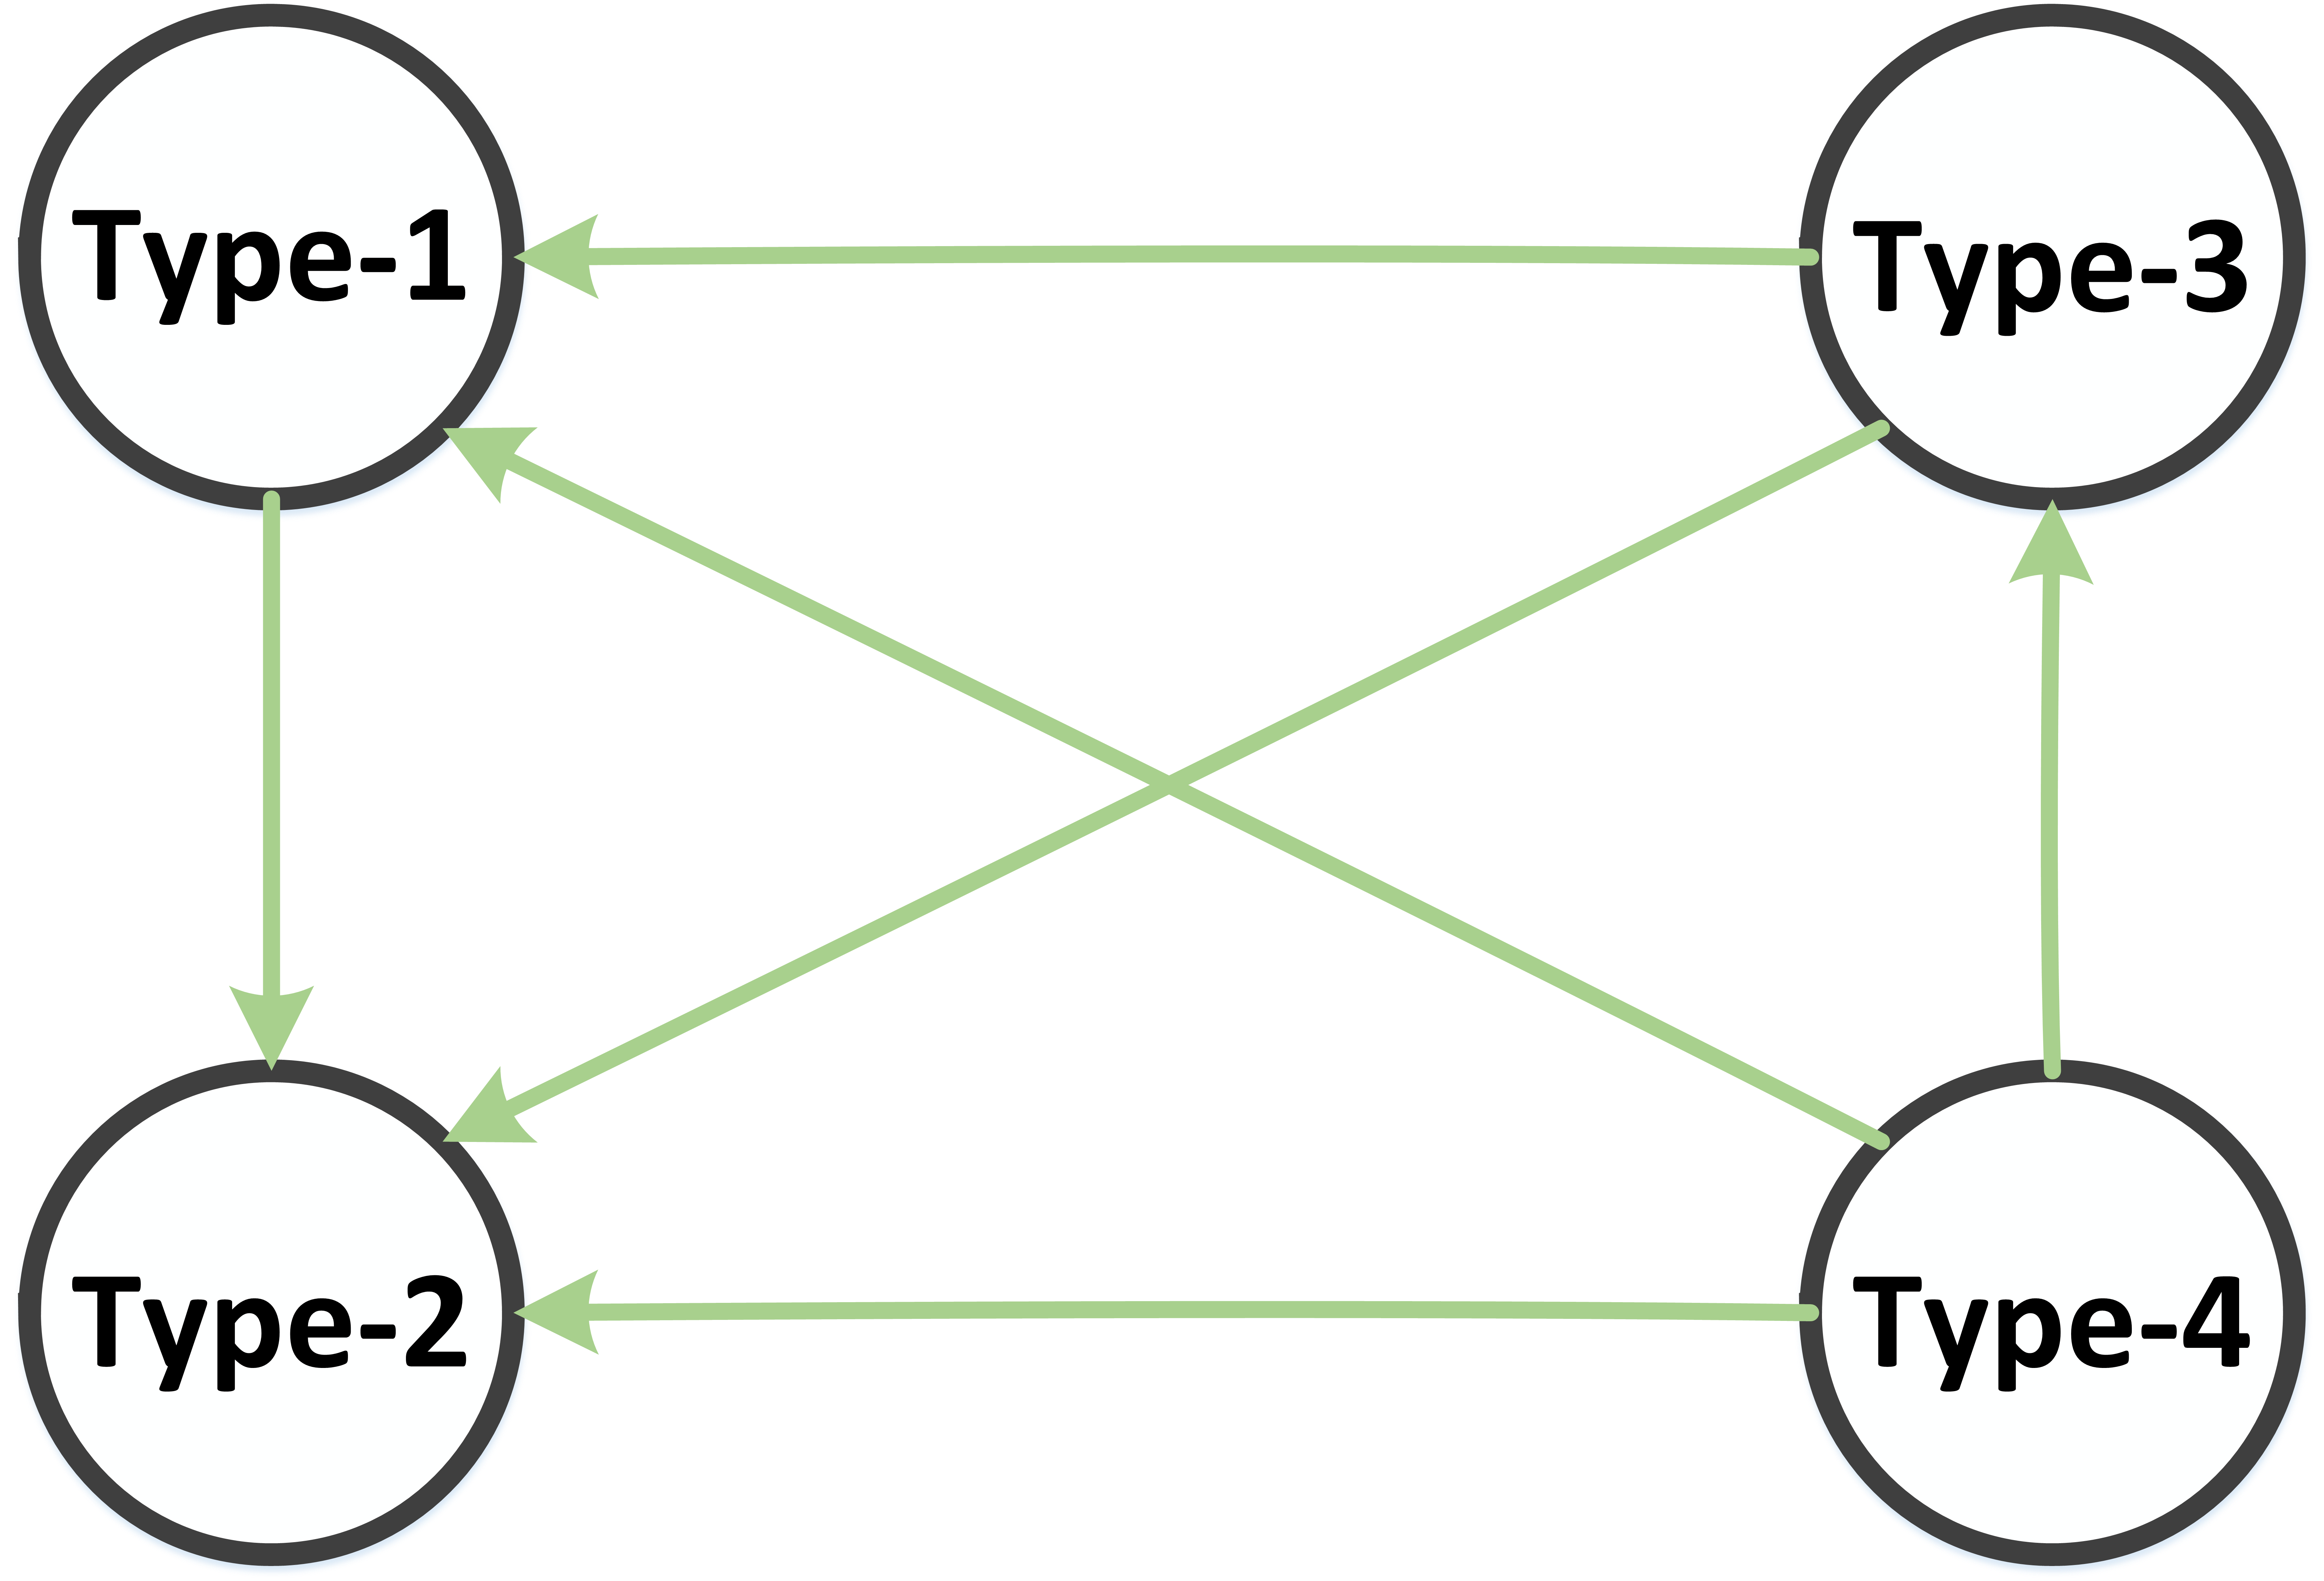
\includegraphics[scale=0.27]{Fig9.png}}
	}}
      
      \caption{The implication relationships graph between existing observability 1, 2, 3, 4, where ``$\rightarrow$" means ``implies".}
      \label{fig:9}
   \end{figure}
%\begin{proposition}
%The implication relationships of four existing types of observability.
%\begin{itemize}
%\item The first observability implies the second observability, but the second observability does not imply the first observability.\\
%\item The third observability implies the second observability, but the second observability does not imply the third observability.\\
%\item The third observability implies the first observability, but the first observability does not imply the third observability.\\
%\item The fourth observability implies the third observability, but the third observability does not imply the fourth observability.\\
%\item The fourth observability implies the second observability, but the second observability does not imply the fourth observability.\\
%\item The fourth observability implies the first observability, but the first observability does not imply the fourth observability. \\
%\end{itemize} 
%\end{proposition}

Where the implication relationship is that ``The first observability implies the second observability.'' means ``If a \BCN\ satisfies the first observability then it satisfies the second observability.'' For the details of the proving process of this proposition, we refer readers to \cite{Zhang2016Observability}.
%, when we don't presuppose the initial state of {\em BCNs}
   
After introducing the definition of four existing observability and their implication relationship, we discuss how to determine the initial state of some \BCNs\ in real time by four existing types of observability. 
\begin{itemize}
\item The first and second observability can not help us to determine the initial state of some \BCNs\ in real time. Because in the first observability we need to assume that the initial state $s_0$ of a \BCN\ is $s_i$, and then check it by corresponding input sequence $I_i$ of this state. If the initial state we assume is correct, then we can determine the initial state $s_0=s_i$. But if the assumption is not correct, we can not determine the initial state of the \BCN. Therefore we need to check several test cases (with the same initial state $s_0$) of this \BCN\ untill we can determine the initial state of them. So do the existing second observability of \BCNs.
\item We can use the third existing observability and fourth existing observability to determine the initial state of \BCNs\ in real time, because we do not need to presuppose the initial state. But the requirements for \BCNs\ are very harsh when we use the third observability and fourth observability. Because we do not make full use of the output and input in the process of determining the initial state. The output of \BCNs\ we observed at every time step can help us further determine the range of the initial state. Then we can use different input sequence to determine the initial state based on the range of the initial state. However, in the third and fourth existing observability, we have to use the same input sequence to determine the initial state.
\end{itemize} 
 
In some biological systems (depicted by \BCNs), the initial state of them can be checked at most once, i.e., we can only check the initial state of some biological systems in real time. Therefore, we can not use the first observability and second observability to determine the initial states of them in real time. Moreover, in some biological systems, it would takes many costs to check these biological systems. Hence we will spend a lot of overhead to determine the initial states of them by the first observability and second observability. Furthermore, we also can not use the third observability and fourth observability to determine the initial states of some biological systems if they do not satify the requirements of the third and fourth observability. With these disadvantages of four existing observability, we propose the online observability of \BCNs\ to solve this problem.
 \subsubsection*{Problem}
Finding the necessary and sufficient condition of determine the initial state $s_0$ of \BCNs\ in real time for every $s_0\in \Delta_N$.

% !Mode\dots ``TeX:UTF-8''
% !TEX root = ../root.tex
\section{The online observability of \BCNs}
\label{sec:online}
In this section we propose the online observability to solve the problem mentioned before, and we will introduce its related information in detail. 
%\begin{definition}
	 %In the online observability we determine the state of \BCN\ by observing its output sequence and then deriving and deciding the input sequence at every time step. What is more, this process can be accomplished in finite time steps.
%\end{definition}  without presupposing the initial state of \BCN

\ly{In the existing third and fourth observability, there has to exist an input sequence that determines its initial state $s_0$ if a \BCN\ satisfies the observability. }
But we can reduce the scale of  set of possible initial states $S_0$  after we obtain the initial output $o_1$ at time step $0$, and then we find input sequence to determine initial state ($s_0\in S_0$) for different sets of possible initial states. These input sequences can be different, and we can also determine the initial state of the \BCN.
In this case, the requirements for the \BCN\ to determine the initail state would be less harsh since we utilize the set of possible initial states $S_0$ to find the input sequence. Furthermore, if we utilize the sets of possible initial states $S_0$ and $S_1$ derived in time step $0$ and $1$ to find the input sequence to determine the initail state, the requirements for \BCNs\ would further less harsh. According to this law, in the online observability we find input sequence by the $S_t$ we derive at every time step, such that the requirements would be least harsh. Thus, a \BCN\ satisfies the online observability iff its initial state $s_0$ can be determined in real time for every $s_0 \in \Delta_N$.

The reason why we called this type of observability online observability is as follows.
\begin{itemize}
  \item Firstly, in the online observability, we determine the initial state of \BCNs\ in real time. In other words, we only need one test case to determine the initial state of \BCNs. We call this property {\em real-time} property.%Such that we can determine the initial state of any test case of \BCNs.
  \item  Secondly, in the online observability, we use the outputs we observe to derive and decide the input sequence at every time step in the process of determining the initial state of \BCNs. By this way, we can make full use of the outputs and inputs to determine the initial state of \BCNs. We call this property {\em interactivity}.
\end{itemize} 

%We need the {\em real-time} property to help us avoid repeating biological experiments, and the {\em real-time} property makes the online observability be the sufficient condition of determine the initial state $s_o$ of \BCNs\ in real time. However, the {\em interactivity} would help us to find the necessary condition by making full use of the outputs and inputs to determine the initial state of \BCNs. 
With the  {\em real-time} and {\em interactivity}, we called this type of observability online observability.
%\tl{maybe I did not understand this, but I think you are confusing two things: the observability and the algorithm (approach) to determine the initial state. It seems to me that you are describing a new approach (the online approach), but does this change the observability? if yes, how? Is this a stronger notion or a weaker notion or incomparable?}

%The observability we propose can determine the initial state online.
 %Because in the process of determining the initial state every input of the input sequence is decided by the output we observe at every time step. 
After introducing the properties of the online observability, we briefly present how to determine the initial state of \BCNs\ in real time. At every time setp $t$, we observe the output $o_t$ of \BCNs, then we can infer the set of possible states $S_t$ by the output $o_t$ at first. %Then as we can know the possible states set
Secondly, with the set of possible states $S_t$ we can derive the set of possible inputs $I_t$, such that for every $i_t\in I_t$ we have that $s_i, s_j$ will not turn into the same state after being affected by the input $i_t$ i.e., $Ls_i i_t\neq Ls_j i_t$ for any distinct $s_i, s_j\in S_t$. This principle will be shown in the equation (\ref{equ:12}). And then, we choose an input from $I_t$. Thirdly, the set of possible initial states $S_{t+1}$ of next time step is derived by the input $i_t$ we chose and the new output $o_{t+1}$ we observe. The cardinal number of possible states set $|S_{t+1}|$ does not change or decrease in this process shown in the equations (\ref{equ:9}) and (\ref{equ:10}). If the cardinal number of new possible states set $|S_{t+1}|$ turn into be $1$ then we can determine the state and the initial state of \BCN. 

Therefore, in the definition of online observability, firstly we need to describe how to derive the set of possible states of the \BCN\ by the output and input in every time step. So we define the derivation function to solve this problem. Secondly, we need to describe whether we can use a set of possible states determine the inistial state  in real time for every $s_0 \in \Delta_N$ by the above mentioned process, then we define the $K$-step determinability. 

Therefore, we have the definition of the online observability that if for a \BCN\ every set possible states we derived at time step $0$ satisfies $K$-step determinability, then it is online observable.

 In the left of this section, firstly we define derivation function. Secondly we present the definition of $k$-step determinability (before $K$-step determinability). Thirdly, we give the formal definition of the online observability of \BCNs\ by derivation function and $K$-step determinability. Finally, we compare the online observability with four existing observability.
\subsection{Derivation function}
%Different from four existing observabilities, t

 
 % After deciding input, we can observe the new output, and then we can infer the new possible states set.
In order to better describe how to derive the set of possible states $S_k$ and the set of possible inputs $I_k$ at every time step $k$, we propose the derivation function. The definition of this function is as follows.
\begin{definition}[Derivation Function] The derivation function can be defined as $\Ded\left(S, i, o\right)$. Based on derivation process mentioned before, we have that there exists the corresponding $s'\in S$ of $s$ such that 
%\[s=L\ltimes i\ltimes s'\ when\ i\neq \varepsilon, \] 

\[s=\left\{
\begin{array}{rcl}
L\ltimes i\ltimes s'      &      & {i\neq \varepsilon}\\
s'       &      & {i= \varepsilon}
\end{array} \right. \]

and 

\[H\ltimes s=o\ when\ o\neq \varepsilon, \]
for each element \[s\in \Ded\left(S, i, o\right)\]
\end{definition}
where   
\begin{itemize}
  \item $S\in 2^{\Delta_N}$ is the possible states set;
  \item $i\in (\Delta_M\cup\varepsilon)$ represents the input;
  \item $o\in(\Delta_Q\cup\varepsilon)$ represents the output; 
  \item $\Ded\left(S, i, o\right)\in 2^{\Delta_N}$ is the possible states set determined by derivation function.
\end{itemize} 
 
 We can get the set of states $\Ded\left(S, i, o\right)$ for $S$ after inputing $i$ and observing $o$ by this function. Moreover, we have some equations for this function. For better illustration, we will use the \BCN\ mentioned in {\em Example \ref{exa:2}} as an example. And we can know the details of this function better by researching these equations.
\begin{equation}
\begin{split}
\Ded\left(\emptyset,i,o\right)=\emptyset\\
%D\left(\varnothing,I_i,O_i\right)=D\left(\varnothing,\varepsilon,O_i\right)= &D\left(\varnothing,\varepsilon,\varepsilon\right)=\varnothing\\
\end{split}
\label{equ:7}
\end{equation}

Equation (\ref{equ:7}) represents that if the possible states set is an empty set of states $\emptyset$, then no matter what we input and observe we can only deduce the possible set is the empty set $\emptyset$. It means that if we don't know anything about the state of a \BCN, then we can not deduce anything no matter what we do.
\begin{equation}
\begin{split}
\Ded\left(S,\varepsilon,\varepsilon\right)=&S\\
\end{split}
\label{equ:8}
\end{equation}

 In equation (\ref{equ:8}), we have that for any possible states set $S$, and we neither input anything nor observe the output. In this case we can only deduce that the possible states set is $S$. It means that we can not know more information about a \BCN\ than what I knew before before observing the output and deciding the input of this \BCN.
\begin{equation}
\begin{split}
\Ded\left(\Delta_N,\varepsilon,\delta_4^1\right)=&\{\delta_{16}^1,\delta_{16}^2,\delta_{16}^3\}\\
\end{split}
\label{equ:9}
\end{equation}
 
In equation (\ref{equ:9}). When the possible states set $S=\Delta_N$, and  we observe that the outputs of \BCN\ is $\delta_4^1$ before we decide input. In this case we can derive that the possible states would be $\delta_{16}^1$, $\delta_{16}^2$ or  $\delta_{16}^3$. This equation shows how to derive the set of possible states by observing the output at every time step. So we have that the cardinal number of the possible states set may decrease after we observing the output of \BCN. As the cardinal number of the set possible states decreases, we can further determine the range of values for the initial state. And it would help us derive the set possible inputs. Therefore, the derivation function would make the online obervability satisfy the {\em interactivity}.
\begin{equation}
\begin{split}
\Ded\left(\{\delta_{16}^1,\delta_{16}^2,\delta_{16}^3\},\delta_4^1,\varepsilon\right)=&\{\delta_{16}^{10},\delta_{16}^4,\delta_{16}^{11}\}\\
\end{split}
\label{equ:10}
\end{equation}

And then, if the possible states set $S=\{\delta_{16}^1$, $\delta_{16}^2$, $\delta_{16}^3\}$ and we input $\delta_4^1$. Before we observe the output of the \BCN\ we can only derive that the possible states would be $\delta_{16}^{10}$, $\delta_{16}^4$ or  $\delta_{16}^{11}$ shown in equation (\ref{equ:10}). In other words, the cardinal number of the possible states set does not decrease before observing the output of this \BCN. Therefore the input $\delta_4^1$ is a suitable input, this equation shows how to derive the set of possible inputs.
\begin{equation}
\begin{split}
\Ded\left(\{\delta_{16}^4,\delta_{16}^5,\delta_{16}^6\},\delta_4^3,\varepsilon\right)=&\{\delta_{16}^9,\delta_{16}^{13}\}
\end{split}
\label{equ:12}
\end{equation}

 Finally if the set of possible states is $\{\delta_{16}^4,\delta_{16}^5,\delta_{16}^6\}$ and the inputs is $\delta_4^3$. Before we observe the output of \BCN\ we can derive that the possible states should be $\delta_{16}^9$ or $\delta_{16}^{13}$ shown in equation (\ref{equ:12}). Because both $\delta_{16}^4$ and $\delta_{16}^5$ are turn into be the same state $\delta_{16}^9$ after affected by $\delta_4^3$. And if the current state of the \BCN\ is one of them then we can not determine the  state any more. Therefore, the derivation function helps us define the online obervability to satisfy the {\em real-time} property. 
 
 We give a lemma to to better illustrate the {\em real-time} property.
\begin{lemma}
 At time step $k$, $S$ is the set of current possible states we derived and $i(k)$ is the input we chose. If we can determine the current state $s(k)$ of this \BCN\ in real time for every $s(k)\in S$, then we have 
 $|\Ded\left(S,i(k),\varepsilon\right)|=|S|$.
 \label{lemm:1}
\end{lemma}

\begin{proof}
At time step $k$, $S$ is the set of current possible states we derived and $i(k)$ is the input we chose. And we can determine the current state $s(k)$ of this \BCN\ in real time for every $s(k)\in S$. 

Firstly, we assume that $|\Ded\left(S,i(k),\varepsilon\right)|<|S|$. Then we have that there are two possible states $s_i(k), s_j(k)\in S$, $s_i(k)\neq s_j(k)$ such that 
\[s_i(k+1)=L\ltimes i(k)\ltimes s_i(k)=L\ltimes i(k)\ltimes s_j(t)=s_j(k+1).\]
And then for any $p\in \mathbb{N}^*$ we have 
\[s_i(k+p)=s_j(k+p);\]
\[o_i(k+p)= H\ltimes{s_i(k+p)}= H\ltimes{s_j(k+p)}=o_j(k+p).\]
 Therefore we can not distinguish between $s_i(k)$ and $s_j(k)$ any more.
 If the current state $s(k)$ is one of the two possible states $s_i(k)$ and $s_j(k)$, then we can not determine the $s(k)$ in real time. 
 
 But we have that we can determine the current state $s(k)$ of this \BCN\ in real time for every $s(k)\in S$, then the presumption $|\Ded\left(S,i(k),\varepsilon\right)|<|S|$ is wrong, thus $|\Ded\left(S,i(k),\varepsilon\right)|=|S|$.
\end{proof}
 
% If the cardinality number of the possible states set of one \BCN\ decreased before observing its output the derivation process, then we can not deduce its initial state any more i.e., we can not determine the initial state of this \BCN\ any more. Therefore, the derivation function helps the online obervability satisfy the {\em real-time} property. 

 At time step $k$ and $S$ is the set of current possible states we derived. As the derivation function can only describe the derivation process the set of possible states $S$ and the set of possible inputs of the \BCN\ at a time step. But we need to know how to choose the input at every time step to determine the initial state of the \BCN\ in real time. Thus we propose the $k$-step determinability for the set of possible states $S$ to depicted whether we can determine the initial state in real time.
\subsection{$k$-step determinability}
After we difined the derivation function, we present the definition of $k$-step determinability for the set of states $S$, where the $k\in \mathbb{N}$.% It may easier to difine online observability by programming language. But we would like to define its mathematical form for preciseness of concepts. However, before defining the online observability of \BCNs, we need to difine the $k$-step determinability of the states set of \BCNs\ at first.
\begin{definition}[$k$-Step Determinability] 

When $k=0$, a set of states $S$ the $S$ is $0$-step deterministic iff the cardinal number of this states set $|S|=1$. 

When $k>0$, a set of states $S$ is $k$-step deterministic
 iff the cardinal number of this states set $|S|>1$ and for this set of states $S$ there exists $i_p \in \Delta_M$ such that
 \begin{itemize}
 \item  $|\Ded\left(S,i_p,\varepsilon\right)|=|S|$, and 
 \item  for each $o_j$ in $\Delta_Q$ such that $|\Ded\left(S,i_p,o_j\right)|\neq 0$, there exists a ${k'}<k$ such that $\Ded\left(S,i_p,o_j\right)$ is $k'$-step deterministic.
 \end{itemize}
 %And we default $k\ge0$ when we talk about whether a states set of \BCNs\ $S$ is $k$-step deterministic or not.
\end{definition}

 In the time step $t$ and $S$ is the set of current possible states we derived. If $k=0$, from the definition of {\em$k$}-step determinability we know that the cardinality number of possible states set  $|S|=1$, then we can determine the current state of the \BCN. Therefore we can determine the state without deriving and deciding any input and observing output in ``$k=0$'' step. If $k>0$, we have $|S|>1$. Guided by the {\em Lemma \ref{lemm:1}}, we use the formula $|\Ded\left(S,i_p,\varepsilon\right)|=|S|$ to ensure that no different states will turn into be the same state after being affected by the input $i_p$. Without this formula, we can not guarantee that the current state $s(t)$ can be determined in real time for every $s(t)\in S$. Furthermore, for each $o_j$ in $\Delta_Q$ such that $|\Ded\left(S,i_p,o_j\right)|\neq 0$ there exists a ${k'}<k$ that $\Ded\left(S,i_p,o_j\right)$ is $k'$-step deterministic, it make sure that we can can determine the initial state in real time. The $k$-step deterministic ( $k>0$) is defined recursively, and it requires the definition of $0$-step deterministic.

 In order to better illustrate this definition, we give the following example.
\begin{example}
In the \BCN\ mentioned in {\em Example \ref{exa:2}}. For the set of state $\{\delta_{16}^1,\delta_{16}^2,\delta_{16}^3\}$, the cardinality number of this set $|\{\delta_{16}^1,\delta_{16}^2,\delta_{16}^3\}|=3>1$, and for this set there exists $\delta_{4}^4$ such that 
 \begin{itemize}
 \item  $|\Ded\left(\{\delta_{16}^1,\delta_{16}^2,\delta_{16}^3\},\delta_{4}^4,\varepsilon\right)|=|\{\delta_{16}^1,\delta_{16}^2,\delta_{16}^3\}|$;
 \item  $|\Ded\left(\{\delta_{16}^1,\delta_{16}^2,\delta_{16}^3\},\delta_{4}^4,\delta_{4}^1\right)|=|\{\delta_{16}^1\}|=1$, and $\{\delta_{16}^1\}$ is $0$-step deterministic;
 \item  $|\Ded\left(\{\delta_{16}^1,\delta_{16}^2,\delta_{16}^3\},\delta_{4}^4,\delta_{4}^2\right)|=|\{\delta_{16}^7\}|=1$, and $\{\delta_{16}^7\}$ is $0$-step deterministic;
  \item  $|\Ded\left(\{\delta_{16}^1,\delta_{16}^2,\delta_{16}^3\},\delta_{4}^4,\delta_{4}^4\right)|=|\{\delta_{16}^14\}|=1$, and $\{\delta_{16}^14\}$ is $0$-step deterministic.
 \end{itemize}
 Therefore the set of states $\{\delta_{16}^1,\delta_{16}^2,\delta_{16}^3\}$ is $1$-step deterministic.
\end{example}  

In addition, we propose some lemma for the $k$-step determinability.
\begin{lemma}
 In the time step $t$ and $S$ is the set of current possible states we derived. If $S$ is $k$-step deterministic, then we can determine the current state $s(t)$ of this \BCN\ for every $s(t)\in S$ in real time at time step ($t+k$).
  \label{lemm:6}
\end{lemma}
\begin{proof} If $k=0$, then we have $|S|=1$. Therefore, we can determine the current state $s(t)$ of this \BCN\ in real time at time step $t$, and then the {\em Lemma \ref{lemm:6}} is right. 

If for $k=0,\ldots k=p$ the {\em Lemma \ref{lemm:6}} is right. When $k=p+1$ and the $S$ is $k$-step deterministic, then we have for this set of states $S$ there exists $i_p \in \Delta_M$ such that
 \begin{itemize}
 \item  $|\Ded\left(S,i_p,\varepsilon\right)|=|S|$, and 
 \item  for each $o_j$ in $\Delta_Q$ such that $|\Ded\left(S,i_p,o_j\right)|\neq 0$ there exists a ${k'}<(p+1)$ that $\Ded\left(S,i_p,o_j\right)$ is $k'$-step deterministic.
 \end{itemize}
 However, for $k=0,\ldots k=p$ the {\em Lemma \ref{lemm:6}} is right, thus we can determine the state $s(t+1)$ of this \BCN\ for every $s(t+1)\in \Ded\left(S,i_p,\varepsilon\right)$ in real time at time step $(t+1+k')$. What is more, we have $|\Ded\left(S,i_p,\varepsilon\right)|=|S|$, then for every $s(t+1)\in \Ded\left(S,i_p,\varepsilon\right)$ we can find the corresponding one $s(t)$ for it. So we can determine the state $s(t)$ of this \BCN\ for every $s(t)\in S$ in time step $(t+p+1)$. So we have if for $k=0,\ldots k=p$ the {\em Lemma \ref{lemm:6}} is right then the {\em Lemma \ref{lemm:6}} is right too when $k=p+1$. 
 
The {\em Lemma \ref{lemm:6}} is right when $k=0$, and if for $k=0,\ldots k=p$ the {\em Lemma \ref{lemm:6}} is right then the {\em Lemma \ref{lemm:6}} is right too when $k=p+1$. Thus we have the {\em Lemma \ref{lemm:6}} is right for any $k\in \mathbb{N}$.
\end{proof}

The {\em Lemma \ref{lemm:6}} indicates that for the set of current possible states $S$ we derived, $S$ is $k$-step deterministic is the sufficient condition of determine the current state $s(t)$ of this \BCN\ for every $s(t)\in S$ in real time at time step ($t+k$). Therefore, the $k$-step determinability helps us define the online obervability to satisfy the {\em real-time} property. 
\begin{lemma}
 In the time step $t$ and $S$ is the set of current possible states we derived. If we can determine the current state $s(t)$ of this \BCN\ for every $s(t)\in S$ in real time in time step $t+k$, then $S$ is $k$-step deterministic. 
  \label{lemm:7}
\end{lemma}

\begin{proof}
If $k=0$ and we can determine the current state $s(t)$ of this \BCN\ for every $s(t)\in S$ in time step $t$. So we have $|S|=1$, and then $S$ is $0$-step deterministic. Therefore, we have the {\em Lemma \ref{lemm:7}} is right when $k=0$. 

If for $k=0,\ldots k=p$ the {\em Lemma \ref{lemm:7}} is right. When $k=p+1$ and we can determine the current state $s(t)$ of this \BCN\ for every $s(t)\in S$ in real time in time step $t+k$, then from the {\em Lemma \ref{lemm:1}} we have for this set of states $S$ there exists $i_p \in \Delta_M$ such that $|\Ded\left(S,i_p,\varepsilon\right)|=|S|$. And $s(t+1)$ can be determined in time step $(t+1+p)$ for every $s(t+1)\in \Ded\left(S,i_p,\varepsilon\right)$. Then we have that for each $o_j$ in $\Delta_Q$ such that $|\Ded\left(S,i_p,o_j\right)|\neq 0$ there exists a ${k'}<(p+1)$ that $\Ded\left(S,i_p,o_j\right)$ is $k'$-step deterministic.
Therefore, we have $S$ is $(p+1)$-step deterministic. And then have if for $k=0,\ldots k=p$ the {\em Lemma \ref{lemm:7}} is right then the {\em Lemma \ref{lemm:7}} is right too when $k=p+1$. 

The {\em Lemma \ref{lemm:7}} is right when $k=0$, and if for $k=0,\ldots k=p$ the {\em Lemma \ref{lemm:7}} is right then the {\em Lemma \ref{lemm:7}} is right too when $k=p+1$. Thus we have the {\em Lemma \ref{lemm:7}} is right for any $k\in \mathbb{N}$.
\end{proof}

The {\em Lemma \ref{lemm:7}} indicates that for the set of current possible states $S$ we derived, $S$ is $k$-step deterministic is the necessary condition of determine the current state $s(t)$ of this \BCN\ for every $s(t)\in S$ in real time at time step ($t+k$). Therefore, the $k$-step determinability helps us define the online obervability to satisfy the {\em interactivity}. 
%Therefore if we can determine the infimum of $k$ for a set of states $S$, we would find the length of the shortest path to determine the state of a \BCN\ by this possible states set $S$.
\begin{lemma}
 If a set of states $S$ is $k_1$-step deterministic and $k_1< k_2$, then $S$ is $k_2$-step deterministic. But if the states set $S$ is $k_1$-step deterministic and $k_1> k_2$, we can not deduce that $S$ is $k_2$-step deterministic. 
  \label{lemm:2}
\end{lemma}

\begin{proof}
 A set of states $S$ is $k_1$-step deterministic and the $k_1< k_2$. 
 
 If $k_1=0$ then $|S|=1$. Therefore for this set of states $S$ there exists $i_p$ in $\Delta_M$ such that
 \begin{itemize}
 \item  $|\Ded\left(S,i_p,\varepsilon\right)|=|S|=1$, and 
 \item  for each $o_j$ in $\Delta_Q$ such that $|\Ded\left(S,i_p,o_j\right)|\neq 0$ and $\Ded\left(S,i_p,o_j\right)$ is $k'$-step deterministic and ${k'}=0=k_1< k_2$.
 \end{itemize}
 Therefore the set of states $S$ is $k_2$-step deterministic.
 
 If $k_1>0$, then $|S|>1$. Therefore for this set of states $S$ there exists $i_p$ in $\Delta_M$ such that
 \begin{itemize}
 \item  $|\Ded\left(S,i_p,\varepsilon\right)|=|S|$, and 
 \item  for each $o_j$ in $\Delta_Q$ such that $|\Ded\left(S,i_p,o_j\right)|\neq 0$ and $\Ded\left(S,i_p,o_j\right)$ is $k'$-step deterministic and ${k'}<k_1< k_2$.
 \end{itemize}
 Therefore the set of states $S$ is $k_2$-step deterministic.

 But if the states set $S$ is $k_1$-step deterministic and $k_1> k_2$. What is more, for this set of states $S$ there is no such $i_p$ in $\Delta_M$ such that
 \begin{itemize}
 \item  $|\Ded\left(S,i_p,\varepsilon\right)|=|S|$, and 
 \item  for each $o_j$ in $\Delta_Q$ such that $|\Ded\left(S,i_p,o_j\right)|\neq 0$ and $\Ded\left(S,i_p,o_j\right)$ is $k'$-step deterministic with  ${k'}<k_2<k_1$.
 \end{itemize}
 Therefore the set of states $S$ is not $k_2$-step deterministic.
 
 So we have the {\em Lemma \ref{lemm:2}} is right.
\end{proof}
From the {\em Lemma \ref{lemm:2}}, we know that the exists the infimum of $k$ for the $k$-step determinability of a set of states $S$, which indicate the shortest path to definitely determine the state of a \BCN\ by this possible states set $S$ in real time.
\begin{definition}[$k_{inf}(S)$] 
If for a set of states $S$, there exists a $k_i\in \mathbb{N}$ such that $S$ is $k_i$-step deterministic but $S$ is not $(k_{i}-1)$-step deterministic, then $k_{i}$ is the $k_{inf}(S)$ of $S$.
\end{definition}

In {\em Section \ref{sec:app}}, we will represent the details on how to find the shortest path when we use the online observability to determine the initial state of a \BCN. And some other some other advantages of the online observability.

%{\em Theorem \ref{theo:4}}

%We can consider ``A set of possible states $S$ is $K$-step deterministic'' as ``We can determine the state of a \BCN\ by this possible states set $S$ in finite steps''. Therefore we have some other theorems for the $K$-step determinability.



%We prove the {\em Lemma \ref{lemm:4}} at first.
\begin{lemma}
 If a set of states $S_j$ is $k$-step deterministic and $S_i\subset S_j$, then $S_i$ is $k$-step deterministic, where $|S_j|>1$.
  \label{lemm:4}
\end{lemma}
\begin{proof}
A set of states $S_j$ is $k$-step deterministic and $S_i\subset S_j$, where $|S_j|>1$. Therefore we have $k>0$ from this precondition.

If $k=1$, we have for this set of states $S_j$ there exists $i_p$ in $\Delta_M$ such that
 \begin{itemize}
 \item  $|\Ded\left(S_j,i_p,\varepsilon\right)|=|S_j|$, and 
 \item  for each $o_j$ in $\Delta_Q$ such that $|\Ded\left(S_j,i_p,o_j\right)|=1$ and $\Ded\left(S_j,i_p,o_j\right)$ is $0$-step deterministic.
 \end{itemize}
 Then we have for the set of states $S_i$ there exists $i_p$ in $\Delta_M$ such that
 \begin{itemize}
 \item  $|\Ded\left(S_i,i_p,\varepsilon\right)|=|S_i|$, and 
 \item  for each $o_j$ in $\Delta_Q$ such that $|\Ded\left(S_i,i_p,o_j\right)|=|\Ded\left(S_j,i_p,o_j\right)|=1$, the $\Ded\left(S_i,i_p,o_j\right)$ is $0$-step deterministic.
 \end{itemize} And then $S_i$ is $1$-step deterministic, thus we have the {\em Lemma \ref{lemm:4}} is right when $k=1$.
 
 If for $k=1,\ldots k=p$ the {\em Lemma \ref{lemm:4}} is right. When $k=p+1$, we have  for this set of states $S_j$ there exists $i_p$ in $\Delta_M$ such that
 \begin{itemize}
 \item  $|\Ded\left(S_j,i_p,\varepsilon\right)|=|S_j|$, and 
 \item  for each $o_j$ in $\Delta_Q$ such that $|\Ded\left(S_j,i_p,o_j\right)|\neq 0$ and $\Ded\left(S_j,i_p,o_j\right)$ is $k'$-step deterministic with  ${k'}<(p+1)$.
 \end{itemize}
 Then we have for the set of states $S_i$ there exists $i_p$ in $\Delta_M$ such that
 \begin{itemize}
 \item  $|\Ded\left(S_i,i_p,\varepsilon\right)|=|S_i|$, and 
 \item  for each $o_j$ in $\Delta_Q$ such that $0\neq |\Ded\left(S_i,i_p,o_j\right)| \le |\Ded\left(S_j,i_p,o_j\right)|$ and $\Ded\left(S_i,i_p,o_j\right)\subset \Ded\left(S_j,i_p,o_j\right)$ is  $k'$-step deterministic with  ${k'}<(p+1)$.
 \end{itemize}  Then we have the $S_i$ is $(p+1)$-step deterministic. Therefore we have if for $k=1,\ldots k=p$ the {\em Lemma \ref{lemm:4}} is right, then the {\em Lemma \ref{lemm:4}} is right too when $k=p+1$. 

The {\em Lemma \ref{lemm:4}} is right when $k=1$, and if for $k=1,\ldots k=p$ the {\em Lemma \ref{lemm:4}} is right then the {\em Lemma \ref{lemm:4}} is right too when $k=p+1$. Thus we have the {\em Lemma \ref{lemm:4}} is right for any $k\in \mathbb{N}^*$.
 
% What is more, we have the {\em Lemma \ref{lemm:4}} is right when $k=1$, thus the {\em Lemma \ref{lemm:4}} is right for every $k\in\mathbb{N}$
\end{proof}

The {\em Lemma \ref{lemm:4}} would help us design the algorithm to determine the online observability of a \BCN, and we will represent the details in the {\em Section \ref{sec:deter}}.

\subsection{Online observability}
After the previous preparation, we present the formal definition of the online observability. The formal definition of the online observability of {\em BCNs} is as follows.

\begin{definition}[Online Observability of  BCNs]
 A \BCN\ is online observable,
iff for every  $o_j \in \Delta_Q$ such that $|\Ded\left(\Delta_N,\varepsilon, o_j\right)|> 0$, the $\Ded\left(\Delta_N,\varepsilon,o_j\right)$ is $K$-step deterministic.
% We even can define the online observability simpler, if there exists $k \ge 0$ implies $\Delta_N$ is $k$ stepes deterministic, then this \BCN\ is online observable. 
\end{definition}

However, since we don not need to find the the specific value of $k$ when we define the online observability, we define the concept of $K$-Step Determinability for convenience.
\begin{definition}[$K$-Step Determinability] 
 In the time step $t$ and $S$ is the set of current possible states we derived. If there exists a $k_i\in \mathbb{N}$ such that $S$ is $k_i$-step deterministic, then the set of states $S$ is $K$-step deterministic.
\end{definition}
%The difference between the second definition and the first definition is that whether we observe the corresponding output of the initial state of \BCN\ at first. For better performance, we use the first definition of online observability.

 In order to better illustrate the definition of online observability, we give the following example.

\begin{example}
In the \BCN\ mentioned in {\em Example \ref{exa:2}}.  We have that:
 \begin{itemize}
 \item $|\Ded\left(\Delta_N,\varepsilon, \delta_{4}^1\right)|=\{\delta_{16}^1,\delta_{16}^2,\delta_{16}^3\}\neq 0$, and this set of states is $1$-step deterministic (also $K$-step deterministic);
 \item $|\Ded\left(\Delta_N,\varepsilon, \delta_{4}^2\right)|=\{\delta_{16}^4,\delta_{16}^5,\delta_{16}^6,\delta_{16}^7\}\neq 0$, and this set of states is $1$-step deterministic (also $K$-step deterministic);
 \item $|\Ded\left(\Delta_N,\varepsilon, \delta_{4}^3\right)|=\{\delta_{16}^8,\delta_{16}^9,\delta_{16}^{10},\delta_{16}^{11}\}\neq 0$, and this set of states is $2$-step deterministic (also $K$-step deterministic);
 \item $|\Ded\left(\Delta_N,\varepsilon, \delta_{4}^4\right)|=\{\delta_{16}^{12},\delta_{16}^{13},\delta_{16}^{14},\delta_{16}^{15},\delta_{16}^{16}\}\neq 0$, and this set of states is $2$-step deterministic (also $K$-step deterministic).
 \end{itemize}
 
Therefore we have this \BCN\ satisfies the online observability.
\end{example}  

From the informal definition and formal definition of online observability, we propose a theorem for the online observability to solve the problem we proposed in the {\em Section \ref{sec:pre}}.
\begin{theorem}
The necessary and sufficient condition of determine the initial state $s_0$ of a \BCN\ for every $s_0\in \Delta_N$ in real time is the online observability of this \BCN. 
\label{theo:1}
\end{theorem}
\begin{proof}
 A \BCN\ is online observable,
then for every  $o_j$ in $\Delta_Q$ such that $|\Ded\left(\Delta_N,\varepsilon, o_j\right)|> 0$, the $\Ded\left(\Delta_N,\varepsilon,o_j\right)$ is $K$-step deterministic. From the {\em Lemma \ref{lemm:6}} we have if the $\Ded\left(\Delta_N,\varepsilon,o_j\right)$ is $K$-step deterministic, then we have there exists a $k_i$ such that we can determine the $s_o$ in real time at time step $k_i$ for every $s_0\in \Ded\left(\Delta_N,\varepsilon,o_j\right)$.  What is more for every  $o_j$ in $\Delta_Q$ such that $|\Ded\left(\Delta_N,\varepsilon, o_j\right)|> 0$, the $\Ded\left(\Delta_N,\varepsilon,o_j\right)$ is $K$-step deterministic. Then we have there exists a $k_j\ge k_i$ such that we can determine the $s_0$ in time step $k_j$ for every $s_0\in \Delta_N$. Therefore we can determine the initial state $s_0$ of \BCNs\ in real time for every $s_0\in \Delta_N$.

If we can determine the initial state $s_0$ of \BCNs\ for every $s_0\in \Delta_N$ in real time, and $\Ded\left(\Delta_N,\varepsilon,o_j\right)$ is the set of possible states we derived at time step $0$. From the {\em Lemma \ref{lemm:7}}, we have for any set of initial possible states $\Ded\left(\Delta_N,\varepsilon,o_j\right)$ we derived, there exists a $k_i$ such that we can determine the $s_o$ in real time at time step $k_i$ for every $s_0\in \Ded\left(\Delta_N,\varepsilon,o_j\right)$. Thus we have  $\Ded\left(\Delta_N,\varepsilon,o_j\right)$ is $k_i$-step deterministic and then  $K$-step deterministic for every  $o_j$ in $\Delta_Q$ such that $|\Ded\left(\Delta_N,\varepsilon, o_j\right)|> 0$. Therefore this \BCN\ is online observable.

So we have the necessary and sufficient condition of determine the initial state $s_0$ of a \BCN\ for every $s_0\in \Delta_N$ in real time is the online observability of this \BCN. 
\end{proof}
%With the online observability we can find the best way we like to determine the initial state of \BCNs.

What is more, we propose some lemma for the $K$-step determinability as well.
\begin{lemma}
 If a set of states $S_j$ is $K$-step deterministic and $S_i\subset S_j$, then $S_i$ is $K$-step deterministic, where $|S_j|>1$.
\label{lemm:3}
\end{lemma}
\begin{proof}A set of states $S_j$ is $K$-step deterministic and $S_i\subset S_j$. Then there exists a $k_i\in \mathbb{N}^*$ such that $S_j$ is $k_i$-step deterministic. By the {\em Lemma \ref{lemm:4}}, we have $S_i$ is $k_i$-step deterministic too, and then the $S_i$ is $K$-step deterministic as well.
\end{proof}

With the {\em Lemma \ref{lemm:3}}, we would have its equivalent proposition is right as well.
\begin{lemma}
 If a set of states $S_i$ is not $K$-step deterministic and $S_i\subset S_j$, then $S_j$ is not $K$-step deterministic. 
  \label{lemm:5}
\end{lemma}
\begin{proof}
A set of states $S_i$ is not $K$-step deterministic and $S_i\subset S_j$. We assume that the set of states $S_j$ is $K$-step deterministic ar first, then we have $S_i$ is $K$-step deterministic too. But $S_i$ is not $K$-step deterministic, therefore we have the assumption is wrong, and then the $S_j$ is not $K$-step deterministic.
\end{proof}

The {\em Lemma \ref{lemm:3}} and {\em Lemma \ref{lemm:5}} help us to determine whether a \BCN\ is online observable in the {\em Section \ref{sec:deter}}.
\subsection{Online observability and existing observability}
After defining online observability of \BCNs, we discuss the implication relationships between four existing observability and online observability. The implication relationship is about the conditions that need to meet these observability. For instance, in the {\em Theorem \ref{theo:2}}, ``The online obervability implies the existing first observability.'' means that ``If a \BCN\ satisfies the online obervability then it satisfies the existing first observability.'' However, ``The existing first observability does not imply the online obervability.'' means that ```A \BCN\ that satisfies the existing first observability does not have to satisfy the online obervability.''

%In the existing first observability, we presuppose the initial state of a \BCN\ at first, and then try to find the input sequence to distinguish it from other types of initial state. But the input sequence determined by the presupposed initial state may make some other types of initial state turn into be the same state (equation \ref{equ:12}). Such that some of other types of initial states can not be distinguished anymore, and if the initial state of this \BCN\ is one of them then the initial state can not be determined anymore. This problem has to be considered in the online obervability of \BCNs. Hence we have a theorem for online observability and the existing first and second observability.
\begin{theorem}
%If a \BCN\ satisfies the online obervability then it satisfies the existing first and second observability. If a \BCN\ satisfies the existing first or second observability we can not deduce that it satisfies the online obervability.
The online obervability implies the existing first observability, but the existing first observability does not imply the online obervability.
\label{theo:2}
\end{theorem}
\begin{proof}
A \BCN\ satisfies the online obervability. From the {\em Theorem \ref{theo:1}} we have that we can determine the initial state $s_0$ of this \BCN\ in real time for every $s_0\in \Delta_N$. Therefore for every initial state $s_0 \in \Delta_N$, there exists an input sequence $I\in(\Delta_M)^p$ for some $p\in \mathbb{Z}_+$ such that the $s_o$ can be determined by the input sequence $I$, and then this \BCN\ satisfies the existing first observability.

However, if a \BCN\ satisfies the existing first observability. What is more there exist two state $s, s'\in\Ded\left(\Delta_N,\varepsilon, o_j\right)$ where $|\Ded\left(\Delta_N,\varepsilon, o_j\right)|> 0$, and the $i_0, i_1,\ldots, i_{p-1}$ is the corresponding one unique input sequences to determine $s$, and the $i'_0, i'_1,\ldots, i'_{p-1}$ is the corresponding one unique input sequences to determine $s'$. If the fitst input of the input sequences $I$ and $I'$ are different, then we can not determine the initial state $s_0$ of this \BCN\ in real time for every $s_0\in \{s,s'\}$. Therefore this \BCN\ does not satisfy the online observability.
\end{proof}

In the existing first observability, we presuppose the initial state of a \BCN\ at first, and then we use its corresponding input sequence to distinguish it from other types of initial state. In other words, we do not consider the {\em real-time} property in the existing first observability which would make the condition more harsh. So we have the online obervability implies the existing first observability, but the existing first observability does not imply the online obervability. Moreover, from the implication relationships between the existing first and second observability which mentioned in the {\em Section \ref{sec:pre}}, we have the implication relationships between the online observability and the existing second observability
\begin{theorem}
%If a \BCN\ satisfies the online obervability then it satisfies the existing first and second observability. If a \BCN\ satisfies the existing first or second observability we can not deduce that it satisfies the online obervability.
The online obervability implies the existing second observability, but the existing second observability does not imply the online obervability.
\label{theo:4}
\end{theorem}
%In the existing third type of observability, there has to exist an input sequence that can distinguish any distinct states. However in online observability we can use different input sequences to distinguish any distinct states in different sets of state. 
%Where these different sets of state are classified by their corresponding outputs. Therefore, we have the existing third type of observability implies the online observability of \BCNs, then the existing fourth type of observability implies the online observability too. 
\begin{theorem}
The online obervability does not imply the existing third observability, but the existing third observability implies the online obervability.
%If a \BCN\ satisfies the existing third or fourth obervability then it satisfies the online observability. But if a \BCN\ satisfies the online obervability, we can neither deduce that it satisfies the third observability nor deduce that it satisfies the fourth observability.
\end{theorem}
\begin{proof}
A \BCN\ is online observable. What is more there are $o,o'\in\Delta_Q$, such that there does not exist $i_p \in \Delta_M$ satisfy that $|\Ded\left(\Ded\left(\Delta_N,\varepsilon, o\right),i_p,\varepsilon\right)|=|\Ded\left(\Delta_N,\varepsilon, o\right)|$ and $|\Ded\left(\Ded\left(\Delta_N,\varepsilon, o'\right),i_p,\varepsilon\right)|=|\Ded\left(\Delta_N,\varepsilon, o'\right)|$. Therefore there does not exist an input sequence $I\in(\Delta_M)^p$ for some $p\in \mathbb{Z}_+$, such that for any distinct states $s_0$, ${s'}_0 \in \Delta_N$, $Hs_0=H{s'}_0$ implies $(HL)^p_{s_0}(I)\neq (HL)^p_{{s'}_0}(I)$. So we have this \BCN\ does not satisfy the existing third observability.

If a \BCN\ satisfies the existing third observability, then there exists an input sequence $I\in(\Delta_M)^p$ for some $p\in \mathbb{Z}_+$, such that for any distinct states $s_0$, ${s'}_0 \in \Delta_N$, $Hs_0=H{s'}_0$ implies $(HL)^p_{s_0}(I)\neq (HL)^p_{{s'}_0}(I)$. And then we can use the input sequence $I$ to determine the initial state $s_0$ of this \BCN\ in real time for every $s_0\in \Delta_N$. So we have this \BCN\ satisfies the online observability.
\end{proof}

In the existing third type of observability, there has to exist an input sequence that can distinguish any distinct states of the \BCN. In other words, we do not consider the {\em interactivity} in the existing third observability which would make the condition less harsh. So we have the online obervability does not imply the existing third observability, but the existing third observability implies the online obervability. Moreover, from the implication relationships between the existing third and fourth observability which mentioned in the {\em Section \ref{sec:pre}}, we have the implication relationships between the online observability and the fourth observability
\begin{theorem}
The online obervability does not imply the existing fourth observability, but the existing fourth observability implies the online obervability.
%If a \BCN\ satisfies the existing third or fourth obervability then it satisfies the online observability. But if a \BCN\ satisfies the online obervability, we can neither deduce that it satisfies the third observability nor deduce that it satisfies the fourth observability.
\label{theo:5}
\end{theorem}

Therefore, the implication relationships graph between four existing observability and online observability is shown in Fig.\ref{fig:7}.
%\begin{example}
%For instance, the \BCN\ whose structure is depicted in Fig.\ref{fig:1}, and the updating rules of this \BCN\ is described as truth table in Fig.\ref{fig:2}. This \BCN\ satisfies the existing first, second, third observability, but it is not satisfy the existing fourth observability. Therefore, we have this \BCN\ satisfies the online observability from the implication relationship between the existing third observability and online observability.
%\end{example}   

\begin{figure}[thpb]
      \centering
      \framebox{\parbox{3in}{
		\centerline{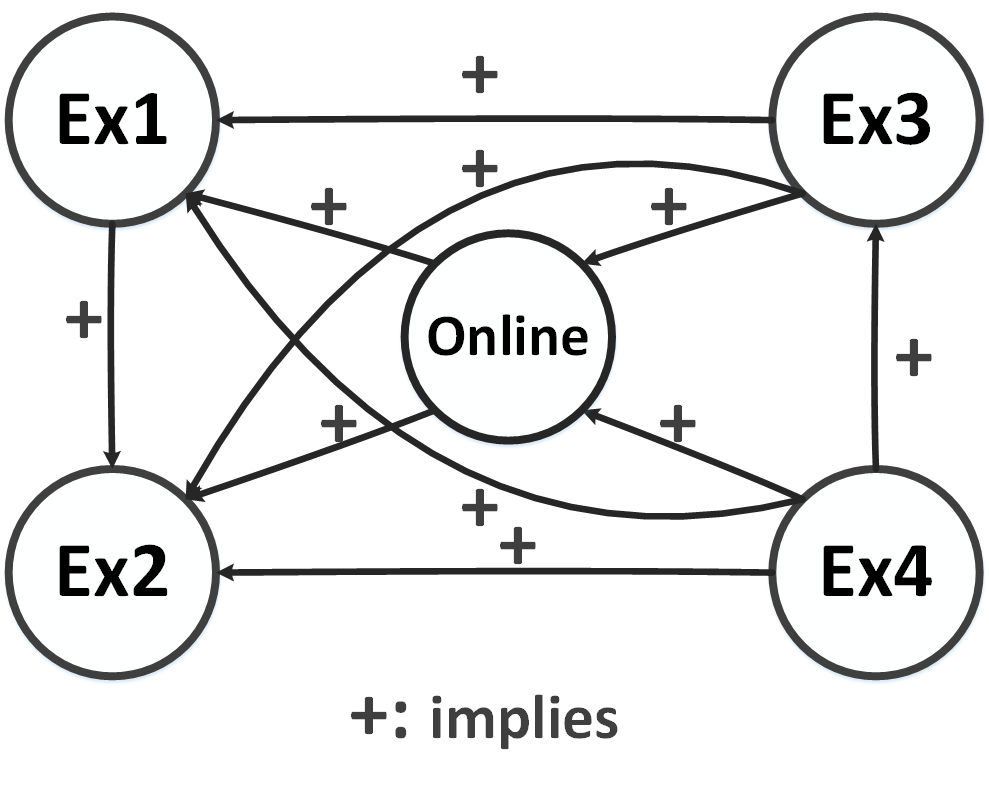
\includegraphics[scale=0.28]{Fig8.png}}
	}}
      
      \caption{The implication relationships graph between existing observability 1, 2, 3, 4, and online observability where ``$\rightarrow$" means ``implies".}
      \label{fig:7}
   \end{figure}

From the implication relationships between online observability and existing observability we know that the online observability can help us solve some problem which can not be solved by existing observability. 
 \begin{itemize}
 \item Firstly, if the systems described by \BCNs\ are online observable but not satisfy the existing third and fourth observability, then the online observability can help us determine their initial state in real time. 
 \item Secondly, it takes least observation costs for us to determine the initial state of some systems described in real time by \BCNs. There are some biological systems depicted by \BCNs, such as the immune systems which can be depicted as the \BCN\ T-cell receptor kinetics model \cite{Klamt2006A}. And there exist input-nodes and state-nodes in this model, for the purpose of obtain the initial state of this \BCN, we must select some state-nodes to be observe at first. However, if we use the online observability of \BCNs\ to determine the initial state of the \BCN\ T-cell receptor kinetics model in real time., then we need least observation costs. 
 \end{itemize}

What is more, with the online observability, we can make some optimizations in the process of determining the initial state. We will represent them in the {\em Section \ref{sec:app}}.
   
   
%When I learned the four existing kinds of observability of \BCNs, I found that if we want to determine the initial state of a \BCN\ by first kind of observability, we need to guess the initial state of the \BCN\ and then check it by its corresponding input sequence. If the initial state we guess is right then we can determine the initial state of this \BCN. But if what we guess is incorrect, we need to guess the initial state again and use its corresponding input sequence to determine the initial state of this \BCN. We repeat this process untll we determine the initial state of this \BCN. But if we can not repeat this process, we can not determine the initial state of the \BCN\ too. Then I turned my gaze to the third observability, this kind of observability makes we can determine the initial state without presupposing the initial state. But I thought if we can determine the possible states set of the \BCN\ by observing the output at first, why do not we find corresponding input sequences for these possible states sets when we determine the initial state of \BCN? Compared with the existing third observability this method needs weaker preconditions of \BCNs\ for us to determine their initial state. Then I talked about this thinkness with my teacher, and we expand it into the original idea of the online observability of \BCNs. 
%==============================================================================================================

% !Mode\dots ``TeX:UTF-8''
% !TEX root = ../root.tex
\section{Determining the online observability of \BCNs}
\label{sec:deter}
After defining the online observability and comparing it with the existing four observability, we propose two algorithms to determine the online observability of \BCNs. The first one is the supertree-based algorithm, and the second one is the algorithm based on directed graph. Based on the definition of online observability, we propose the supertree to describe the process of determining the initial state of a \BCN. And then, we propose the algorithm to determine the online observability of \BCNs\ based on the supertree. But the supertree-based algorithm can not help us find all paths to determine the initial state of a \BCN. In order to improve the shortcomings of the supertree-based algorithm, we propose the algorithm based on directed graph. The algorithm based on directed graph may take longer time for us to determine its online observability. But if we want do some optimizationin in the process of determining the initial state of a \BCN, this algorithm would be better. What is more, we also analyze the complexity of the algorithm based on directed graph in this section. Finally, we represent how to determine the initial state of a \BCN\ by the directed graph.
%The construction processes of supertree and directed graph simulate derivation process of the initial state mentioned before. We check the super tree based on the definition of online observability of \BCNs\ depth first or breadth first. When we find enough leaf nodes, we can make sure the \BCN\ is online observable. But when we use the super tree to find all paths to determine the initial state of a \BCN, we need to check the existence of loops when we build the super tree. And many nodes in the tree are repeated, these nodes will take a lot of time overhead and space overhead for us to build and check the super tree for \BCNs. Therefore, we proposed the second way to determine the online observability of \BCNs\ by using directed graph. By this way we can avoid checking the existence of loop and avoid checking repeated nodes. There are also other advantages which help us select the input better in the process of determining the initial state of a \BCN\ by the second way. All of these advantages will reduce time and space overhead to determine the initial state of a \BCN. In conclusion if a \BCN\ seems to be online observable we would check it earlier by using supertree. But if a  \BCN\ does not seem to be online observable we prefer to check it earlier by using directed graph. If we just want to find a path to determine the initial state of a \BCN\ we would check it by using supertree. But if we want find all paths to determine the initial state of a \BCN\ and make some optimizations in the process of determine the initial state we prefer to check tthe \BCN\ by using directed graph.

\subsection{Supertree-based algorithm} %As we mentioned before, we can use the derivation function to determine the initial state of \BCNs. 
According to the definition of online observability, we alternately observe the output and then derive and decide the input in the process of determining the initial state of a \BCN. When the  cardinal number of the set of possible states comes into be $1$, we can determine the current state of this \BCN\ and then its initial state. We define the supertree for \BCNs\ to describe this process, and then propose the supertree-based algorithm to determine the online observability for \BCNs. For convenience, we use the set of state $S_i$ inside a node to represent this node, and the input $i_p$ or output $o_j$ in an edge to represent the edge.
\begin{definition}[Supertree]
For a \BCN, every node $S_i$ in the supertree is $K$-step deterministic. The root node of its supertree is $\Delta_N$, while the leaf nodes of the supertree are the nodes with cardinal number $1$ ($|S_i|=1$). In addition to the leaf nodes, if a node $S_i$ in the $2k + 1$ ($k\in \mathbb{N}$) layer of the supertree and 
\[|\Ded\left(S_i,\varepsilon, o_j\right)|>0,\]
 then $\Ded\left(S_i,\varepsilon, o_j\right)$ is one of its son nodes, and $o_j$ is the edge from $S_i$ to $\Ded\left(S_i,\varepsilon, o_j\right)$ for each $o_j \in \Delta_Q$. If a node $S_i$ in the $2k+2$ layer of the supertree and  
\[|\Ded\left(S_i,i_p,\varepsilon\right)|=|S_i|,\] 
then $\Ded\left(S_i,i_p,\varepsilon\right)$ is the son node of $S_i$ and $i_p$ is the edge from $S_i$ to $\Ded\left(S_i,i_p,\varepsilon\right)$ for each $i_p \in \Delta_M$. 
\label{def:super-tree}
\end{definition}

  \begin{figure}[thpb]
      \centering
      \framebox{\parbox{3in}{
		\centerline{\includegraphics[scale=0.067]{Fig3.png}}
	}}
      
      \caption{Branch of the super tree which represents $\{\delta_{16}^1,\delta_{16}^2,\delta_{16}^3\}$. The blue edges and orange edges show the observing output processes and deciding input processes, respectively. The yellow nodes are leaf nodes.}
      \label{fig:3}
   \end{figure}

In the {\em Definition \ref{def:super-tree}}. For a \BCN, we can only infer that the possible states set is $\Delta_N$ at the beginning, thus the root node of the super tree is $\Delta_N$. And then,  we can determine the state of the \BCN\ when the cardinal number of the possible states set turns into $1$. Therefore, the leaf nodes of the supertree are the nodes with cadinal number $1$. In the process of determining the initial state of a \BCN, we observe the output of the \BCN\ to derive the set of possible states at first. After that, we derive and decide the input and then derive the new possible states set of the \BCN. We alternately observe the output and then derive and decide the input untill we can determine the state of {\em BCN}. Therefore we use $\Ded\left(S_i,\varepsilon, o_j\right)$ to find child nodes for every $S_i$ in $2k+1$ layer, and using $\Ded\left(S_i,i_p,\varepsilon\right)$ to find child nodes for every $S_i$ in $2k+2$ layer. The formula 
\[|\Ded\left(S_i,\varepsilon, o_j\right)|>0\]
 ensures the node $\Ded\left(S_i,\varepsilon, o_j\right)$ is not empty. The formula 
 \[|\Ded\left(S_i,i_p,\varepsilon\right)|=|S_i|\] 
 guarantee we can determine the state of \BCN\ in the end ({\em Section \ref{sec:online}} {\em Equation \ref{equ:12}}). Therefore, the paths to determine the initial state of a \BCN\ are described in the supertree, and then we can use it to determine the online observability for a \BCN.

Based on the definition of the supertree, we propose the supertree-based algorithm ({\em Algorithm.\ref{alg:3}}) to determine the online observability for \BCNs. 
%If we want to find all of the ways to determine the initial state of a \BCN, we have to build all leaf nodes for the super tree of this \BCN. This process takes many additional time and space overhead. Especially when there are loops in the tree such as the $\{\delta_{16}^2,\delta_{16}^3\}$ in fourth layer and the $\{\delta_{16}^2,\delta_{16}^3\}$ in fifth layer which will form a loop. In this case we can never build the complete tree, thus we need to check the existence of loops and omit them. There are also some nodes take the same set of state, that they will take some additional overhead as well. For instance there are two nodes take the same states set $\{\delta_{16}^1,\delta_{16}^{16}\}$ in the fifth layer. However, using super tree would be a lot easier than using directed graph if we only need to find a way to determine the initial state. For instance, when we find the leaf nodes $\delta_{16}^1$, $\delta_{16}^7$ and  $\delta_{16}^{14}$ in third layer by breadth-first algorithm, we can make sure that the states set $\{\delta_{16}^1,\delta_{16}^2,\delta_{16}^3\}$ is 1 step deterministic. Therefore, we could use this conclusion to determine the initial state of this \BCN. 
\begin{algorithm}[h]
\caption{Supertree-based algorithm}
\begin{algorithmic}[1]
\REQUIRE 
The algebraic form of \BCN
\ENSURE  
The super tree of \BCN
%\STATE  $k=1$ \
\STATE  $Ob=$ false %(The online observability of \BCN)\
%\STATE  $N_i$ (Node)\
%\STATE  $i_p$ (Input)\
\STATE  $NodesArray$ =$\Delta_N$\
%\STATE  $Sis$ (The suitable inputs set of $N_i$)\
%\STATE {\sf buildnode}(k)
%\STATE $k= k+1$
\WHILE {$Ob==$ false}
\STATE Build child nodes for $NodesArray$ by $\Ded\left(S_i,\varepsilon, o_j\right)$
\STATE $NodesArray=$ Child nodes of $NodeArray$ except leaf nodes
\STATE Check this \BCN\ by the super tree
\IF{\BCN\ is online observable}
\STATE $Ob=$ true
\ELSE
\STATE Build child nodes for $NodesArray$ by $\Ded\left(S_i,i_p,\varepsilon\right)$
\STATE $NodesArray=$ Child nodes of $NodeArray$
\ENDIF
\ENDWHILE
\STATE Delete uncertain branches
\STATE  $NodesArray$ =$\Delta_N$\
%\STATE return $Ob$
\STATE return $NodesArray$
\end{algorithmic}
 \label{alg:3}
\end{algorithm}

In the supertree-based algorithm we build trees by breadth first. We check the online observability of the \BCN\ by the supertree after $2k+2$ layer of the supertree was built for every $k\in  \mathbb{N}$. If the \BCN\ is online observable, then we stop building the supertree and delete the uncertain branches. Finally, we return the $NodesArray$ which is the root node of the supertree, and then we can determine the initial state of the \BCN\ by the supertree.

In order to better illustrate how to use the super tree to determine the online observability, we give the following example.
  
\begin{example}
In the \BCN\ mentioned in {\em Example \ref{exa:2}}. From the definition of online observability we need to determine whether the $\Ded\left(\Delta_N,\varepsilon,o_j\right)$ is $K$-step deterministic for every  $o_j \in \Delta_Q$ such that $|\Ded\left(\Delta_N,\varepsilon, o_j\right)|> 0$. Therefore, we build child nodes for $\Delta_N$ by the $\Ded\left(S_i,\varepsilon, o_j\right)$. For instance, \[\Ded\left(\Delta_N,\varepsilon,\delta_{4}^1\right)=\{\delta_{16}^1,\delta_{16}^2,\delta_{16}^3\}\] and we can not determine whether $\{\delta_{16}^1,\delta_{16}^2,\delta_{16}^3\}$ is $K$-step deterministic or not, and then we can not determine the online observability of this \BCN\ by the supertree now. Therefore we build child nodes for it, and then build child nodes for its child nodes as shown in the Fig.\ref{fig:3}. Then we check the second and third layer of this branch, we have the nodes $\{\delta_{16}^1\}$, $\{\delta_{16}^7\}$ and $\{\delta_{16}^{14}\}$ are $K$-step deterministic, and then we have the node $\{\delta_{16}^1,\delta_{16}^2,\delta_{16}^3\}$ is $K$-step deterministic. We use the same method to check other nodes, and then determine the online observability for the \BCN. Finally, we delete uncertain branches except the branches which can help us to determine online observability, such as the first branch ($\{\delta_{16}^{4},\delta_{16}^{10},\delta_{16}^{11}\}$). And then, the supertree can help us to determine the initial state of the \BCN.%We can also determine the initial state of this \BCN\ by this branch.The nodes represent the sets of possible states, the blue edges represent the processes of observing output, and the orange edges represent the processes of deriving and deciding input. Only the yellow nodes are the leaf nodes, thus this branch is not completed. %When we check the second and third layer of this branch, we have the nodes $\{\delta_{16}^1\}$, $\{\delta_{16}^7\}$ and $\{\delta_{16}^{14}\}$ are $K$-step deterministic, and then we have the node $\{\delta_{16}^1,\delta_{16}^2,\delta_{16}^3\}$ is $K$-step deterministic. We can also determine the initial state of this \BCN\ by this branch.

\end{example}   

However, if we want use the supertree-based algorithm to find all paths to determine the initial state of a \BCN. In this case, we need to check the nodes that appear multiple times in the supertree, and this nodes would take many additional time and space overhead. For instance, in the Fig.\ref{fig:3} there are two nodes take $\{\delta_{16}^1,\delta_{16}^{16}\}$ in the fourth layer. Moreover, the same nodes in a path will form a loop, the loops in the supertree will prevent us from building a complete tree. For example, there are the $\{\delta_{16}^2,\delta_{16}^3\}$ in fourth layer and the $\{\delta_{16}^2,\delta_{16}^3\}$ in fifth layer, and they would form a loop. With the shortcomings of the supertree, we propose the algorithm based on directed graph to help us find all paths to determine the initial state of a \BCN.
\subsection{Algorithm based on directed graph}
In order to improve the shortcomings of the supertree-based algorithm, we proposed the algorithm based on directed graph. The biggest difference of these two algorithms is the way how the  supertree and derected graph constructed. That supertree is built from the root node ($\Delta_N$) to leaf nodes (contain 1 state), while the derected graph is built from smallest nodes (contain 1 state) to largest node (contain largest number of states). In addition, there is not any repeated node in the derected graph because every node appears only once in the directed graph. What is more, even there are some loops in the derected graph, the loops would not prevent us from building the directed graph completely.

Therefore, we have the definition of directed graph for \BCNs.
\begin{definition}[Directed Graph]
Firstly, every node $S_i$ in the directed graph is $K$-step deterministic, and there are no duplicate nodes in the graph. 

Secondly, for every node $S_i$  and $|S_i|>1$, we have that for every distinct two $s_a, s_b \in S_i$, $Hs_a=Hs_b$. 

Finally, fot the edges of the directed graph. 
\begin{itemize}
 \item If $|S_i|=1$, then there are not edge from it to other nodes.
 \item  If $|S_i|>1$, and there are exist one edge $i_p$ from it to one nodes, then there exist $z\ge 1$ such that there are $z$ edges contain $i_p$ from it to nodes $S_1,\ldots,S_z$ that \[|S_i|= |S_1|+,\ldots,|S_z|\] and \[\Ded\left(S_i,i_p,\varepsilon\right)=S_1\vee,\ldots,\vee S_z.\]
 \end{itemize}

\end{definition}

From the {\em Lemma \ref{lemm:5}} in the {\em Section \ref{sec:online}}, we have that if the set of states $S_i$ is not $K$-step deterministic and $S_i\subset S_j$, then $S_j$ is not $K$-step deterministic. Therefore, we check whether the nodes with fewer states are $K$-step deterministic at first, and then we check whether the nodes with more states are $K$-step deterministic in the process of building the directed graph for a \BCN. Once we can find a node $S_i$ is not $K$-step deterministic, then we make sure that there exists $o_j \in \Delta_Q$ such that $|\Ded\left(\Delta_N,\varepsilon, o_j\right)|> 0$ and $S_i\subset \Ded\left(\Delta_N,\varepsilon, o_j\right)$, then $\Ded\left(\Delta_N,\varepsilon,o_j\right)$ is not $K$-step deterministic, and then this \BCN\ is not online observable. %Moreover, we can use the nodes with fewer states that are $k$-step deterministic to help us check the nodes with more states. For instance, if the node $S$ has two edges from it to two nodes $S_1$ and $S_2$, and we have $S_1$ and $S_2$ are $k$-step deterministic. In this case, we can make sure that the node $S$ is $k$-step deterministic.

With the definition of directed graph and the way to construct the derected graph. We propose the algorithm based on directed graph prsented in the {\em Algorithm.\ref{alg:1}}. And the {\em Algorithm.\ref{alg:2}} present the algorithm to build nodes which is used in the {\em Algorithm.\ref{alg:1}}.

\begin{algorithm}[h]
\caption{Algorithm based on directed graph}
\begin{algorithmic}[1]
\REQUIRE 
The algebraic forms of \BCN
\ENSURE  
The directed graph of \BCN
\STATE  $k=1$ %(The number of states in the nodes)\
\STATE  $Ob=$ true %(The online observability of \BCN)\
%\STATE  $N_i$ %(Node)\
%\STATE  $i_p$ %(Input)\
%\STATE  $NodesArray$% (Nodes array)\
%\STATE  $Sis$ %(The suitable inputs set of $N_i$)\
\STATE {\sf buildnode}(k)
\STATE $k= k+1$
\STATE $NodesArray=${\sf buildnode}(k)
\WHILE {$NodesArray!=$Null}

\FOR{each $S_i\in NodesArray$}
\IF{$k==2$}
\STATE $Sis$ = $\Delta_M$ 
\ELSE

\STATE Find $Sis$ by other nodes

\ENDIF
\FOR{each $i_p \in Sis$}
\STATE Check $S_i$ by $i_p$
\STATE Build edges for $S_i$ 
\ENDFOR
\IF {$S_i$ has not any edge.}
\STATE  $Ob=$ false 
\STATE return Null
\ENDIF
\ENDFOR
\STATE $k= k+1$
\STATE $NodesArray=${\sf buildnode}(k)
\ENDWHILE
%\STATE $Ob=1$ 
\STATE $NodesArray=${\sf buildnode}(k-1)
\STATE return $NodesArray$
\end{algorithmic}
 \label{alg:1}
\end{algorithm}
 %The algorithm to build nodes used in the Algorithm.\ref{alg:1} is shown in the Algorithm.\ref{alg:2}.
\begin{algorithm}[h!]
\caption{{\sf buildnode}(int k)}
\begin{algorithmic}[1]
\REQUIRE 
The number of states $k$
\ENSURE  
The nodes with $k$ states which with the same corresponding outputs %, and the outputs of $p$ states inside one node are the same.
%\STATE {\sf buildnode}(int p)
%\STATE  \{ 
%\dfSTATE $p=p+1$\
\STATE  Build all nodes with $p$ states %(whose outputs are the same)\

\IF{Failed to build} 
\STATE  return Null
\ELSE 
\STATE  Classify these nodes
\STATE Sort the states in these nodes
\STATE Sort these nodes%(For example, the nodes $\{\delta_{16}^1,\delta_{16}^2\}$, $\{\delta_{16}^1,\delta_{16}^3\}$ and $\{\delta_{16}^2,\delta_{16}^3\}$ shown in {\em Fig.\ref{fig:4}}. )
\STATE return nodes
\ENDIF 
%\STATE \}
\end{algorithmic}
 \label{alg:2}
\end{algorithm}
%%\newpage

There are some details in {\em Algorithm.\ref{alg:1}} and {\em Algorithm.\ref{alg:2}} are as follows:
\begin{itemize}
\item Build all nodes with $k$ states: Firstly, we classify all states by their corresponding outputs ($\Ded\left(\Delta_N,\varepsilon,o_j\right)$), then we have all of the states sets. The states set contains all states that with the same corresponding outputs. Secondly, we compare $k$ with the cardinal number $|\Ded\left(\Delta_N,\varepsilon,o_j\right)|$ of each states set we built before. If $k$ greater than $|\Ded\left(\Delta_N,\varepsilon,o_j\right)|$, then we could not get $k$ states from this states set. Else we can get $C_{|\Ded\left(\Delta_N,\varepsilon,o_j\right)|}^k$ sets with $k$ states from this states set. Finally, we use all of the sets of states found in second step to build nodes we need. 
 \item Sort the states in these nodes and sort these nodes: For example, the nodes $\{\delta_{16}^1,\delta_{16}^2\}$, $\{\delta_{16}^1,\delta_{16}^3\}$ and $\{\delta_{16}^2,\delta_{16}^3\}$ shown in Fig.\ref{fig:4}. We sort the states inside the nodes at first, and then sort the nodes by the states of them.
  \item Find $Sis$ by other nodes: From the {\em Lemma \ref{lemm:4}} and {\em Lemma \ref{lemm:3}} in the {\em Section \ref{sec:online}}, we have if $S_i\subset S_j$ then for any input $i$ wich can not make $S_i$ $K$-step deterministic, it can not make $S_j$ $K$-step deterministic either. Therefor, for the node $S_i$ with $k$ sorted states inside it, we can use the node with the first $k-1$ states of $S_i$ and the node with the last $k-1$ states of $S_i$ to find the suitable inputs set $Sis$ for $S_i$. For example, we can search correct inputs sets which make $\{\delta_{16}^4,\delta_{16}^5,\delta_{16}^6\}$ and $\{\delta_{16}^5,\delta_{16}^6,\delta_{16}^7\}$ $K$-step deterministic at first. After that, take the intersection of these sets to be the suitable inputs set of $\{\delta_{16}^4,\delta_{16}^5,\delta_{16}^6,\delta_{16}^7\}$. 
  \item Check $S_i$ by $i_p$: According to the order determined in previous steps, we check every node in order. If for one input $i_p\in Sis$ implies $|\Ded\left(S_i,i_p,\varepsilon\right)|<|S_i|$, we can make sure the $i_p$ is a wrong input. Else if for each $O_j \in \Delta_Q$, $|\Ded\left(S_i,i_p,o_j\right)|>0$ and $\Ded\left(S_i,i_p,o_j\right)$ is $K$-step deterministic then $I_j$ is a correct input. Therefore, we can connect the node $S_i$ to each node $\Ded\left(S_i,i_p,o_j\right)$ with directed edge. Else if there exist $o_j \in \Delta_Q$ and we can not make sure whether $\Ded\left(S_i,i_p,o_j\right)$ is $K$-step deterministic, then we check it in the next round. 
\end{itemize} 

\begin{figure}[thpb]
      \centering
      \framebox{\parbox{3in}{
		\centerline{\includegraphics[scale=0.090]{Fig4.png}}
	}}
      
      \caption{Part of the directed graph which represents $\{\delta_{16}^1,\delta_{16}^2\}$, $\{\delta_{16}^1,\delta_{16}^3\}$ and $\{\delta_{16}^2,\delta_{16}^3\}$. The green, black, orange, blue edges show the inputs $\delta_4^1$, $\delta_4^2$, $\delta_4^3$ and $\delta_4^4$ respectively.}
      \label{fig:4}
   \end{figure}

What is more, based on the definitions of existing four types of observability, we can also use the directed graph to determine the existing second and fourth type of observability for \BCNs. 
\begin{itemize}
 \item Checking the existing second observability: When we try to build bottom layer and penultimate layer of the directed graph, and there are exist some nodes in penultimate layer has no edges from it to other nodes. 
 Therefore, there are distinct states $s_0$, ${s'}_0 \in \Delta_N$, and there does not exist any input sequence $I\in(\Delta_M)^p$ for any $p\in \mathbb{Z}_+$, such that $Hs_0=H{s'}_0$ implies $(HL)^p_{s_0}(I)\neq (HL)^p_{{s'}_0}(I)$.
 And then, this \BCN\ does not satisfy existing second observability.
 \item  Checking the existing fourth observability: When we try to build edges for every layer, and if there exist one node whose right inputs set is not $\Delta_M$, 
 then there exists an input sequence $I\in(\Delta_M)^{\infty}$ does not satisfy that for any distinct states $s_0$, ${s'}_0 \in \Delta_N$, $Hs_0=H{s'}_0$ implies $(HL)^{\infty}_{s_0}(I)\neq (HL)^{\infty}_{{s'}_0}(I)$. And then this \BCN\ does not satisfy existing fourth observability.
 \end{itemize}



\subsection{Complexity analysis}
As the algorithm by the directed graph is better than by supertree when we want to find all paths to determine the initial state of \BCNs. We analyze the complexity of this algorithm briefly in this paper. 
%We classify the states with their corresponding output . After that form the set of states set $\{\Ded\left(\Delta_N,\varepsilon,\delta_M^1\right), \Ded\left(\Delta_N,\varepsilon,\delta_M^2\right),\ldots,\Ded\left(\Delta_N,\varepsilon,\delta_M^M\right)\}$, then every element in a states set has the same corresponding output. For each \[S_i\in\{\Ded\left(\Delta_N,\varepsilon,\delta_M^1\right), \Ded\left(\Delta_N,\varepsilon,\delta_M^2\right),\ldots,\Ded\left(\Delta_N,\varepsilon,\delta_M^M\right)\}\] we have $Hs_k=\delta_{M}^i$ for every $s_k\in S_i$.
\begin{itemize}
\item Firstly, we need to calculate the number of layers in the directed graph i.e. the upper bound of the number ($k$) of the states of the nodes in the directed graph. We have that 
\begin{equation}
\begin{split}
k_{upb}= \max(|\Ded\left(\Delta_N,\varepsilon,\delta_M^1\right)|,\ldots,|\Ded\left(\Delta_N,\varepsilon,\delta_M^M\right)|).
\end{split}
\end{equation}
%The upper bound of the number of the states of the nodes in the directed graph $k_{upb}$ is the maximum value of $|\Ded\left(\Delta_N,\varepsilon,\delta_M^1\right)|,\ldots,|\Ded\left(\Delta_N,\varepsilon,\delta_M^M\right)|$, 
Because the states of the same nodes in the directed graph should have the same corresponding output. Therefore, the $k_{upb}$ indicates the number of layers in the directed graph, and it depends on the relationship between states and outputs of the \BCNs.

\item Secondly, we need to calculate the number of nodes which with $k$ states, we have that
\begin{equation}
\begin{split}
Non(k)= C_{|S_i|}^k+\ldots +C_{|S_p|}^k,
\end{split}
\end{equation}
where \[S_i\ldots,S_p\in\{\Ded\left(\Delta_N,\varepsilon,\delta_M^1\right),\ldots,\Ded\left(\Delta_N,\varepsilon,\delta_M^M\right)\}\] and $|S_i|,\ldots,|S_p|\ge k$. The $Non(k)$ indicates the number of nodes which built by the {\sf buildnode}(k) function, and it also depends on the relationship between states and outputs of the \BCNs.

\item Thirdly, we need to calculate the cardinal number of suitable inputs set of each node $|Sis(S_i)|$. If $|S_i|=2$ then $Sis(S_i)=\Delta_M$. If $|S_i|>2$ then $Sis(S_i)$ is derived by other nodes, therefore it depends on the updating rules of the \BCNs.

\item Finally, we need to calculate the time used to check whether a input which in the suitable inputs set of a node is a right input for this node $T(S_i, i_p)$, and it depends on the updating rules of the \BCNs\ as well.
 \end{itemize}

After completing the previous analysis, we calculate the complexity by layer by layer, then we have the time we need to determine the online observability.  
\[T=\sum_{k=1}^{k_{upg}}\sum_{i=1}^{Non(k)}\sum_{p=1}^{Sis(S_i)}T(S_i, i_p)\]
%The cardinal number of suitable inputs set of a node depends on the cardinal number of this node and the other three nodes used to find the suitable inputs set for it. And the time used to check whether an input is a right input for a node also depends on the updating rules of {\em BCNs}.

%What is more, instead of taking $\Delta_M$ as the suitable inputs set for every node in thedirected graph, we use the other three nodes like $\{\delta_{16}^4,\delta_{16}^5,\delta_{16}^6\}$, $\{\delta_{16}^5,\delta_{16}^6,\delta_{16}^7\}$ and $\{\delta_{16}^4,\delta_{16}^7\}$ that are $k$-step deterministic to find the suitable inputs set for a node $\{\delta_{16}^4,\delta_{16}^5,\delta_{16}^6,\delta_{16}^7\}$ which with more than $2$ states. By this way we can  reduce the cardinal number of the suitable inputs set for every nodes with more than 2 states, and then reduce the time cost. 

%The reason why we can use this method is that only the input which make the subset of $\{\delta_{16}^4,\delta_{16}^5,\delta_{16}^6,\delta_{16}^7\}$ $k$-step deterministic will make the $\{\delta_{16}^4,\delta_{16}^5,\delta_{16}^6,\delta_{16}^7\}$ $k$-step deterministic. Furthermore, using these three nodes will be a good way to cover all the 2-state subsets (which with cardinal number $2$) of $\{\delta_{16}^4,\delta_{16}^5,\delta_{16}^6,\delta_{16}^7\}$. For every subset $s_i$ with cardinal number $2$ included in $\{\delta_{16}^4,\delta_{16}^5,\delta_{16}^6,\delta_{16}^7\}$ will included in $\{\delta_{16}^4,\delta_{16}^5,\delta_{16}^6\}$, $\{\delta_{16}^5,\delta_{16}^6,\delta_{16}^7\}$ or $\{\delta_{16}^4,\delta_{16}^7\}$. This conclusion can help us to select the nodes we need when we seek the suitable inputs set for a node. But it is hard to analyze the complexity of this method, and it makes the complexity analysis of the algorithm by directed graph harder.

From the definition, we know that the $k_{upb}$ and the $Non(k)$ are depend on the relationship between states and outputs of the \BCNs, and the $|Sis(S_i)|$ and $T(S_i, i_p)$ are depend on the updating rules of the \BCNs. Therefore, it is hard to give an accurate complexity of the algorithm by the number of the nodes of the \BCNs\ without the complete imformation of their updating rules. We just give a brief introduction of complexity analysis in this paper, and we would do more research about this problem in the furture.
%Because the states in a nodes will have the same corresponding output, so we have the upper bound of the number of the states in a directed graph nodes $k$: We classify the states with their corresponding output and form the set of states with the same corresponding output, the greatest cardinal number of these set would be the upper bound of $k$. 
\subsection{Determining initial state}

After introducing the algorithms to determine the online observability of the \BCNs, we present the way to determine the initial state of a \BCN\ by the directed graph. If a system described by \BCN\ is online observable, and the directed graph of it has been built, then we can determine the initial state of this system (or \BCN) in real time. In order to illustrate the process of determining the initial state of a \BCN, we give one example is as follows.
\begin{example}
In the \BCN\ mentioned in {\em Example \ref{exa:2}}. The process of determining its initial state is shown in the Fig.\ref{fig:5}. 
\begin{itemize}
  \item Firstly, we observe the output of the \BCN. If the output we observe is $\delta_4^1$ then we can derive that the set of possible initial states should be $\{\delta_{16}^1,\delta_{16}^2,\delta_{16}^3\}$, and we record them as the initial states and current states of the \BCN\ in the table. 
  \item Secondly, we derive and decide the input ($\delta_4^1$) and observe the output ($\delta_4^3$), then we can derive that the set possible current states ($\{\delta_{16}^{10},\delta_{16}^{11}\}$), and then we record them as current states set in their corresponding positions. 
 \item Repeat the second step untill the cardinal number of the possible states set turns into $1$. In that time we can determine the current state ($\delta_{16}^{6}$) and the corresponding initial state  ($\delta_{16}^{3}$) of the {\em BCN}.
\end{itemize} 
\end{example}   
%Input and output again and again 

\begin{figure}[thpb]
      \centering
      \framebox{\parbox{3in}{
		\centerline{\includegraphics[scale=0.266]{Fig5.png}}
	}}
      
      \caption{The process of determing the initial state of BCNs, we change the values of current states by input and the output we observe. }
      \label{fig:5}
   \end{figure}
%\subsection{Less observation costs}

Although the way of determine the initial state of a \BCN\ by the directed graph is very brief, but it would help us present how to do some optimization in the process of determining the initial state of the \BCNs.



% !Mode\dots ``TeX:UTF-8''
% !TEX root = ../root.tex
\section{Optimization}
\label{sec:app}

In the {\em Section \ref{sec:online}}, we present that the online observability is the the necessary and sufficient condition of determine the initial state $s_0$ of the \BCNs\ in real time. Therefore, it can help us determine the initial state of some \BCNs\ in real time which can not be determined by the existing third and fourth observability. In addition, we can also use the online observability to some optimization, including finding the shortest path and avoid entering critical states in the process of determining the initial state of the \BCNs. %Because the output we observe is not sure, we use expected value and variance of the length of path and the times of entering critical states to help us to choose the input.If we research the systems described by \BCNs\ which are online observable but not satisfy the existing third and fourth observability, we can only use the online observability to determine their initial state in real time. If we have built the corresponding directed graphs for them, we can use the online observability to determine the initial state of these \BCNs. In addition, online observibility requires less observation costs for us to determine the initial state of some systems described by  \BCNs\ in real time. 


\subsection{Finding shortest path}
When we need to determine the initial state of a \BCN, an important aspect that we will consider is to find the shortest path to determine the initial state. In general, we can not find the shortest path definitely. Fortunately, we can use the directed graph to make the best decision. For the path to determine the initial state of the \BCNs, we introduce two functions $\Pe(S, i_p)$ and $\Pv(S, i_p)$ to describe its expected value and variance, respectively. The definition of them are as follows.

%We introduce two functions $Spe(S_i, I_i)$ and $Spv(S_i, I_i)$ to describe the expected value of the shortest path and variance of shortest path , $S_i$ is the possible states set and $I_i$ is the input we chose, the definition of $Spe(S_i, I_i)$ is as follows:\\
%With the $Spe(S_i, I_i)$ and $Spv(S_i, I_i)$ we can make the decision we like.


Some necessary statements before defining the functions $\Pe(S, i_p)$ and $\Pv(S, i_p)$:
\begin{itemize}
  \item $S$: the set of states.
  \item $\{i_1,i_2,\ldots, i_z\}$ : the right inputs set of $S$;
  \item $\{S_p^1,S_p^2,\ldots, S_p^k\}$ : the set of state sets, and its elements corresponding to the possible outputs $\{o_1,o_2,\ldots,o_k\}$. As we choose the input $i_p$ to determine initial state the \BCN\ by $S$, for each $i_p$ in $\{i_1,i_2,\ldots, i_z\}$.
 % \item the fourth one implies the third one, second one and first one.
\end{itemize} 
\begin{definition}[$\Spe(S)$] \label{lspe}
 \[\Spe(S)= \min(\Pe(S, i_1),\Pe(S, i_2),\ldots,\Pe(S, i_z)).\] 
\end{definition}

\begin{definition}[$\Pe(S, i_p)$] 
When the $|S|=1$, we have that
$\Pe(S, i_p)=0$  for every $i_p$ in $\{i_1,i_2,\ldots, i_z\}$. According to {\em Definition \ref{lspe}}, $\Spe(S)=0$ if $|S|=1$. When the $|S|>1$, 
%and the $\{I_1,I_2,\cdots, I_p\}$ is the right inputs set of $S_i$. For every $I_i$ in $\{I_1,I_2,\cdots, I_p\}$ the $\{S_i^1,S_i^2,\cdots, S_i^k\}$ is a set of state sets whose elements corresponding to the possible outputs after input $I_i$, then 
we have that  
\[\Pe(S, i_p)=1 +\frac{\sum_{j=1}^k \Spe(S_p^j)|S_p^j|}{ |S|}\] 
%and 
%\[{\tt Spe}(S_i)= \min({\tt Pe}(S_i, I_1),{\tt Pe}(S_i, I_2),\cdots,{\tt Pe}(S_i, I_p))\]
\end{definition}

In the definition of $\Spe(S)$, the function shortest path  expected value $\Spe(S)$ is to find the $i_p$ from $\{i_1,i_2,\ldots, i_z\}$ to calculat least $\Pe(S, i_p)$ for $S$. From the definition of $\Pe(S, i_p)$, we have that if $|S|=1$ then we can make sure the state of \BCNs. Thus we need not choose the input anymore to determine the state of \BCNs. Therefore, for any input the path expected value $\Pe(S, i_p)$ would be $0$ and the shortest path expected value $\Spe(S)$ also would be $0$. But if $|S|>1$ we still need to choose input and observe the output. Only by this way we can determine the state of of \BCNs. And we recursively define the $\Pe(S, i_p)$ and $\Spe(S)$ for each input $i_p$ in the right inputs set. 

If we want to find the shortest path to determine the initial state of a \BCN, we can choose an input $i_p$ with least $\Pe(S, i_p)$ by the function $\Spe(S)$. This input $i_p$ may help us find the shortes path to determine the initial state. But the output of \BCNs\ we observe is uncertain after we choose the input $i_p$, hence selecting the $i_p$ which with least $\Pe(S, i_p)$ may leads to a very long path to determine the initial state of \BCNs. For better performce, we define the $\Pv(S, i_p)$ to avoid this risk.% The $\Pv(S, i_p)$ is defined in the similar way. %Hence we omit the details of the definition of $\Pv(S, i_p)$ in this paper. \\
\begin{definition}[$\Pv(S, i_p)$] 
When the $|S|=1$, we have that
$\Pv(S, i_p)=0$  for every $i_p$ in $\{i_1,i_2,\ldots, i_z\}$. But when the $|S|>1$, 
%and the $\{I_1,I_2,\cdots, I_p\}$ is the right inputs set of $S_i$. For every $I_i$ in $\{I_1,I_2,\cdots, I_p\}$ the $\{S_i^1,S_i^2,\cdots, S_i^k\}$ is a set of state sets whose elements corresponding to the possible outputs after input $I_i$, then 
we have that  
\[\Pv(S, i_p)=\frac{\sum_{j=1}^k (\Spe(S_p^j)-\Pe(S, i_p)+1)^2 |S_p^j|}{ |S|}\] 
%and 
%\[{\tt Spe}(S_i)= \min({\tt Pe}(S_i, I_1),{\tt Pe}(S_i, I_2),\cdots,{\tt Pe}(S_i, I_p))\]
\end{definition}

From the definition of the $\Pv(S, i_p)$, we have that if the $\Pv(S, i_p)$ of input $i_p$ is not very large, the risk of choosing $i_p$ would be not great either.
\subsection{Avoiding entering critical states}
In biological systems wich depiected by the \BCNs, some of the genes' states may corresponding to unfavorable or even dangerous situations \cite{Li2014Controllability}. So another important aspect that we consider is to avoid entering critical states in the process of determining the \BCN's initial state. Therefore, we also construct two functions $\Ce(S, i_p)$ and $\Cv(S, i_p)$ to describe expected value and variance of the times of entering critical states in the process determine the intial state of the \BCNs. The definition of $\Ce(S, i_p)$ is as follows.\\
\begin{definition}[$\Lce(S)$] \label{lce}
\[\Lce(S)= \min(\Ce(S, i_1),\Ce(S, i_2),\ldots,)\Ce(S, i_z)\]
\end{definition}
\begin{definition}[$\Ce(S, i_p)$] 
When the $|S|=1$, and for every $i_p$ in $\Delta_M$, we have: \[\Ce(S, i_p)=|S \cap S_{cri} |\] 
According {\em Definition \ref{lce}}, %{\tt Spe}$(S_i)=0$ if $|S_i|=1$ 
\[\Lce(S)=\Ce(S, i_p)=|S \cap S_{cri} |\] 
But when the $|S|>1$ 
%and the $\{I_1,I_2,\cdots, I_p\}$ is the right inputs set of $S_i$. For every $ I_i$ in $\{I_1,I_2,\cdots, I_p\}$ the $\{S_i^1,S_i^2,\cdots, S_i^k\}$ is a set of state sets whose elements corresponding to the possible outputs after input $I_i$, then 
we have that 
\[\Ce(S, i_p)=|S \cap S_{cri}| +\frac{\sum_{j=1}^k \Lce(S_p^j)|S_p^j|}{ |S|} \] 
%and 
%\[{\tt Lce}(S_i)= \min({\tt Ce}(S_i, I_1),{\tt Ce}(S_i, I_2),\cdots,){\tt Ce}(S_i, I_p)\]
\end{definition}

Where $S_{cri}$ is the critical states set of the \BCN\ we research. The definition of $\Ce(S, i_p)$ has some difference with $\Pe(S, i_p)$, because of the critical states set $S_{cri}$. So that  we can analyze the possibility of entering the  critical states after we derived the possible states set of \BCNs, and we can get the definitions of $\Cv(S, i_p)$ in the similar way. %We omit the details of the definition of $\Cv(S, i_p)$ in this paper as well. 

\begin{definition}[$\Cv(S, i_p)$] 
When the $|S|=1$, we have that
$\Cv(S, i_p)=0$  for every $i_p$ in $\{i_1,i_2,\ldots, i_z\}$. But when the $|S|>1$, 
%and the $\{I_1,I_2,\cdots, I_p\}$ is the right inputs set of $S_i$. For every $I_i$ in $\{I_1,I_2,\cdots, I_p\}$ the $\{S_i^1,S_i^2,\cdots, S_i^k\}$ is a set of state sets whose elements corresponding to the possible outputs after input $I_i$, then 
we have that  
\[\Cv(S, i_p)=\frac{\sum_{j=1}^k (\Lce(S_p^j)-\Ce(S, i_p)+|S \cap S_{cri}|)^2 |S_p^j|}{ |S|}\] 
%and 
%\[{\tt Spe}(S_i)= \min({\tt Pe}(S_i, I_1),{\tt Pe}(S_i, I_2),\cdots,{\tt Pe}(S_i, I_p))\]
\end{definition}

The use of $\Ce(S, i_p)$ and $\Cv(S, i_p)$ are similar to $\Pe(S, i_p)$ and $\Pv(S, i_p)$ respectively. They help us avoid entering critical states of \BCNs\ in the process of determining the initial state of \BCNs. With these four functions $\Pe(S, i_p)$, $\Pv(S, i_p)$, $\Ce(S, i_p)$ and $\Cv(S, i_p)$, we can make the best decision we like. 

In the four existing types of observability, they have not property {\em interactivity}. This leads to we can not analyze the state of the \BCNs\ dynamically, hence it would be hard to do some optimation in the process of determining the initial state of the \BCNs. However, this problem can be solved by the online observability of the \BCNs\ better.


%<<<<<<< HEAD
%<<<<<<< HEAD
%<<<<<<< HEAD
% !Mode\dots ``TeX:UTF-8''
% !TEX root = ../root.tex
\section{Conclusions}
\label{sec:con}
%In this paper, firstly we proposed the online observability of {\em BCNs} and define its mathematical form. Secondly we use the super tree and directed graph to determine the online observability. After introduced the ways to determine the online observability we present some applications of the online observability of {\em BCNs} and talk about some advantages of it. 
%use it to try to find the shortest path and avoid entering critical states when we determining the initial state of {\em BCNs}. 
%=======
%=======
%>>>>>>> parent of 90f6377... Merge branch 'master' of https://github.com/LuckyYZC/Observability-and-Input-Strategy-of-Boolean-Control-Networks
%=======
%>>>>>>> parent of caeb54f... first section
%\section{CONCLUSIONS}

In this paper, firstly we proposed the online observability of \BCNs\ and define its mathematical form. Secondly we propose two algorithms based on the supertree and directed graph to determine the online observability. After introducing determination algorithm we present some optimization brought by the online observability and then talk about some advantages of it. %use it to try to find the shortest path and avoid entering critical states when we determining the initial state of {\em BCNs}. 
%>>>>>>> parent of 90f6377... Merge branch 'master' of https://github.com/LuckyYZC/Observability-and-Input-Strategy-of-Boolean-Control-Networks

But even we use the super tree and directed graph, it is still hard to determine the  the online observability of a \BCN\ which with a large number of nodes. Therefore, in the future we will try to separate the \BCN\ into the subnets. We determine their online observability respectively, and then we determine the online observability of original \BCN. Furthermore, we also want to try to use some knowledge about formal methods to earn scalability for \BCNs. In addition to the theoretical aspect, the realistic application is also very important. Hence we will also try to find some realistic example which can be modeled by \BCNs. So that we can research these realistic examples well and determine the online observability their models for better performance.


%=============================================================
\end{comment}

\bibliographystyle{IEEEtran} 
\bibliography{bcn} 
\end{document}


